\documentclass[a4paper, 11pt, twoside]{report}
\usepackage{preamble}

\begin{document}

\begin{titlepage}
\begin{center}
\vspace*{1cm}
\Huge
\textbf{Affine 0-Schur algebras and affine double flag varieties}\\
\vspace{0.7cm}
\Large
\textbf{Tom Crawley}\\
\vfill
A thesis submitted for the degree of\\
Doctor of Philosophy.\\
\vspace{0.7cm}
\large
%\includegraphics[width=0.4\textwidth]{university}
University of Bath\\
Department of Mathematical Sciences\\
December 2020\\

\vspace{0.7cm}
\normalsize
\textbf{Copyright}\\
\vspace{0.7cm}
Attention is drawn to the fact that copyright of this thesis rests with the author and copyright of any previously published materials included may rest with third parties. A copy of this thesis has been supplied on condition that anyone who consults it understands that they must not copy it or use material from it except as permitted by law or with the consent of the author or other copyright owners, as applicable.\\

\vspace{0.7cm}
This thesis may be made available for consultation within the University Library and may be photocopied or lent to other libraries for the purposes of consultation with effect from ....................(date)\\
Signed on behalf of the Faculty of Science ....................\\
\end{center}
\end{titlepage}
\afterpage{\blankpage}

\chapter*{Dedication}
\begin{center}
Dedicated to Midnight and Marmite.
\end{center}
\afterpage{\blankpage}

\chapter*{Abstract}
\begin{center}
Write an abstract.
\end{center}
\afterpage{\blankpage}

\chapter*{Acknowledgements}

To my A-level Maths teacher Mr Stevens, thank you for inspiring me to go further in Mathematics. May you rest in peace.

Professor Fran Burstall, your lectures and talks have always been engaging and I credit you for my interest in pure Mathematics. Thank you for believing in me and encouraging me to apply for a PhD. Absolute legend.

Rob, I am grateful for our many mathematical discussions walking around the lake and for showing me how to use Tikz. Big respect to you Rob.

Thank you Jack for introducing me to Linux and for crucial tech support.

To my friends Hayley, Adwaye and Roland, thank you for your support, advice, encouragement and fun times. Special thanks to Emma for your care and support and pushing me to get organised. To my flatmate Sophie for keeping me motivated.

Thank you to my tutees for giving me an audience and for the most part seeming interested.

For moral support and advice, I am grateful to Karsten Matthies, Gunnar Traustason, Peter Mörters and Alastair Craw.

Thank you to my supervisor Dr Xiuping Su for introducing me to the project and for many helpful discussions. To my second supervisor Professor Alastair King, thank you for our discussions on algebraic geometry which helped get me through a difficult part of the project.  

Thank you to my parents Jane and David, my sister Jessica and the family cats Midnight, Marmite, Misty, Loki and Dora for their unconditional love and support and for believing in me when I did not. My long time friend Omar, thank you for being there in times of stress.

There are countless people not directly mentioned here who have influenced me and enabled me to reach this point. I am sincerely grateful to everyone in the university ecosystem that makes things work, with special thanks to the administrative staff in the department, to the hospitality team for hundreds of coffees and the occasional meal, to the library staff, to the estates team that maintain a pleasant environment, to the university medical centre and to fellow students in the department.

\afterpage{\blankpage}

\tableofcontents

\chapter{Introduction}

The work of this thesis follows the geometric realisation of $0$-Schur and $0$-Hecke algebras given by Jensen and Su in \cite{su15} and is based on Lusztig's geometric approach to affine $q$-Schur algebras in \cite{lusztig99}.

\section{The geometric realisation of 0-Schur algebras}

Fix integers $n,r\geq 1$ and let $\field$ be a finite or algebraically closed field. Let $V$ be an $r$ dimensional vector space over $\field$ and let $\flags$ denote the space of partial $n$-step flags
\begin{equation*}
f\colon 0=f_0\subset f_1\subset\cdots\subset f_n=V
\end{equation*}
in $V$. The general linear group $\GL{}{V}$ acts on $\flags$ through the natural action on $V$ and the $\GL{}{V}$-orbits in $\flags$ are in bijection with the compositions of $r$ into $n$ parts. Given $\lambda\in\naturals^n$ with $\lambda_1+\cdots +\lambda_n=r$, the corresponding $\GL{}{V}$-orbit in $\flags$ is
\begin{equation*}
\flags_\lambda = \{f\in\flags:\lambda_i=\dim(f_i)-\dim(f_{i-1})\text{ for all }i\in\{1,\ldots,n\}\}.
\end{equation*}

The diagonal action of $\GL{}{V}$ on $\dblflags$ has orbits indexed by the set $\Theta(n,r)$ of $n\times n$ matrices with natural number entries which sum to $r$. In particular, the orbit $[f,f']$ of a pair of flags $(f,f')$ is characterised by the matrix $A\in M_n(\naturals)$ with entries
\begin{equation*}
a_{i,j} = \dim(f_{i-1} + f_i\cap f_j') - \dim(f_{i-1} + f_i\cap f_{j-1}')
\end{equation*}
for each $i,j\in\{1,\ldots,n\}$. Let $\orbit{A}\subset\dblflags$ denote the orbit corresponding to $A\in\Theta(n,r)$, then $\orbit{A}=[L,L']$ for any $(L,L')\in\orbit{A}$.

The $q$-Schur algebra $S_q(n,r)$ is an associative $\integers[q]$-algebra with a basis
\begin{equation*}
\{e_A:A\in\Theta(n,r)\}
\end{equation*}
and multiplication given by
\begin{equation*}
e_Ae_B = \sum_{C\in\Theta(n,r)}g_{A,B,C}e_C
\end{equation*}
for each $A,B\in\Theta(n,r)$, where the structure constants $g_{A,B,C}\in\integers[q]$ satisfy
\begin{equation*}
g_{A,B,C}(\#\field) = \#\left\{ f'\in\flags: (f,f')\in\orbit{A}, (f',f'')\in\orbit{B}\right\}
\end{equation*}
for any finite field $\field$ and $(f,f'')\in\orbit{C}$.

The affine $0$-Schur algebra $S_0(n,r)$ is the associative $\integers$-algebra obtained by specialising $S_q(n,r)$ at $q=0$. These algebras have been studied by Donkin, Deng, Yang, Jensen, Su and others. Su \cite{su10} defined a generic multiplication in the positive and negative subalgebras of $q$-Schur algebras in terms of generic extensions of quiver representations. Presentations of $S_0(n,r)$ have been given independently by Deng and Yang \cite{deng12} and by Jensen and Su \cite{su15} and in the latter work $S_0(n,r)$ is presented by a quiver with relations and gives a new realisation of $0$-Schur algebras in terms of the generic multiplication of orbits in $\dblflags$, which gives a multiplicative basis in $S_0(n,r)$. Using this realisation Jensen, Su and Yang \cite{su16} studied the structure of $0$-Schur algebras, including classifying the indecomposable projective modules and giving bases for the spaces of homomorphisms between them. Jensen, Su and Yang \cite{su20} studied degenerate $0$-Schur algebras using an extended version of the geometric realisation of $0$-Schur algebras and gave a construction of nil-Temperley-Lieb algebras using double flag varieties.

The work of this thesis can be seen as a generalisation of the geometric realisation of $0$-Schur algebras \cite{su15} to the affine case using Lusztig's double affine flag variety realisation of affine $q$-Schur algebras, so we now recall some of the main results from the finite case.

Assume $\field$ is an algebraically closed field so that $\flags$ is a projective algebraic variety equipped with the algebraic group action of $\GL{}{V}$. Define morphisms
\begin{align*}
\pi\colon\flags^3 &\to\flags\times\flags\\
\delta\colon\flags^3 &\to\flags^4
\end{align*}
by $\pi(f,f',f'')=(f,f'')$ and $\delta(f,f',f'')=(f,f',f',f'')$ for each $(f,f',f'')\in\flags^3$. Then $\pi(\delta^{-1}(\orbit{A}\times\orbit{B}))$ is the union of the orbits $\orbit{C}$ such that the structure polynomial $g_{A,B,C}$ is nonzero. The $\GL{}{V}$-orbits in $\dblflags$ are locally closed and given orbits $\orbit{A}$ and $\orbit{B}$ such that $e_Ae_B$ is nonzero, the space $\pi(\delta^{-1}(\orbit{A}\times\orbit{B}))$ is irreducible, so there is a unique open orbit denoted by $\orbit{A\ast B}$, as in Corollary 6.2 \cite{su15}. The generic algebra $G(n,r)$ is then defined to be the free $\integers$-module on $\dblflags/{\GL{}{V}}$ equipped with $\integers$-bilinear product defined by
\begin{equation*}
e_A\ast e_B = \begin{cases}
0 &:\text{ if } e_Ae_B=0\\
e_{A\ast B} &:\text { if } e_Ae_B\neq 0,
\end{cases}
\end{equation*}
where $\orbit{A\ast B}$ is the unique open orbit in $\pi(\delta^{-1}(\orbit{A}\times\orbit{B}))$ and Proposition 6.3 \cite{su15} proves that $G(n,r)$ is an associative $\integers$-algebra.

Let $\compositions$ be the set of compositions of $r$ into $n$ parts. Let $\epsilon_i\in\integers^n$ denote the $i$-th coordinate vector and write $\alpha_i=\epsilon_i - \epsilon_{i+1}$ for the $i$-th simple root. Let $\Sigma=\Sigma(n,r)$ be the quiver with set of vertices $\compositions$ and with arrows
\begin{align*}
e_{i,\lambda}&\colon\lambda\to\lambda+\alpha_i\\
f_{i,\lambda}&\colon\lambda\to\lambda-\alpha_i
\end{align*}
for $i\in\{1,\ldots,n-1\}$ and $\lambda\in\compositions$. The vertices give a set of pairwise orthogonal idempotents $k_\lambda$ in the path $\integers[q]$-algebra $\integers[q]\Sigma(n,r)$. Write
\begin{align*}
e_i &= \sum_\lambda e_{i,\lambda}\\
f_i &= \sum_{\lambda} f_{i,\lambda}
\end{align*}
and let $I=I(n,r)$ be the ideal of relations in $\integers[q]\Sigma(n,r)$ generated by
\begin{align*}
e_i^2e_{i+1} &-(1+q)e_ie_{i+1}e_i +qe_{i+1}e_i^2,\\
e_ie_{i+1}^2 &-(1+q)e_{i+1}e_ie_{i+1} +qe_{i+1}^2e_i,\\
f_{i+1}f_i^2 &-(1+q)f_if_{i+1}f_i +qf_i^2f_{i+1},\\
f_{i+1}^2f_i &-(1+q)f_{i+1}f_if_{i+1} +qf_if_{i+1}^2,
\end{align*}
for $i\in\{1,\ldots,n-1\}$;
\begin{align*}
e_ie_j &- e_je_i,\\
f_if_j &- f_jf_i,
\end{align*}
when $|j-i|>1$;
\begin{equation*}
e_if_j - f_je_i -\delta_{i,j}\sum_{\lambda\in\compositions} \frac{q^{\lambda_i}-q^{\lambda_{i+1}}}{q-1} k_\lambda
\end{equation*}
for $i,j\in\{1,\ldots,n-1\}$.

There is a homomorphism of $\integers[q]$-algebras
\begin{equation*}
\phi\colon\integers[q]\Sigma(n,r)/{I(n,r)}\to S_q(n,r)
\end{equation*}
given by
\begin{align*}
\phi(k_\lambda + I) &= 1_\lambda,\\
\phi(e_{i,\lambda} +I) &= E_{i,\lambda},\\ 
\phi(f_{i,\lambda} +I) &= F_{i,\lambda},
\end{align*}
where $E_{i,\lambda}$ is the basis element corresponding to the matrix with $(i,i+1)$-entry equal to $1$, diagonal entries $(\lambda_1,\ldots,\lambda_{i+1}-1,\ldots,\lambda_n)$ and all other entries equal to zero and $F_{i,\lambda}$ is the basis element corresponding to the matrix with $(i+1,i)$-entry equal to $1$, with diagonal entries $(\lambda_1,\ldots,\lambda_i-1,\ldots,\lambda_n)$ and all other entries equal to zero. Let $I_0=I_0(n,r)$ be the ideal in $\integers\Gamma$ given by evaluating the relations in $I$ at $q=0$.

\begin{theorem*}\cite{su15}[Theorem 7.2]
There is an isomorphism of $\integers$-algebras
\begin{equation*}
\phi\colon\integers\Sigma/{I_0}\to G(n,r)
\end{equation*}
given by
\begin{align*}
\phi(k_\lambda + I_0) &= 1_\lambda\\
\phi(e_{i,\lambda} + I_0) &= E_{i,\lambda}\\
\phi(f_{i,\lambda} + I_0) &= F_{i,\lambda}
\end{align*}
for $i\in\{1,\ldots,n-1\}$ and $\lambda\in\compositions$.
\end{theorem*}

\begin{theorem*}\cite{su15}[Theorem 7.3]
There is an isomorphism of $\integers$-algebras
\begin{equation*}
\psi\colon G(n,r)\to S_0(n,r)
\end{equation*}
given by
\begin{align*}
\psi(1_\lambda) &= 1_\lambda\\
\psi(E_{i,\lambda}) &= E_{i,\lambda}\\
\psi(F_{i,\lambda}) &= F_{i,\lambda}
\end{align*}
for $i\in\{1,\ldots,n-1\}$ and $\lambda\in\compositions$.
\end{theorem*}

Thus $S_0(n,r)$ is presented by the bound quiver algebra $\integers\Sigma/{I_0}$ and the image of the standard basis under $\Psi$ is a multiplicative basis in $S_0(n,r)$. This result also leads to a presentation of $q$-Schur algebras over the ring $\qfrac\subset\rationals(q)$ which is the localisation of $\integers[q]$ at $1+q\integers[q]$.

\begin{theorem*}\cite{su15}[Theorem 5.6]
The $\qfrac$-algebra homomorphism
\begin{equation*}
\qfrac\otimes\phi\colon \qfrac\otimes_{\integers[q]}\integers[q]\Sigma/{I} \to\qfrac\otimes_{\integers[q]} S_q(n,r)
\end{equation*}
is an isomorphism.
\end{theorem*}


\section{The cyclic flags approach to affine q-Schur algebras}

Affine $q$-Schur algebras arise from an affine analogue of quantum Schur-Weyl duality and as such are defined as the endomorphism algebra of a certain module over the affine Hecke algebra. The approach used in this thesis is based on Lusztig's construction using double affine flag varieties, which is itself an extension of a similar construction of finite type $q$-Schur algebras given by Beilinson, Lusztig and MacPherson in \cite{blm90}. A good account of these two different realisations of affine $q$-Schur algebras can be found in the book \cite{deng12book} by Deng, Du and Fu.

Let $\field$ be a finite or algebraically closed field and let $n,r\geq 1$ be integers. Fix a free $\laurent$-module $V$ of rank $r$ and let $G$ be its automorphism group. A lattice in $V$ is a $\polys$-submodule of $V$ which is a free module of rank $r$ over $\laurent$. The space of $n$-periodic flags in $V$ is denoted by $\flags$ and consists of chains of lattices $L=(L_i)_{i\in\integers}$ in $V$ such that $L_i\subset L_{i+1}$ and $\epsilon L_i = L_{i-n}$ for each $i\in\integers$. The group $G$ acts naturally on $\flags$ and the orbits are indexed by the set  of compositions of $r$ into $n$ parts. Given a composition $\lambda=(\lambda_1,\ldots,\lambda_n)$ of $r$ into $n$ parts, the corresponding $G$-orbit in $\flags$ is
\begin{equation*}
\flags_\lambda = \left\{L\in\flags:\dim\left(L_i/{L_{i-1}}\right)=\lambda_i \text{ for all }i\in\integers\right\}.
\end{equation*}

The diagonal action of $G$ on $\dblflags$ has orbits indexed by the set $\matrices$ of $\integers\times\integers$ matrices with non-negative integer entries $a_{i,j}$ such that $a_{i,j}=a_{i-n,j-n}$ for all $i,j\in\integers$ and the sum of the entries in any $n$ consecutive rows or columns is $r$. The row vector of $A$ is the composition $\ro{A}$ given by adding up the entries in each row and the column vector $\co{A}$ is the composition given by adding up the entries in each column. The orbit corresponding to $A\in\matrices$ is denoted by $\orbit{A}$ and is the set of pairs of flags $(L,L')$ such that
\begin{equation*}
\dim\left(\frac{L_i\cap L_j'}{L_{i-1}\cap L_j' + L_i\cap L_{j-1}'}\right) = a_{i,j}
\end{equation*}
for all $i,j\in\integers$. There are polynomials $\gamma_{A,B,C}\in\integers[q]$ for $A,B,C\in\matrices$ such that
\begin{equation*}
\gamma_{A,B,C}(\#\field) = \#\{L'\in\flags: (L,L')\in\orbit{A}, (L',L'')\in\orbit{B}\}
\end{equation*}
for any finite field $\field$ and $(L,L'')\in\orbit{C}$.

The affine $q$-Schur algebra $\qschur$ is an associative algebra over $\integers[q]$ defined as the endomorphism algebra of a certain module over the Hecke algebra $\hecke$. {\color{red}find citation} proved that $\qschur$ is isomorphic to the $\integers[q]$-algebra with a $\integers[q]$-basis
\begin{equation*}
\{e_A:A\in\matrices\}
\end{equation*}
and multiplication given by
\begin{equation*}
e_A e_B = \sum_{C\in\matrices} \gamma_{A,B,C}e_C
\end{equation*}
for $A,B\in\matrices$. See also Doty and Green \cite{doty07}, Du and Fu \cite{??} and the book by Deng, Du, Parshall and Wang \cite{deng12book}.

There is a set of orthogonal idempotents $\{1_\lambda:\lambda\in\compositions\}$ in $\qschur$ with
\begin{equation*}
1=\sum_{\lambda\in\compositions} 1_\lambda,
\end{equation*}
where $1_\lambda$ is the basis element corresponding to the diagonal matrix with column vector equal to $\lambda$. There are distinguished elements $E_i$ and $F_i$ for $i\in\modn$, where $E_i$ is the sum of those basis elements $e_A$ such that $a_{j,j+1}=1$ when $j=i$ modulo $n$ with all other off-diagonal entries are zero, and $F_i$ is the sum of those $e_A$ such that $a_{j+1,j}=1$ when $j=i$ modulo $n$ and all other off-diagonal entries are zero.

For an integer $m\geq 1$, the $q$-integer $\qint{m}$ is the polynomial
\begin{equation*}
\frac{1-q^m}{1-q} = 1 + q +\cdots + q^{m-1}\in\integers[q]
\end{equation*}
and $\qint{0}=0$. For $i,j\in\integers$, let $\elem{i}{j}$ be the elementary periodic matrix with entries equal to $1$ in positions $(i+cn,j+cn)$ for $c\in\integers$ and all other entries equal to zero. There are the following multiplication rules for $E_i$ and $F_i$ which allow computations to be done in a clear combinatorial way and are later used to derive a set of relations. Given $A\in\matrices$,
\begin{align*}
E_ie_A &= \sum_{p\in\integers:a_{i+1,p}>0} q^{\sum_{j>p}a_{i,j}} \qint{a_{i,p}+1} e_{A+\elem{i}{p} -\elem{i+1}{p}}\\
F_ie_A &= \sum_{p\in\integers:a_{i,p}>0} q^{\sum_{j<p}a_{i+1,j}} \qint{a_{i+1,p}+1} e_{A+\elem{i+1}{p} -\elem{i}{p}}
\end{align*}
for each $i\in\modn$.


\section{Main results}

Specialising the affine $q$-Schur algebra $\qschur$ at $q=0$ gives an associative $\integers$-algebra
\begin{equation*}
\zeroschur = \integers[q]/{(q)}\otimes_{\integers[q]}\qschur
\end{equation*}
called the affine $0$-Schur algebra. The ultimate goal of the project is to study the structure of the affine $0$-Schur algebra $\zeroschur$ and to define a new associative algebra called the generic affine algebra $\generic$, with a modified version of the product in $\zeroschur$ such that the standard basis elements $e_A$ form a multiplicative basis and to finally investigate the link between the generic affine algebra and the affine $0$-Schur algebra. Interestingly, this product may be understood geometrically in terms of degenerations of orbits, by a purely combinatorial approach and from a representation theoretic viewpoint by considering the Hall algebra for a cyclic quiver and the corresponding product given by generic extensions of representations.

\begin{lemma*}
There is an invertible element $R$ in $\qschur$ such that acting on a basis element $e_A$ on the left corresponds to shifting all entries up by one row and acting on the right by $R$ corresponds to shifting all entries of $A$ to the right by one column. Moreover, the map
\begin{equation*}
e_A\mapsto Re_A R^{-1}
\end{equation*}
is a unipotent automorphism of $\qschur$ of degree $n$, corresponding to a shift along the diagonal of $A$.
\end{lemma*}

We define a quiver $\Gamma$ for $\qschur$ and give a set of $\integers[q]$-linear relations with the aim of giving a presentation of $\qschur$ over an extended ground ring and later use the same quiver with the $q=0$ form of the relations to study both the affine zero Schur algebra $\zeroschur$ and the generic affine algebra $\generic$. Let $\Gamma$ be the quiver with set of vertices $\compositions$ and arrows
\begin{align*}
e_{i,\lambda}\colon\lambda\to \lambda +\alpha_i &: \lambda_{i+1} > 0\\
f_{i,\lambda}\colon\lambda\to\lambda -\alpha_i &: \lambda_i > 0,
\end{align*}
for $i\in\modn$ and $\lambda\in\compositions$, where $\alpha_i=\epsilon_i - \epsilon_{i+1}\in\integers^n$ is the simple root. 

Write
\begin{align*}
e_i &= \sum_{\lambda\in\compositions:\lambda_{i+1}>0} e_{i,\lambda}\\
f_i &= \sum_{\lambda\in\compositions:\lambda_i>0} f_{i,\lambda}.
\end{align*}
and let $I=\qrelations$ be the ideal of relations in $\integers[q]\Gamma$ generated by
\begin{align*}
e_ie_j &-e_je_i\\
f_if_j &-f_jf_i
\end{align*}
for $i,j\in\modn$ such that $j\neq i\pm 1$;
\begin{align*}
e_ie_{i+1}^2 -&(1+q)e_{i+1}e_ie_{i+1} +qe_{i+1}^2e_i\\
e_i^2e_{i+1} -&(1+q)e_ie_{i+1}e_i +qe_{i+1}e_i^2\\
f_{i+1}^2f_i -&(1+q)f_{i+1}f_if_{i+1} +qf_if_{i+1}^2\\
f_{i+1}f_i^2 -&(1+q)f_if_{i+1}f_i +qf_i^2f_{i+1}
\end{align*}
for $i\in\modn$;
\begin{equation*}
e_if_j-f_je_i
\end{equation*}
for $i,j\in\modn$ such that $i\neq j$;
\begin{equation*}
e_if_i-f_ie_i - \sum_{\lambda\in\compositions}(\qint{\lambda_i}-\qint{\lambda_{i+1}})k_\lambda
\end{equation*}
for $i\in\modn$, where
\begin{align*}
e_i &= \sum_{\lambda\in\compositions:\lambda_{i+1}>0} e_{i,\lambda}\\
f_i &= \sum_{\lambda\in\compositions:\lambda_i>0} f_{i,\lambda}
\end{align*}

There is a unique homomorphism of $\integers[q]$-algebras
\begin{equation*}
\phi\colon\integers[q]\Gamma/{\qrelations}\to\qschur
\end{equation*}
given by
\begin{align*}
\phi(k_\lambda + \qrelations) &= 1_\lambda\\
\phi(e_{i,\lambda} + \qrelations) &= E_i1_\lambda\\
\phi(f_{i,\lambda} + \qrelations) &= F_i1_\lambda
\end{align*}
for $i\in\modn$ and $\lambda\in\compositions$. We conjecture that if $\qfrac$ is a subring of $\rationals(q)$ such that the $q$-integers are invertible and $q$ is not invertible, then the induced $\qfrac$-algebra homomorphism $\qfrac\otimes\phi$ is an isomorphism. Surjectivity is proven in Proposition \ref{proposition:q-schur-presentation}.

In order to obtain geometric insight on the product of $G$-orbits in $\dblflags$ we consider finite dimensional slices of the orbits and orbit products together with the action of a finite dimensional quotient of a stabiliser in $G$. For $A,B\in\matrices$ and $L\in\flags_{\ro{A}}$ we consider the spaces
\begin{equation*}
\xprod[L]{A} = \{L'\in\flags:(L,L')\in\orbit{A}\},
\end{equation*}
\begin{equation*}
\xprod[L]{A,B} = \{L''\in\flags:\exists L'\in\flags \text{ with } (L,L')\in\orbit{A}, (L',L'')\in\orbit{B}\}
\end{equation*}
and
\begin{equation*}
\yprod[L]{A,B} = \{(L',L'')\in\dblflags:(L,L')\in\orbit{A}, (L',L'')\in\orbit{B}\}
\end{equation*}
together with the action of the stabiliser $G_L$. It is proven that the $G_L$-orbit $\xprod[L]{A}$ is an irreducible quasiprojective algebraic variety in Lemmas \ref{lemma:orbits-are-irreducible} and \ref{lemma:orbits-are-quasiprojective}. It is shown that $\yprod[L]{A,B}$ is an irreducible quasiprojective variety in Lemma \ref{lemma:y-prod-is-quasiprojective} and then $\xprod[L]{A,B}$ is irreducible and constructible, thus establishing existence and uniqueness generic orbits.

\begin{proposition*}
Given $A,B\in\matrices$ with $\co{A}=\ro{B}$, there is a unique element $A\ast B\in\matrices$ such that $\xprod[L]{A\ast B}$ is open in $\xprod[L]{A,B}$ for any $L\in\flags_{\ro{A}}$.
\end{proposition*}

This proposition leads to the definition of the generic affine algebra $\generic$, which is a free $\integers$-module with basis $\{e_A:A\in\matrices\}$ together with the generic product $\ast$ given by
\begin{equation*}
e_A\ast e_B = \begin{cases}
e_{A\ast B} &: \text{ if } \co{A}=\ro{B},\\
0 &: \text{ if } \co{A}\neq\ro{B}.
\end{cases}
\end{equation*}
for $A,B\in\matrices$.

\begin{theorem*}
The generic affine algebra $\generic$ is an associative $\integers$-algebra with multiplicative identity
\begin{equation*}
1=\sum_{\lambda\in\compositions} 1_\lambda,
\end{equation*}
where $1_\lambda$ is the basis element corresponding to the diagonal matrix with column vector $\lambda$.
\end{theorem*}

Let $\zerorelations$ be the ideal of relations in $\integers\Gamma$ given by specialising the relations in $\qrelations$ at $q=0$, so $\zerorelations$ is generated by
\begin{align*}
e_ie_j - e_je_i &: |j-i|\neq 1\\
f_if_j - f_jf_i &: |j-i|\neq 1\\
e_i^2e_{i+1} - e_ie_{i+1}e_i &\\
e_ie_{i+1}^2 - e_{i+1}e_ie_{i+1} &\\
f_{i+1}^2f_i - f_{i+1}f_if_{i+1} &\\
f_{i+1}f_i^2 - f_if_{i+1}f_i &
\end{align*}
and
\begin{align*}
e_{i,\lambda-\alpha_i}f_{i,\lambda} - f_{i,\lambda+\alpha_i}e_{i,\lambda} &: \lambda_i>0, \lambda_{i+1}>0\\
e_{i,\lambda-\alpha_i}f_{i,\lambda} - k_\lambda &: \lambda_i>0, \lambda_{i+1}=0\\
f_{i,\lambda+\alpha_i}e_{i,\lambda} - k_\lambda &: \lambda_i=0, \lambda_{i+1}>0
\end{align*}
for $i,j\in\modn$ and $\lambda\in\compositions$.

An element $A\in\matrices$ is said to be aperiodic if for every $s\neq 0$ there is $i\in\modn$ such that $a_{i,i+s}=0$.

\begin{proposition*}
There is a $\integers$-algebra homomorphism
\begin{equation*}
\rho\colon\integers\Gamma/{\zerorelations}\to\generic
\end{equation*}
defined by
\begin{align*}
\rho(k_\lambda + \zerorelations) &= 1_\lambda\\
\rho(e_{i,\lambda} + \zerorelations) &= E_i1_\lambda\\
\rho(f_{i,\lambda} + \zerorelations) &= F_i1_\lambda,
\end{align*}
for $i\in\modn$ and $\lambda\in\compositions$. The image of $\rho$ is spanned by the aperiodic basis elements. If $r<n$ then $\rho$ is surjective.
\end{proposition*}

We conjecture that $\rho$ is an isomorphism of $\integers$-algebras when $r<n$. Injectivity of the map $\rho$ depends on a single technical lemma for which we seem to be close to a proof. Once this result is established we will have proven the following conjecture.

\begin{conjecture*}
Suppose $r<n$. There is an isomorphism of $\integers$-algebras
\begin{equation*}
\Psi\colon\generic\to\zeroschur
\end{equation*}
such that
\begin{align*}
\Psi(1_\lambda) &= 1_\lambda\\
\Psi(E_i) &= E_i\\
\Psi(F_i) &= F_i.
\end{align*}
for $i\in\modn$ and $\lambda\in\compositions$.
\end{conjecture*}

Chapter \ref{chapter:lusztig-realisation} describes Lusztig's \cite{lusztig99} double affine flag variety realisation of affine $q$-Schur algebras. Chapter \ref{chapter:presenting-q-schur} gives a quiver and relations for the affine $q$-Schur algebra and a unipotent automorphism of $\qschur$ which corresponds to a rotation of the quiver. Chapter \ref{chapter:generic-affine-algebra} gives the construction of the generic affine algebra $\generic$. Chapter \ref{chapter:affine-0-schur} gives a quiver and relations for $\generic$ and investigates the link between the generic affine algebra $\generic$ and the affine $0$-Schur algebra $\zeroschur$. Chapter \ref{chapter:conclusion} concludes the thesis and describes some open questions and possible further directions.


\chapter{Geometric approach to affine q-Schur algebras}\label{chapter:lusztig-realisation}

{\color{red}Add a couple of sentences to say we're giving the Lusztig realisation in more detail.}

\section{Realisation of affine q-Schur algebras}
\renewcommand{\laurent}{\mathcal{S}}
\renewcommand{\polys}{\mathcal{R}}

Fix integers $n,r\geq 1$.

\begin{definition}\label{def:compositions}
A \emph{composition of $r$ into $n$ parts} is an $n$-tuple
\begin{equation*}
\lambda=(\lambda_1,\ldots,\lambda_n)\in\integers^n
\end{equation*}
of non-negative integers whose sum equals $r$. Denote the set of compositions of $r$ into $n$ parts by $\compositions$.
\end{definition}

A composition $\lambda\in\compositions$ is \emph{sincere} if $\lambda_i>0$ for each $i\in\modn$ and otherwise $\lambda$ is \emph{insincere}.

For each $i\in\modn$, let
\begin{equation*}
\alpha_i = \epsilon_i - \epsilon_{i+1},
\end{equation*}
where the index $i$ is taken modulo $n$.

\begin{definition}\label{def:matrices}
Let $\matrices$ be the set of matrices $A=(a_{i,j})_{i,j\in\integers}$ with integer entries $a_{i,j}$ satisfying the following conditions: 
\begin{enumerate}[i.]
\item
$a_{i,j}\geq 0$ for each $i,j\in\integers$;
\item
each row or column has only finitely many non-zero entries;
\item
the sum of the entries in any $n$ consecutive rows or columns equals $r$;
\item
$a_{i-n,j-n}=a_{i,j}$ for each $i,j\in\integers$.
\end{enumerate}
\end{definition}

\begin{definition}\label{def:source-target}
Given $A\in\matrices$, let $\ro{A}$ and $\co{A}$ be the compositions of $r$ into $n$ parts given by
\begin{equation*}
\ro{A} = \left( \sum_{j\in\integers}a_{1,j}, \ldots, \sum_{j\in\integers} a_{n,j}\right)
\end{equation*}
and
\begin{equation*}
\co{A} = \left( \sum_{i\in\integers} a_{i,1}, \ldots, \sum_{i\in\integers} a_{i,n}\right).
\end{equation*}
The \emph{source of $A$} is $\co{A}$ and the \emph{target of $A$} is $\ro{A}$.
\end{definition}

The row and column sums are finite since each row and column of $A$ contains only finitely many nonzero entries, according to the definition of $\matrices$.

	For each $i,j\in\integers$, let $\elem{i}{j}$ be the $\integers\times\integers$ `elementary periodic matrix' with entries given by
\begin{equation*}
(\elem{i}{j})_{s,t}=1
\end{equation*}
if $(s,t) = (i+cn,j+cn)$ for some $c\in\integers$ and $(\elem{i}{j})_{s,t}=0$ otherwise. Clearly $\elem{i}{j} = \elem{i+n}{j+n}$ for each $i,j\in\integers$.

Given $\lambda\in\compositions$, let $\diag{\lambda}\in\matrices$ be the diagonal matrix with source and target $\lambda$, which is given by 
\begin{equation}\label{eq:diagonal-matrices}
\diag{\lambda} = \lambda_1\elem{1}{1} +\cdots +\lambda_n\elem{n}{n}.
\end{equation}

\subsection{Cyclic flags}

Fix $n,r\in\naturals$ and let $\field$ be a field. Let $\laurent$ be the $\field$-algebra $\field[\epsilon,\epsilon^{-1}]$ and let $\polys$ be the subalgebra generated by $\epsilon$, so $\polys = \field[\epsilon]$. Let $V$ be a free $\laurent$-module of rank $r$. Let $G$ be the automorphism group of the $\laurent$-module $V$, so $G$ is isomorphic to $\GL{r}{\laurent}$.

\begin{definition}\label{definition:lattice}
A \emph{lattice in $V$} is a $\polys$-submodule $L$ of $V$ with
\begin{equation*}
\laurent\otimes_\polys L = V.
\end{equation*}
In particular, a lattice is an $\polys$-submodule of $V$ which is a free $\polys$-module of rank $r$.
\end{definition}

\begin{lemma}
Let $L$ be a lattice in $V$. $L/{\epsilon L}$ is a torsion $\polys$-module, where $\epsilon$ acts as zero and $L/{\epsilon L}$ is an $r$-dimensional $\field$-vector space.
\end{lemma}

\begin{proof}
$L$ is a free $\polys$-module of rank $r$, with $L\subset V$. Given an $\polys$-basis $\{x_1,\ldots,x_r\}$ of $L$, $\{\epsilon x_1,\ldots, \epsilon x_r\}$ is an $\polys$-basis of $\epsilon L$. Finally, the cosets $\{ x_1 + \epsilon L,\ldots, x_r + \epsilon L\}$ give a basis for $L/{\epsilon L}$ over $\polys/{\langle \epsilon\rangle}\cong \field$.
\end{proof}

Observe that if $L$ and $L'$ are lattices in $V$, then both the sum $L+L'$ and the instersection $L\cap L'$ are lattices in $V$. Moreover,
\begin{align*}
g(L+L') &= g(L) + g(L')\\
g(L\cap L') &= g(L)\cap g(L')
\end{align*}
for each $g\in G$.

\begin{definition}\label{definition:cyclic-flags}
A \emph{cyclic flag} in $V$ is a collection $(L_i)_{i\in\integers}$ of lattices in $V$ with $L_i\subset L_{i+1}$ and $\epsilon L_i = L_{i-n}$ for each $i\in\integers$. The space of cyclic flags in $V$ is denoted by $\flags=\flags(n,r)$.
\end{definition}

The group $G=\AUT{(V)}$ acts on $\flags$ by $(g\cdot L)_i = g(L_i)$ for each $i\in\integers$, $g\in G$ and $L\in\flags$. The $G$-orbits in $\flags$ are indexed by the set $\compositions$ of compositions of $r$ into $n$ parts. In particular, the $G$-orbit in $\flags$ corresponding to $\lambda\in\compositions$ is
\begin{equation*}
\flags_\lambda = \left\{L\in\flags: \dim\left(\frac{L_i}{L_{i-1}}\right) = \lambda_i \text{ for each } i\in\integers\right\}.
\end{equation*}

Consider the space $\dblflags$ of pairs of flags with the diagonal action of $G$, given by
\begin{equation*}
g\cdot(L,L') = (gL,gL')
\end{equation*}
for $g\in G$ and $(L,L')\in\dblflags$. Denote the $G$-orbit of $(L,L')$ by $[L,L']$. The set of $G$-orbits in $\dblflags$ admits a combinatorial description as described below.

\begin{definition}\label{def:characteristic-matrix}
The periodic characteristic matrix of a pair of flags $(L,L')\in\dblflags$ is the matrix $\type{L}{L'}$ with entries
\begin{equation*}
a_{i,j} = \dim\left(\frac{L_i\cap L_j'}{L_i\cap L_{j-1}' + L_{i-1}\cap L_j'}\right)
\end{equation*}
for $i,j\in\integers$.
\end{definition}

The next lemma shows that the characteristic matrix of a pair of flags depends only on the $G$-orbit of the pair.

\begin{lemma}
Given $(L,L')\in\dblflags$ and $g\in G$,
\begin{equation*}
\type{gL}{gL'} = \type{L}{L'}.
\end{equation*}
\end{lemma}

\begin{proof}
Write $A=\type{L}{L'}$ and $B=\type{gL}{gL'}$. For each $i,j\in\integers$, $g$ induces a linear isomorphism
\begin{equation*}
\frac{L_i\cap L_j'}{L_{i-1}\cap L_j' + L_i\cap L_{j-1}'} \to \frac{g(L_i\cap L_j')}{g(L_{i-1}\cap L_j' + L_i\cap L_{j-1}')},
\end{equation*}
so
\begin{align*}
b_{i,j}
&= \dim\left(\frac{gL_i\cap gL_j'}{gL_{i-1}\cap gL_j' + gL_i\cap gL_{j-1}'}\right)\\
&= \dim\left(\frac{g(L_i\cap L_j')}{g(L_{i-1}\cap L_j' + L_i\cap L_{j-1}')}\right)\\
&= \dim\left(\frac{L_i\cap L_j'}{L_{i-1}\cap L_j' + L_i\cap L_{j-1}'}\right)\\
&= a_{i,j},
\end{align*}
since the action of $g$ commutes with sums and intersections of lattices. Therefore $A=B$ as claimed.
\end{proof}

The following result gives another useful set of expressions for the characteristic matrix.

\begin{lemma}\label{lemma:characteristic-matrix-alternative}
For each $i,j\in\integers$,
\begin{equation*}
a_{i,j} = \dim\left(\frac{L_{i-1} + L_i\cap L_j'}{L_{i-1} + L_i\cap L_{j-1}'}\right).
\end{equation*}
\end{lemma}

\begin{proof}
Set $U=L_i\cap L_j'$ and $U'=L_{i-1}+L_i\cap L_{j-1}'$. Then $U+U'=L_{i-1}+L_i\cap L_j'$ and $U\cap U'= L_i\cap L_j'\cap L_{i-1} + L_i\cap L_{j-1}'$. Applying the isomorphism theorems, ${U+U'}/{U'}$ is naturally isomorphic to $U/{U\cap U'}$ as a vector space. In particular,
\begin{equation*}
\frac{L_{i-1}+L_i\cap L_j'}{L_{i-1} + L_i\cap L_{j-1}'} = \frac{L_i\cap L_j'}{L_{i-1}\cap L_j' + L_i\cap L_{j-1}'}
\end{equation*}
and thus the dimensions of these spaces are both equal to $a_{i,j}$.
\end{proof}

\begin{lemma}
For each $(L,L')\in\dblflags$, $\type{L}{L'}$ is an element of $\matrices$.
\end{lemma}

\begin{proof}
Let $(L,L')\in\dblflags$. The \emph{periodic characteristic matrix} $\type{L}{L'}$ is $(n,n)$-periodic since
\begin{equation*}
\type{L}{L'}_{i-n,j-n} = \type{\epsilon L}{\epsilon L'}_{i,j} = \type{L}{L'}_{i,j}
\end{equation*}
for each $i,j\in\integers$.

For each $i\in\integers$ there is a chain of lattices
\begin{equation*}
M_{i,j} = L_{i-1} + L_i\cap L_j'
\end{equation*}
for $j\in\integers$ such that $M_{i,j}=L_{i-1}$ for sufficiently small $j$ and $M_{i,j}=L_i$ for sufficiently large $j$. The chain of lattices gives a filtration $M_{i,j}/{L_{i-1}}_{j\in\integers}$ of $L_i/{L_{i-1}}$ where the dimensions of the factors in the filtration are
\begin{align*}
\dim\left(M_{i,j}/{M_{i,j-1}}\right)
&= \dim\left(\frac{L_{i-1} + L_i\cap L_j'}{L_{i-1} + L_i\cap L_{j-1}}\right)\\
&= a_{i,j},
\end{align*}
using Lemma \ref{lemma:characteristic-matrix-alternative}.

Let $\mu=|L|$. Then
\begin{align*}
\mu_i
&= \dim\left(L_i/{L_{i-1}}\right)\\
&= \sum_{j\in\integers} a_{i,j},
\end{align*}
so the sum of the entries in rows $1$ to $n$ is
\begin{equation*}
\mu_1+\cdots +\mu_n = r
\end{equation*}
and therefore $\type{L}{L'}\in\matrices$.
\end{proof}

\begin{lemma}\label{lemma:transpose-orbit}
Given a pair of flags $(L,L')\in\flags^2$, the matrices $\type{L}{L'}$ and $\type{L'}{L}$ are related by the transpose. In particular, $\type{L}{L'}_{i,j} = \type{L'}{L}_{j,i}$ for each $i,j\in\integers$.
\end{lemma}

\begin{proof}
By swapping the roles of $i$ and $j$ and swapping $L$ and $L'$ it is clear that $\type{L}{L'}_{i,j}$ and $\type{L'}{L}_{j,i}$ are both equal to the dimension of the $\field$-vector space
\begin{equation*}
\frac{L_i\cap L_j'}{L_{i-1}\cap L_j' + L_i\cap L_{j-1}'},
\end{equation*}
for each $i,j\in\integers$.
\end{proof}

\begin{lemma}\label{lemma:hook-codimension-formula}
Given $A\in\matrices$ and $(L,L')\in\dblflags$ with $\type{L}{L'}=A$,
\begin{equation*}
\dim\left(\frac{L_i}{L_i\cap L_j'}\right) = \sum_{s\le i, t>j} a_{s,t}
\end{equation*}
and
\begin{equation*}
\dim\left(\frac{L_j'}{L_i\cap L_j'}\right) = \sum_{s>i,t\le j}a_{s,t},
\end{equation*}
for each $i,j\in\integers$.
\end{lemma}

\begin{proof}
For each $s,t\in\integers$ define a lattice
\begin{equation*}
M_{s,t} = L_i\cap L_j'+ L_{s-1} + L_s\cap L_t'.
\end{equation*}

Observe that $L_i\cap L_j'$ is a sublattice of each $M_{s,t}$ and when $s\le i$, $L_s$ is contained in $L_i$, so $M_{s,t}$ is a sublattice of $L_i$. The collection  of lattices ${(M_{s,t})}_{s\le i, t>j}$ are totally ordered by subset inclusion, as will be shown below, so give a chain of lattices each containing $L_i\cap L_j'$ and contained in $L_i$. This chain of lattices induces a filtration of $L_i/{L_i\cap L_j'}$ and it will be shown that the dimensions of the quotients are precisely $a_{s,t}$ for $s\le i$ and $t>j$.

Let $s\le i$ and $t\geq j$.
\begin{equation*}
M_{s,t}\subset M_{s,t+1}
\end{equation*}
and
\begin{align*}
M_{s,j}
&= L_i\cap L_j' + L_{s-1} +L_s\cap L_j'\\
&= L_i\cap L_j' + L_{s-1}.
\end{align*}

If $t$ is sufficiently large then $L_s\subset L_t'$, so
\begin{align*}
M_{s,t}
&= L_i\cap L_j' + L_{s-1} + L_s\cap L_t'\\
&= L_i\cap L_j' + L_s\\
&= M_{s+1,j}.
\end{align*}

It follows that the collection of lattices is totally ordered, with $M_{s,t}\le M_{u,v}$ if and only if $s<u$ or $s=u$ and $t\le v$. Thus $L_i/{L_i\cap L_j'}$ has a filtration given by the spaces $M_{s,t}/{L_i\cap L_j'}$ for all $s\le i$ and $t>j$.

\begin{align*}
M_{i,t}
&= L_i\cap L_j' + L_{i-1} + L_i\cap L_t'\\
&= L_{i-1} + L_i\cap L_t'
\end{align*}
and if $t$ is sufficiently large that $L_i\subset L_t'$, then $M_{i,t}=L_i$.

If $s$ is sufficiently small that $L_s\subset L_i\cap L_j'$ then
\begin{align*}
M_{s,t}
&= L_i\cap L_j' + L_{s-1} + L_s\cap L_t'\\
&= L_i\cap L_j'.
\end{align*}

\begin{align*}
\frac{M_{s,t}}{L_i\cap L_j'}
&= \frac{L_i\cap L_j' + L_{s-1} + L_s\cap L_t'}{L_i\cap L_j'}\\
&= \frac{L_{s-1} + L_s\cap L_t'}{L_i\cap L_j'\cap(L_{s-1} + L_s\cap L_t')}\\
&= \frac{L_{s-1} + L_s\cap L_t'}{L_s\cap L_j'}
\end{align*}

Then for each $s\le i$ and $t>j$
\begin{align*}
\dim\left(\frac{M_{s,t}}{M_{s,t-1}}\right)
&= \dim\left(\frac{L_{s-1} + L_s\cap L_t'}{L_{s-1} + L_s\cap L_{t-1}'}\right)\\
&= a_{s,t},
\end{align*}
so
\begin{equation*}
\dim\left(\frac{L_i}{L_i\cap L_j'}\right) = \sum_{s\le i, t>j} a_{s,t}.
\end{equation*}

To deduce the second formula observe that $(L',L)\in\orbit{A^\transpose}$, by Lemma \ref{lemma:transpose-orbit}, so
\begin{align*}
\dim\left(\frac{L_j'}{L_i\cap L_j'}\right)
&= \sum_{t\le j, s>i} a_{t,s}^\transpose\\
&= \sum_{s>i, t\le j} a_{s,t}.
\end{align*}
\end{proof}

The following is a construction of a pair of flags corresponding to a matrix $A\in\matrices$. Recall that $V$ is the free $\laurent$-module $\laurent^r$ and let $V_\field$ be the underlying vector space together with the linear operator $\epsilon\colon V_\field\to V_\field$.

Fix an $r$-dimensional subspace $U$ of $V_\field$ such that
\begin{equation*}
\laurent\otimes_{\field}U = V_\field
\end{equation*}
and write
\begin{equation*}
U = \bigoplus_{i\in\{1,\ldots,n\},j\in\integers} M_{i,j},
\end{equation*}
given subspaces $M_{i,j}$ of dimension $a_{i,j}$. Then as vector spaces
\begin{equation*}
V_\field = \bigoplus_{i\in\{1,\ldots,n\},j\in\integers}\bigoplus_{h\in\integers} \epsilon^hM_{i,j}.
\end{equation*}

Define $M_{i,j}$ for $i,j\in\integers$ by setting
\begin{equation*}
M_{i-cn,j-cn} = \epsilon^c M_{i,j}
\end{equation*}
and define
\begin{equation*}
L_i = \bigoplus_{s\le i, t\in\integers} M_{s,t}
\end{equation*}
and
\begin{equation*}
L_j' = \bigoplus_{s\in\integers, t\le j} M_{s,t}
\end{equation*}
for each $i,j\in\integers$.

Each such $L_i$ and $L_j'$ is a direct sum of free $\field[\epsilon]$-modules $\field[\epsilon]M_{s,t}$ for $i-n<s\le i$ and $t\in\integers$, or $s\in\integers$ and $j-n<t\le j$ respectively, so each is a free $\field[\epsilon]$-module of rank $r$ and therefore is a lattice in $V$.

Observe that the vector space $L_{i-1}+L_i\cap L_j'$ is the direct sum of those $M_{s,t}$ such that $s<i$ or $s=i$ and $t\le j$, so
\begin{equation*}
\dim\left(\frac{L_{i-1} + L_i\cap L_j'}{L_{i-1} + L_i\cap L_{j-1}'}\right) = \dim\left(M_{i,j}\right) = a_{i,j}
\end{equation*}
for each $i,j\in\integers$ and therefore $\type{L}{L'}=A$.

\begin{lemma}
Mapping a pair of flags $(L,L')$ to the characteristic matrix $\type{L}{L'}$ induces a bijection
\begin{equation*}
\dblflags/{G}\to\matrices: [L,L']\mapsto \type{L}{L'}.
\end{equation*}
\end{lemma}

\begin{proof}
The construction of a pair of flags corresponding to a matrix preceding this lemma shows that this map is surjective.

Suppose $(L,L')$ and $(N,N')$ are pairs of flags with $\type{L}{L'}=\type{N}{N'}=A$. There are decompositions of $V$ which are adapted to $(L,L')$ and $(N,N')$ as below:
There are subspaces $U_{i,j}$ of $V$ for $i,j\in\integers$ such that the dimension of $U_{i,j}$ is $a_{i,j}$, $\epsilon U_{i,j}=U_{i-n,j-n}$ and
\begin{equation*}
V=\bigoplus_{i,j\in\integers} U_{i,j};
\end{equation*}
\begin{equation*}
L_i = \bigoplus_{s\le i,j\in\integers} U_{s,j}
\end{equation*}
for each $i\in\integers$;
\begin{equation*}
L_j' = \bigoplus_{i\in\integers,t\le j} U_{i,t}
\end{equation*}
for each $j\in\integers$.

There are subspaces $V_{i,j}$ of $V$ for each $i,j\in\integers$ such that the dimension of $V_{i,j}$ is $a_{i,j}$, $\epsilon V_{i,j} = V_{i-n,j-n}$ and
\begin{equation*}
V = \bigoplus_{i,j\in\integers} V_{i,j};
\end{equation*}
\begin{equation*}
N_i = \bigoplus_{s\le i,j\in\integers} V_{s,j}
\end{equation*}
for each $i\in\integers$;
\begin{equation*}
N_j' = \bigoplus_{i\in\integers,t\le j} V_{i,t}
\end{equation*}
for each $j\in\integers$.

There exist $\field$-linear isomorphisms $g_{i,j}\colon U_{i,j}\to V_{i,j}$ for $i,j\in\integers$ such that
\begin{equation*}
g_{i-n,j-n}=\epsilon g_{i,j}\epsilon^{-1}.
\end{equation*}
Then $g=(g_{i,j})_{i,j\in\integers}$ is an automorphism of the $\laurent$-module $V$ with $g(L_i)=N_i$ and $g(L_i')=N_i'$ for each $i\in\integers$, so $g(L,L')=(N,N')$. Therefore the map sending a $G$-orbit to its characteristic matrix is injective.
\end{proof}

\begin{lemma}
Given $A\in\matrices$ and $(L,L')\in\orbit{A}$, $L'\subset L$ if and only if $a_{i,j}=0$ for all $i,j\in\integers$ with $i>j$.
\end{lemma}

\begin{proof}
Suppose $L,L'\in\flags$ with $L'\subset L$, meaning $L_j'\subset L_j$ for each $j\in\integers$. For $i>j$
\begin{align*}
L_i\cap L_j' &= L_j'\\
L_{i-1}\cap L_j' &= L_j'\\
L_i\cap L_{j-1}' &= L_{j-1}',
\end{align*}
which shows
\begin{align*}
a_{i,j}
&= \dim\left(\frac{L_j'}{L_{j-1}'+L_j'}\right)\\
&= 0
\end{align*}
as required.

Conversely, suppose $a_{i,j}=0$ for all $i>j$. Using Lemma \ref{lemma:hook-codimension-formula},
\begin{equation*}
\dim\left(\frac{L_i'}{L_i'\cap L_i}\right) = \sum_{s>i,t\le i} a_{s,t} = 0,
\end{equation*}
so $L_i\cap L_i' = L_i'$ and thus $L_i'\subset L_i$ for each $i\in\integers$, as required.
\end{proof}

\begin{corollary}\label{corollary:diagonal-orbits}
Given $A\in\matrices$ and $(L,L')\in\orbit{A}$, $L=L'$ if and only if $a_{i,j}=0$ whenever $i\neq j$. In particular,
\begin{equation*}
\orbit{\diag{\lambda}} = \{(L,L)\in\flags^2: L\in\flags_\lambda\},
\end{equation*}
for each $\lambda\in\compositions$.
\end{corollary}


\subsection{A product of orbits}

Given $A,B\in\matrices$ with $\co{A}=\ro{B}$, define
\begin{equation*}
\yprod{A,B} = \{ (L,L',L'')\in\flags^3: (L,L')\in\orbit{A} \text{ and } (L',L'')\in\orbit{B}\},
\end{equation*}
\begin{equation*}
\xprod{A,B} = \{(L,L'')\in\flags^2:\exists L'\in\flags\text{ with } (L,L')\in\orbit{A} \text{ and } (L',L'')\in\orbit{B}\}.
\end{equation*}
If also $L\in\flags_{\ro{A}}$, define the $L$-slices of $\yprod{A,B}$ and $\xprod{A,B}$ respectively as
\begin{equation*}
\yprod[L]{A,B} = \{(L',L'')\in\flags^2: (L,L',L'')\in\yprod{A,B}\},
\end{equation*}
\begin{equation*}
\xprod[L]{A,B} = \{L''\in\flags: (L,L'')\in\xprod{A,B}\}.
\end{equation*}

\begin{remark}
There are only finitely many $G$-orbits in $\xprod{A,B}$.
\end{remark}

\begin{lemma}\label{lemma:product-with-diagonal-orbits}
Given $A\in\matrices$, $\xprod{\diag{\lambda},A}=\orbit{A}$ if $\lambda=\ro{A}$ and $\xprod{A,\diag{\lambda}}=\orbit{A}$ if $\lambda=\co{A}$.
\end{lemma}

\begin{proof}
Let $A\in\matrices$ and set $\lambda=\ro{A}$. $\yprod{\diag{\lambda},A}$ is the set of triples $(L,L',L'')\in\flags^3$ with $(L,L')\in\orbit{\diag{\lambda}}$, thus $L=L'$ by Corollary \ref{corollary:diagonal-orbits}, and $(L',L'')\in\orbit{A}$. $\xprod{\diag{\lambda},A}$ is the projection of $\yprod{\diag{\lambda},A}$, which equals $\orbit{A}$.

Similarly, if $\lambda=\co{A}$, $\yprod{A,\diag{\lambda}}$ is the set of triples $(L,L',L'')\in\flags^3$ with $(L,L')\in\orbit{A}$ and $L''=L'$, so $\xprod{A,\diag{\lambda}}$ is exactly the orbit $\orbit{B}$.
\end{proof}

\subsection{Triple products}

Given $A,B,C\in\matrices$ with $\co{A}=\ro{B}$ and $\co{B}=\ro{C}$ and $L\in\flags_{\ro{A}}$, there are spaces $\xprod{A,B,C}$, $\yprod{A,B,C}$ and their respective $L$-slices, defined as follows:
\begin{equation*}
\yprod{A,B,C} = \{(L,L',L'',L''')\in\flags^4: (L,L')\in\orbit{A}, (L',L'')\in\orbit{B}, (L'',L''')\in\orbit{C}\},
\end{equation*}
\begin{equation*}
\xprod{A,B,C} = \{(L,L''')\in\flags^2: \exists (L',L'')\in\orbit{B}\text{ s.t. } (L,L')\in\orbit{A}, (L'',L''')\in\orbit{C}\},
\end{equation*}
\begin{equation*}
\yprod[L]{A,B,C} = \{ (L',L'',L''')\in\flags^3: (L,L',L'',L''')\in\yprod{A,B,C}\},
\end{equation*}
\begin{equation*}
\xprod[L]{A,B,C} = \{ L'''\in\flags: (L,L''')\in\xprod{A,B,C}\}.
\end{equation*}

\subsection{Convolution algebras}

Suppose $\field$ is a finite field and let $\mathrm{q}$ denote the number of elements of $\field$. Consider the set $S$ of $G$-invariant functions $\dblflags\to\integers$ with constructible support. $S$ is a free $\integers$-module with a basis consisting of the indicator functions of the $G$-orbits in $\dblflags$. Define an operation $\star$ on $S$ as follows: for each $f,g\in S$, $f\star g\in S$ is given by
\begin{equation*}
(f\star g)(L,L'') = \sum_{L'\in\flags} f(L,L')g(L',L''),
\end{equation*}
for $(L,L'')\in\dblflags$. 

$f\star g$ is well defined since the supports of $f$ and $g$ consist of finitely many $G$-orbits, so there are only finitely many $L'\in\flags$ such that $f(L,L')g(L',L'')\neq 0$, given $(L,L'')\in\dblflags$. $f\star g$ is constant on $G$-orbits and is supported on finitely many $G$-orbits, so $f\star g\in S$.

\begin{lemma}\label{lemma:convolution-algebra}
The set $S$ together with the operation $\star$ is an associative $\integers$-algebra with identity element $\iota$ given by $\iota(L,L) = 1$ and $\iota(L,L')=0$ for $L'\neq L$.
\end{lemma}

\begin{proof}
Given $f,g,h\in S$ and $(L,L''')\in\dblflags$,
\begin{align*}
((f\star g)\star h)(L,L''')
&= \sum_{L''} (f\star g)(L,L'')h(L'',L''')\\
&= \sum_{L''}\sum_{L'} f(L,L')g(L',L'')h(L'',L''')\\
&= (f\star (g\star h))(L,L'''),
\end{align*}
thus $\star$ is associative. $\iota$ is the multiplicative identity since
\begin{equation*}
(\iota\star f)(L,L'') = \sum_{L'}\iota(L,L')f(L',L'') = f(L,L'')
\end{equation*}
and
\begin{equation*}
(f\star\iota)(L,L'') = \sum_{L'}f(L,L')\iota(L',L'') = f(L,L''),
\end{equation*}
for each $f\in S$ and $(L,L'')\in\dblflags$.
\end{proof}

Given $A\in\matrices$, let $e_A\in S$ denote the indicator function of the orbit $\orbit{A}$. $S$ is a free $\integers$-module with basis $\{e_A:A\in\matrices\}$. There exist $\gamma_{A,B,C;\mathrm{q}}\in\integers$ for $A,B,C\in\matrices$ such that
\begin{equation*}
e_A\star e_B = \sum_{C\in\matrices} \gamma_{A,B,C;\mathrm{q}}e_C
\end{equation*}
for each $A,B\in\matrices$. Then
\begin{align*}
\gamma_{A,B,C;\mathrm{q}}
&=(e_A\star e_B)(L,L'')\\
&= \sum_{L'} e_A(L,L')e_B(L',L'')\\
&= \#\{L':(L,L')\in\orbit{A} \text{ and }(L',L'')\in\orbit{B}\},
\end{align*}
for any $(L,L'')\in\orbit{C}$.

\subsection{Affine q-Schur algebras}

There exist polynomials $\gamma_{A,B,C}\in\integers[q]$ for $A,B,C\in\matrices$ such that $\gamma_{A,B,C}(\mathrm{q}) = \gamma_{A,B,C;\mathrm{q}}$ for any prime power $\mathrm{q}$, following Lusztig \cite[section 4]{lusztig99}. The affine $q$-Schur algebra $\qschur$ is a $\integers[q]$-algebra which is a free $\integers[q]$-module with basis $\{e_A:A\in\matrices\}$ and with multiplication given by
\begin{equation*}
e_A e_B = \sum_{C} \gamma_{A,B,C}e_C.
\end{equation*}

Given the existence of these `universal polynomials' $\gamma_{A,B,C}\in\integers[q]$, it follows from Lemma \ref{lemma:convolution-algebra} that $\qschur$ is an associative $\integers[q]$-algebra with multiplicative identity given by
\begin{equation*}
1 = \sum_{\lambda\in\compositions} e_{\diag{\lambda}}.
\end{equation*}


\section{Affine zero-Schur algebras}

Fix integers $n,r\geq 1$.

\begin{definition}\label{definition:affine0schur}
The affine zero Schur algebra $\zeroschur$ is the $\integers$-algebra
\begin{equation*}
\zeroschur = \integers[q]/{(q)}\otimes_{\integers[q]}\qschur.
\end{equation*}
\end{definition}

Observe that $\zeroschur$ is a free $\integers$-module, since $\qschur$ is a free $\integers[q]$-module. Moreover, $\zeroschur$ has a $\integers$-basis $\{e_A:A\in\matrices\}$ with multiplication given by
\begin{equation*}
e_A\cdot e_B = \sum_{C\in\matrices} \gamma_{A,B,C}{(0)} e_C,
\end{equation*}
for each $A,B\in\matrices$.


\chapter{Presenting affine q-Schur algebras}\label{chapter:presenting-q-schur}

{\color{red}A couple of sentences to begin the chapter.}

\section{The distinguished basis}

\subsection{Elementary basis elements}

Recall that $\elem{i}{j}$, for $i,j\in\integers$ is the $\integers\times\integers$ elementary periodic matrix, given by
\begin{equation*}
(\elem{i}{j})_{s,t} = \begin{cases}
1 &: (s,t)=(i+cn,j+cn)\text{ for some }c\in\integers\\
0 &: otherwise
\end{cases}
\end{equation*}

The diagonal matrix with row and column vector $\lambda$ is
\begin{equation*}
\diag{\lambda} = \lambda_1\elem{1}{1} +\cdots + \lambda_n\elem{n}{n},
\end{equation*}
as in Equation \ref{eq:diagonal-matrices}.

There are pairwise orthogonal idempotents
\begin{equation*}
1_\lambda = e_{\diag{\lambda}}
\end{equation*}
for $\lambda\in\compositions$, such that
\begin{equation*}
1 = \sum_{\lambda\in\compositions} 1_\lambda
\end{equation*}
as a result of Lemma \ref{lemma:product-with-diagonal-orbits}.

Define
\begin{equation*}
E_{i,\lambda} = \begin{cases}
e_{\diag{\lambda} +\elem{i}{i+1} -\elem{i+1}{i+1}} &: \lambda_{i+1}>0\\
0 &: \lambda_{i+1}=0
\end{cases}
\end{equation*}
and
\begin{equation*}
F_{i,\lambda} = \begin{cases}
e_{\diag{\lambda} +\elem{i+1}{i} - \elem{i}{i}} &: \lambda_i>0\\
0 &: \lambda_i=0
\end{cases}
\end{equation*}
for $i\in\integers_n$ and $\lambda\in\compositions$.

Also define
\begin{align*}
E_i &= \sum_{\lambda\in\compositions} E_{i,\lambda}\\
F_i &= \sum_{\lambda\in\compositions} F_{i,\lambda}
\end{align*}
for $i\in\integers_n$.

Write $\alpha_i=\epsilon_i - \epsilon_{i+1}$ for $i\in\integers_n$, where $\epsilon_j\in\integers^n$ is the $j$-th coordinate vector. Then
\begin{align*}
\co{E_{i,\lambda}} &= \lambda\\
\ro{E_{i,\lambda}} &= \lambda +\alpha_i\\
\co{F_{i,\lambda}} &= \lambda\\
\ro{F_{i,\lambda}} &= \lambda - \alpha_i
\end{align*}
for $i\in\integers_n$ and $\lambda\in\compositions$.


\subsection{Transpose involution}

%S = \antipode{}
Let $S$ be the $\integers[q]$-module automorphism of $\qschur$ defined by
\begin{equation*}
\antipode{e_A} = e_{A^\transpose},
\end{equation*}
for each $A\in\matrices$.

\begin{lemma}\label{lemma:transpose-involution}
The map $S$ is an idempotent $\integers[q]$-algebra anti-automorphism of $\qschur$. In particular,
\begin{equation*}
\antipode{e_Ae_B}=\antipode{e_A}\antipode{e_B}
\end{equation*}
for all $A,B\in\matrices$ and $S\circ S$ is the identity morphism on $\qschur$. Moreover,
\begin{align*}
\antipode{E_i} &= F_i\\
\antipode{F_i} &= E_i\\
\antipode{1_\lambda} &= 1_\lambda
\end{align*}
for $i\in\modn$ and $\lambda\in\compositions$.
\end{lemma}

\begin{proof}
Let $A,B\in\matrices$ and $(L,L'')\in\xprod{A,B}$. The set of flags $L'\in\flags$ such that $(L,L')\in\orbit{A}$ and $(L',L'')\in\orbit{B}$ consists precisely of those flags $L'$ such that $(L'',L')\in\orbit{B^\transpose}$ and $(L',L)\in\orbit{B^\transpose}$ so it follows that
\begin{equation*}
\gamma_{A,B,C} = \gamma_{B^\transpose, A^\transpose, C^\transpose}
\end{equation*}
for all $C\in\matrices$. Therefore
\begin{align*}
\antipode{e_A e_B}
&= \sum_{C\in\matrices} g_{A,B,C}e_{C\transpose}\\
&= \sum_{C\in\matrices} g_{B^\transpose,A^\transpose,C^\transpose}e_{C^\transpose}\\
&= \sum_{D\in\matrices} g_{B^\transpose,A^\transpose,D}e_D\\
&= \antipode{e_B}\antipode{e_A},
\end{align*}
so $S$ is an anti-automorphism of $\qschur$. The composition $S\circ S$ is the identity morphism on $\qschur$ since
\begin{align*}
\antipode{\antipode{e_C}}
&= \antipode{e_{C^\transpose}}\\
&= e_C
\end{align*}
for $C\in\matrices$.

Firstly, the diagonal matrix $D_\lambda\in\matrices$ is symmetric, so
\begin{equation*}
\antipode{1_\lambda} = 1_\lambda
\end{equation*}
for each $\lambda\in\compositions$.

Secondly,
\begin{align*}
\antipode{E_{i,\lambda}}
&= \antipode{e_{D_\lambda+\elem{i}{i+1}-\elem{i+1}{i+1}}}\\
&= e_{D_\lambda+\elem{i+1}{i}-\elem{i+1}{i+1}}\\
&= F_{i,\lambda+\alpha_i}
\end{align*}
for each $i\in\modn$ and $\lambda\in\compositions$ with $\lambda_{i+1}>0$.

Finally,
\begin{equation*}
\antipode{F_{i,\lambda}} = E_{i,\lambda -\alpha_i}
\end{equation*}
for $i\in\modn$ and $\lambda\in\compositions$ with $\lambda_i>0$, since $S\circ S$ is the identity map.
\end{proof}


\subsection{Fundamental multiplication rules}

For each $m\in\naturals$, define the $q$-integer $\qint{m}\in\integers[q]$ by
\begin{equation*}
\qint{m} = \frac{1-q^m}{1-q},
\end{equation*}
so that
\begin{equation*}
\qint{0} = 0
\end{equation*}
and
\begin{equation*}
\qint{m} = 1+q+\cdots +q^{m-1}
\end{equation*}
for $m\geq 1$. In particular, $\qint{2}=1+q$ and $\qint{3}=1+q+q^2$.

The following fundamental multiplication rules for $E_i$ and $F_i$ in $\qschur$ are derived from the $v$-form of these expressions, where $q=v^2$, given by Lusztig in Proposition 3.5 \cite{lusztig99}.

\begin{lemma}\label{lemma:fundamental-multiplication-rule}
Given $A\in\matrices$ and $i\in\modn$ with $\ro{A}_{i+1}>0$,
\begin{equation*}
E_ie_A = \sum_{p\in\integers:a_{i+1,p}>0} q^{\sum_{j>p}a_{i,j}} \qint{a_{i,p}+1} e_{A+\elem{i}{p} -\elem{i+1}{p}}.
\end{equation*}
Given $A\in\matrices$ and $i\in\modn$ with $\ro{A}_i>0$,
\begin{equation*}
F_ie_A = \sum_{p\in\integers:a_{i,p}>0} q^{\sum_{j<p}a_{i+1,j}} \qint{a_{i+1,p}+1} e_{A+\elem{i+1}{p} -\elem{i}{p}}.
\end{equation*}
\end{lemma}

These formulas are still valid in the cases $E_ie_A=0$ and $F_ie_A=0$. If the convention that $e_B = 0$ whenever $B$ is not in $\matrices$ is used, then the conditions on $p$ in the above sums are not needed.

\begin{corollary}\label{corollary:fundamental-right-multiplication-rules}
Given $A\in\matrices$ and $j\in\modn$ with $\co{A}_{j}>0$,
\begin{equation*}
e_AE_j = \sum_{p\in\integers: a_{p,j}>0} q^{\sum_{i<p} a_{i,j+1}} \qint{a_{p,j+1}+1} e_{A+\elem{p}{j+1}-\elem{p}{j}}.
\end{equation*}

Given $A\in\matrices$ and $j\in\modn$ with $\co{A}_{j+1}>0$,
\begin{equation*}
e_AF_j = \sum_{p\in\integers: a_{p,j+1}>0} q^{\sum_{i>p}a_{i,j}} \qint{a_{p,j}+1} e_{A+\elem{p}{j}-\elem{p}{j+1}}.
\end{equation*}
\end{corollary}

\begin{proof}
\begin{align*}
e_AF_j
&= \antipode{\left(E_j e_{A^\transpose}\right)}\\
&= \antipode{\left(\sum_{p\in\integers: a_{p,j+1}>0} q^{\sum_{i>p} a_{i,j}} \qint{a_{p,j}+1} e_{A^\transpose +\elem{j}{p} -\elem{j+1}{p}}\right)}\\
&= \sum_{p\in\integers: a_{p,j+1}>0} q^{\sum_{i>p}a_{i,j}} \qint{a_{p,j}+1} e_{A+\elem{p}{j}-\elem{p}{j+1}},
\end{align*}
where the second equality comes from Lemma \ref{lemma:fundamental-multiplication-rule}. Similarly,
\begin{align*}
e_AE_j
&= \antipode{\left(F_j e_{A^\transpose}\right)}\\
&= \antipode{\left( \sum_{p\in\integers:a_{p,j}>0} q^{\sum_{i<p} a_{i,j+1}} \qint{a_{p,j+1}+1} e_{A^\transpose +\elem{j+1}{p} - \elem{j}{p}}\right)}\\
&= \sum_{p\in\integers: a_{p,j}>0} q^{\sum_{i<p}a_{i,j+1}} \qint{a_{p,j+1}+1} e_{A+\elem{p}{j+1} -\elem{p}{j}}.
\end{align*}
\end{proof}


\subsection{The hook order}

For each $i,j\in\integers$, let $d_{i,j}$ and $\bar{d}_{i,j}$ be the maps from $\matrices$ to $\integers$ given by
\begin{equation*}
d_{i,j}{(A)} = \sum_{s\le i,t>j} a_{s,t}
\end{equation*}
and
\begin{equation*}
\bar{d}_{i,j}{(A)} = \sum_{s>i, t\le j} a_{s,t}
\end{equation*}
for each $A\in\matrices$.

\begin{lemma}\label{lemma:differentials}
The following identities hold for each $A\in\matrices$ and $i,j\in\integers$:
\begin{align*}
d_{i,j}{(A)} - d_{i-1,j}{(A)} &= \sum_{t>j} a_{i,t}\\
d_{i,j-1}{(A)}-d_{i,j}{(A)} &= \sum_{s\le i} a_{s,j}\\
\bar{d}_{i-1,j}{(A)} - \bar{d}_{i,j}{(A)} &= \sum_{t\le j} a_{i,t}\\
\bar{d}_{i,j}{(A)} - \bar{d}_{i,j-1}{(A)} &= \sum_{s>i} a_{s,j}
\end{align*}
\end{lemma}

\begin{proof}
Let $i,j\in\integers$ and $A\in\matrices$. Then
\begin{align*}
d_{i,j}{(A)} - d_{i-1,j}{(A)}
&= \sum_{s\le i,t>j} a_{s,t} -\sum_{s\le i-1,t>j} a_{s,t}\\
&= \sum_{t>j}a_{i,t}
\end{align*}
and
\begin{align*}
d_{i,j-1}{(A)}-d_{i,j}{(A)}
&= \sum_{s\le i,t>j-1} a_{s,t} -\sum_{s\le i,t>j} a_{s,t}\\
&= \sum_{s\le i} a_{s,j}.
\end{align*}

Similarly,
\begin{align*}
\bar{d}_{i-1,j}{(A)} - \bar{d}_{i,j}{(A)}
&= \sum_{s>i-1,t\le j} a_{s,t} -\sum_{s>i,t\le j} a_{s,t}\\
&= \sum_{t\le j} a_{i,t}
\end{align*}
and
\begin{align*}
\bar{d}_{i,j}{(A)} -\bar{d}_{i,j-1}{(A)}
&= \sum_{s>i,t\le j} a_{s,t} -\sum_{s>i,t\le j-1} a_{s,t}\\
&= \sum_{s>i} a_{s,j}.
\end{align*}
\end{proof}

\begin{lemma}\label{lemma:antisymmetry}
For each $A\in\matrices$ and $i,j\in\integers$,
\begin{equation*}
a_{i,j} = d_{i,j-1}{(A)} - d_{i-1,j-1}{(A)} - d_{i,j}{(A)} + d_{i-1,j}{(A)}
\end{equation*}
and
\begin{equation*}
a_{i,j} = \bar{d}_{i,j-1}{(A)} - \bar{d}_{i-1,j-1}{(A)} - \bar{d}_{i,j}{(A)} + \bar{d}_{i-1,j}{(A)}.
\end{equation*}
\end{lemma}

\begin{proof}
As a result of Lemma \ref{lemma:differentials},
\begin{align*}
d_{i,j-1}{(A)} -d_{i-1,j-1}{(A)}  +d_{i,j}{(A)} -d_{i-1,j}{(A)}
&= \sum_{t>j-1} a_{i,t} - \sum_{t>j} a_{i,t}\\
&= a_{i,j}
\end{align*}
and
\begin{align*}
\bar{d}_{i-1,j}{(A)} -\bar{d}_{i,j}{(A)} +\bar{d}_{i,j-1}{(A)} -\bar{d}_{i-1,j-1}{(A)}
&= \sum_{t\le j} a_{i,t} -\sum_{t\le j-1} a_{i,t}\\
&= a_{i,j}.
\end{align*}
for each $i,j\in\integers$.
\end{proof}

Define a relation $\le$ on $\matrices$ by $A\le B$ if and only if the following conditions are satisfied:
\begin{enumerate}[i.]
\item
$\ro{A}=\ro{B}$ and $\co{A}=\co{B}$.
\item
For each $i,j\in\integers$, $d_{i,j}{(A)}\le d_{i,j}{(B)}$.
\item
For each $i,j\in\integers$, $\bar{d}_{i,j}{(A)} \le \bar{d}_{i,j}{(B)}$.
\end{enumerate}

\begin{lemma}\label{lemma:orbit-poset}
The relation $\le$ defines a partial order on $\matrices$.
\end{lemma}

\begin{proof}
It is clear that $\le$ is reflexive and transitive.

Suppose $A,B\in\matrices$ with $A\le B$ and $B\le A$. Then $d_{i,j}{(A)} = d_{i,j}{(B)}$ for each $i,j\in\integers$ with $i\le j$, which shows $a_{s,t}=b_{s,t}$ whenever $s<t$, as a result of Lemma \ref{lemma:antisymmetry}. Similarly, $\bar{d}_{i,j}{(A)} = \bar{d}_{i,j}{(B)}$ for each $i,j\in\integers$ with $i\geq j$, so $a_{s,t}=b_{s,t}$ whenever $s>t$. Moreover, $a_{i,i}=b_{i,i}$ for each $i\in\integers$, since $\co{A}=\co{B}$. Thus $A=B$, which shows $\le$ is antisymmetric and therefore $\le$ is a partial order on $\matrices$.
\end{proof}

This partial order is called the \emph{hook order}. The following lemma will be used later in induction arguments.

\begin{lemma}\label{lemma:finite-descent-hook-order}
For any $A\in\matrices$, the set $\{B\in\matrices:B\le A\}$ is finite.
\end{lemma}

\begin{proof}
Let $B\in\matrices$. Only finitely many of the $d_{i,j}{(B)}$ and $\bar{d}_{i,j}{(B)}$ are sufficient to determine $B$ and $B\le A$ if and only if
\begin{equation*}
0\le d_{i,j}{(B)} \le d_{i,j}{(A)}
\end{equation*}
and
\begin{equation*}
0\le \bar{d}_{i,j}{(B)} \le \bar{d}_{i,j}{(A)}
\end{equation*}
for each $i,j\in\integers$, thus there are only finitely many possible values of $d_{i,j}{(B)}$ and $\bar{d}_{i,j}{(B)}$ provided $B\le A$. Therefore there are only finitely many $B\in\matrices$ such that $B\le A$.
\end{proof}

\begin{lemma}\label{lemma:transpose-preserves-order}
The transpose operation on $\matrices$ is order preserving. In particular, $B\le A$ if and only if $B^\transpose\le A^\transpose$.
\end{lemma}

\begin{proof}
Suppose $A,B\in\matrices$ with $B\le A$. The condition $\co{A}=\co{B}$ and $\ro{A}=\ro{B}$ is preserved by the transpose operation.

For each $i,j\in\integers$,
\begin{equation*}
d_{i,j}{(A^\transpose)} = \sum_{s\le i,t>j} a_{t,s} = \bar{d}_{j,i}{(A)}
\end{equation*}
and
\begin{equation*}
\bar{d}_{i,j}{(A^\transpose)} = \sum_{s>i,t\le j} a_{t,s} = d_{j,i}{(A)}.
\end{equation*}
It follows that $B^\transpose\le A^\transpose$ and therefore the transpose is order preserving.
\end{proof}

\begin{lemma}\label{lemma:numerical-degeneration}
Suppose $A,B\in\matrices$ with
\begin{equation*}
B = A +\elem{i}{j} -\elem{s}{j} +\elem{s}{t} -\elem{i}{t}
\end{equation*}
for some $i,j,s,t\in\integers$ with $i<s$ and $j<t$. Then $B<A$.
\end{lemma}

\begin{proof}
Let $p,q\in\integers$. Then
\begin{equation*}
d_{p,q}{(B)} =\begin{cases}
d_{p,q}{(A)} -1 &: i\le p<s \text{ and } j\le q<t,\\
d_{p,q}{(A)} &: \text{otherwise,}
\end{cases}
\end{equation*}
and
\begin{equation*}
\bar{d}_{p,q}{(B)} =\begin{cases}
d_{p,q}{(A)} -1 &: i\le p<s \text{ and } j\le q<t,\\
d_{p,q}{(A)} &: \text{otherwise},
\end{cases}
\end{equation*}
which proves that $B<A$.
\end{proof}

Let $A\in\matrices$ and $i\in\modn$ with $\ro{A}_{i+1}>0$. Using the fundamental multiplication rules \ref{lemma:fundamental-multiplication-rule} and Lemma \ref{lemma:numerical-degeneration},
\begin{equation*}
E_ie_A = \sum_{s=1}^{m} q^{\sum_{t>j_s}a_{i,t}}\qint{a_{i,j_s}+1} e_{A+\elem{i}{j_s}-\elem{i+1}{j_s}}
\end{equation*}
where $j_1,\ldots,j_m\in\integers$ with $j_1<j_2<\ldots<j_m$ and
\begin{equation*}
\{j_1,\ldots,j_m\}=\{j\in\integers: a_{i+1,j}>0\}.
\end{equation*}

The basis elements appearing in the above expression are totally ordered, with
\begin{equation*}
A+\elem{i}{j_s}-\elem{i+1}{j_s} < A+\elem{i}{j_{s+1}}-\elem{i+1}{j_{s+1}}
\end{equation*}
for $s=1,\ldots,m-1$. Thus the term with $s=m$ is the maximum.

The partial order on $\matrices$ induces a partial order on the set of $G$-orbits in $\dblflags$, such that $\orbit{A}\le \orbit{B}$ if and only if $A\le B$. The following is a restatement of Lemma \ref{lemma:hook-codimension-formula} and gives some geometric significance to the hook order on $\matrices$.

\begin{lemma}
Let $A\in\matrices$ and $(L,L')\in\orbit{A}$. Then
\begin{equation*}
\dim\left(\frac{L_i}{L_i\cap L_j'}\right) = d_{i,j}{(A)}
\end{equation*}
and
\begin{equation*}
\dim\left(\frac{L_j'}{L_i\cap L_j'}\right) = \bar{d}_{i,j}{(A)},
\end{equation*}
for each $i,j\in\integers$.
\end{lemma}


\subsection{Shifting}

In this subsection it is shown that the operations on $\matrices$ given by shifting up by one row or to the right by one column may be described by the action on the left or right respectively of an invertible element $R$ of $\qschur$.

For each $A\in\matrices$ and $m\in\integers$, the row shift of $A$ by $m$ is the element $[m]A$ of $\matrices$ given by
\begin{equation*}
([m]A)_{i,j} = a_{i+m,j},
\end{equation*}
for each $i,j\in\integers$.

The column shift of $A$ by $m$ is the element $A[m]$ given by
\begin{equation*}
(A[m])_{i,j} = a_{i,j+m},
\end{equation*}
for each $i,j\in\integers$.

For $\lambda\in\compositions$ and $m\in\integers$, the translation of $\lambda$ by $m$ is the element $\lambda[m]$ of $\compositions$ given by
\begin{equation*}
(\lambda[m])_i = \lambda_{i+m},
\end{equation*}
for each $i\in\integers$, where the indices of $\lambda$ are taken modulo $n$.

\begin{example}
Let $\lambda = (2,1,3)$. Then $\lambda[1]=(1,3,2)$, $\lambda[2]=(3,2,1)$ and $\lambda[3]=\lambda$.
\end{example}

For each $\lambda\in\compositions$, define
\begin{align*}
R_\lambda &= e_{[1]\diag{\lambda}}\\
&= e_{\lambda_1\elem{0}{1}+\cdots +\lambda_n\elem{n-1}{n}}
\end{align*}
and let
\begin{equation*}
R = \sum_{\lambda\in\compositions} R_\lambda.
\end{equation*}

Recall that
\begin{equation*}
\orbit{\diag{\lambda}} = \{(L,L):L\in\flags_\lambda\},
\end{equation*}
so
\begin{equation*}
\orbit{[m]\diag{\lambda}} = \{(L[m],L):L\in\flags_\lambda\}
\end{equation*}
and
\begin{equation*}
\orbit{\diag{\lambda}[m]} = \{(L,L[m]):L\in\flags_\lambda\}.
\end{equation*}

This leads to a simple rule for multiplication by $R$ in terms of these shifts on matrices.

\begin{lemma}\label{lemma:action-of-R}
If $A\in\matrices$ then
\begin{equation*}
R e_A = e_{[1]A}
\end{equation*}
and
\begin{equation*}
e_A R = e_{A[-1]}.
\end{equation*}
\end{lemma}

\begin{proof}
Let $\mu = \ro{A}$, $\lambda=\co{A}$ and fix $(L,L')\in\orbit{A}$. Firstly, $Re_A=R_\mu e_A$ and the orbit corresponding to $R_\mu$ is $[L[1],L]$. If $(N,N',N'')\in\flags^3$ with $[N,N']=[L[1],L]$ and $[N',N'']=[L,L']$ then there are $g,h\in G$ such that
\begin{align*}
(N,N') &= g(L[1],L) \text{ and}\\
(N',N'') &= h(L,L'),
\end{align*}
so
\begin{align*}
(N,N'')
&= (gL[1],h L')\\
&= h(h^{-1}gL[1],L')\\
&= h(L[1],L')
\end{align*}
since $gL=hL$. The coefficient of $e_{[1]A}$ in $R_\mu e_A$ is $1$ since $N'=gL$, so $R_\mu e_A = e_{[1]A}$ as claimed.

Secondly, $e_AR = e_A R_{\lambda[-1]}$ and the orbit corresponding to $R_{\lambda[-1]}$ is $[L,L'[-1]]$. If $(N,N',N'')\in\flags^3$ with $[N,N']=[L,L']$ and $[N',N''] = [L',L'[-1]]$ then there are $g,h\in G$ such that
\begin{align*}
(N,N') &= g(L,L') \text{ and}\\
(N',N'') &= h(L',L'[-1]),
\end{align*}
so
\begin{align*}
(N,N'')
&= (gL,hL'[-1])\\
&= g(L,g^{-1}hL'[-1])\\
&= g(L,L'[-1])
\end{align*}
since $gL'=hL'$. The coefficient of $e_{A[-1]}$ in $e_AR_{\lambda[-1]}$ is $1$ since $N'=gL'$, so $e_A R=e_{A[-1]}$ as claimed.
\end{proof}

\begin{lemma}\label{lemma:R-is-a-unit}
The element $R$ is invertible and
\begin{equation*}
R \antipode{R} = \antipode{R} R = 1.
\end{equation*}
In particular,
\begin{equation*}
R^{-1} = \sum_{\lambda\in\compositions} e_{[-1]\diag{\lambda}}.
\end{equation*}
\end{lemma}

\begin{proof}
Recall that
\begin{equation*}
\antipode{R} = \sum_{\lambda\in\compositions} e_{[-1]\diag{\lambda}}.
\end{equation*}
Then it follows from Lemma \ref{lemma:action-of-R} that
\begin{equation*}
R\antipode{R} = \sum_{\lambda\in\compositions}e_{[1][-1]\diag{\lambda}} = 1
\end{equation*}
and
\begin{align*}
\antipode{R} R
&= \sum_{\lambda\in\compositions} e_{[-1]\diag{\lambda}[-1]}\\
&= \sum_{\lambda\in\compositions} e_{\diag{(\lambda[-1])}}\\
&= 1.
\end{align*}
\end{proof}

Visually, acting on a basis element $e_A$ on the left by $R$ corresponds to moving the matrix $A$ up by one row, while acting on the right by $R$ corresponds to moving the matrix to the right by one column. Then conjugating by $R$ corresponds to the composition of a shift to the left by one and a shift up by one, which is a shift by one along the diagonal, so conjugating by $R^n$ leaves $e_A$ invariant. Thus conjugation by $R$ gives a $\integers[q]$-algebra automorphism of $\qschur$ which has order $n$.

\begin{lemma}\label{lemma:conjugation-by-R}
For each $\lambda\in\compositions$,
\begin{equation*}
R 1_\lambda \antipode{R} = 1_{\lambda[1]}
\end{equation*}
and, for each $i\in\modn$,
\begin{equation*}
R E_i \antipode{R} = E_{i-1}
\end{equation*}
and
\begin{equation*}
R F_i \antipode{R} = F_{i-1}.
\end{equation*}
\end{lemma}

\begin{proof}
It follows from Lemma \ref{lemma:action-of-R} and Lemma \ref{lemma:R-is-a-unit} that
\begin{equation*}
Re_A\antipode{R} = e_{[1]A[1]},
\end{equation*}
for each $A\in\matrices$. In particular,
\begin{equation*}
R1_\lambda \antipode{R} = 1_{\lambda[1]}
\end{equation*}
for each $\lambda\in\compositions$,
\begin{equation*}
R E_{i,\lambda} \antipode{R} = E_{i-1,\lambda[1]}
\end{equation*}
for each $(\lambda,i)\in\compositions\times\integers$ with $\lambda_{i+1}>0$, and
\begin{equation*}
R F_{i,\lambda} \antipode{R} = F_{i-1,\lambda[1]}
\end{equation*}
for each $(\lambda,i)\in\compositions\times\integers$ with $\lambda_i>0$.

It now follows that
\begin{equation*}
R E_i \antipode{R} = E_{i-1}
\end{equation*}
and
\begin{equation*}
R F_i \antipode{R} = F_{i-1}
\end{equation*}
as claimed.
\end{proof}


\section{Quivers and relations}

Assume $n$ and $r$ are integers with $n\geq 3$ and $r\geq 1$.

\subsection{Relations in affine q-Schur algebras}


\begin{lemma}\label{lemma:q-commutators-E-F}
If $i,j\in\modn$ and $i\neq j$, then
\begin{equation*}
E_iF_j - F_jE_i = 0.
\end{equation*}
For each $i\in\modn$,
\begin{equation*}
E_iF_i - F_iE_i = \sum_{\lambda\in\compositions} (\qint{\lambda_i} - \qint{\lambda_{i+1}})1_\lambda.
\end{equation*}
\end{lemma}

\begin{proof}
Denote $e_A$ by $\left[A\right]$. Fix $i,j\in\modn$ with $i\neq j$. Then
\begin{align*}
E_i F_j &= \sum_{\lambda\in\compositions} E_i\left[\diag{\lambda} +\elem{j+1}{j} -\elem{j}{j}\right]\\
&= \sum_{\lambda\in\compositions} \left[\diag{\lambda} +\elem{j+1}{j} -\elem{j}{j} +\elem{i}{i+1} -\elem{i+1}{i+1}\right].
\end{align*}
Observe that the nonzero terms in the above sum are those for which $\lambda_j>0$ and $\lambda_{i+1}>0$. Similarly,
\begin{align*}
F_jE_i &= \sum_{\lambda\in\compositions} F_j\left[\diag{\lambda} +\elem{i}{i+1} -\elem{i+1}{i+1}\right]\\
&= \sum_{\lambda\in\compositions} \left[\diag{\lambda} +\elem{i}{i+1} -\elem{i+1}{i+1} +\elem{j+1}{j} -\elem{j}{j}\right],
\end{align*}
where the sum is taken over those $\lambda$ such that $\lambda_{i+1}>0$ and $\lambda_{j}>0$. Therefore
\begin{equation*}
E_iF_j -F_jE_i = 0.
\end{equation*}

Again using Lemma \ref{lemma:fundamental-multiplication-rule},
\begin{align*}
E_iF_i &= \sum_{\lambda\in\compositions} E_i\left[\diag{\lambda} +\elem{i+1}{i} -\elem{i}{i}\right]\\
&= \sum_{\lambda\in\compositions} \qint{\lambda_i}\left[\diag{\lambda}\right] +\left[\diag{\lambda} +\elem{i+1}{i} -\elem{i}{i} +\elem{i}{i+1} -\elem{i+1}{i+1}\right]
\end{align*}
and
\begin{align*}
F_iE_i &= \sum_{\lambda\in\compositions} F_i\left[\diag{\lambda} +\elem{i}{i+1} -\elem{i+1}{i+1}\right]\\
&= \sum_{\lambda\in\compositions} \qint{\lambda_{i+1}}\left[\diag{\lambda}\right] +\left[\diag{\lambda} +\elem{i}{i+1} -\elem{i+1}{i+1} +\elem{i+1}{i} -\elem{i}{i}\right].
\end{align*}
Therefore
\begin{equation*}
E_iF_i -F_iE_i = \sum_{\lambda\in\compositions} (\qint{\lambda_i} -\qint{\lambda_{i+1}})1_\lambda,
\end{equation*}
as required.
\end{proof}

An explicit version of these relations will be given after defining some terminology. Given $\lambda\in\compositions$ and $i\in\modn$, say that $\lambda$ is internal with respect to $i$ if $\lambda-\alpha_i,\lambda+\alpha_i\in\compositions$. Say that $\lambda$ is initial with respect to $i$ if $\lambda-\alpha_i\notin\compositions$ and that $\lambda$ is final with respect to $i$ if $\lambda+\alpha_i\notin\compositions$. The expression for the commutator $\left[E_i,F_i\right]$ in Lemma \ref{lemma:q-commutators-E-F} gives the following relations in $\qschur$: if $\lambda$ is internal with respect to $i$ then
\begin{equation*}
E_{i,\lambda-\alpha_i}F_{i,\lambda} -F_{i,\lambda+\alpha_i}E_{i,\lambda} = 0;
\end{equation*}
if $\lambda$ is initial with respect to $i$ then
\begin{equation*}
F_{i,\lambda+\alpha_i}E_{i,\lambda} - 1_{\lambda} = 0;
\end{equation*}
if $\lambda$ is final with respect to $i$ then
\begin{equation*}
E_{i,\lambda-\alpha_i}F_{i,\lambda} - 1_{\lambda} = 0.
\end{equation*}

\begin{lemma}\label{lemma:q-serre-relations}
The following relations hold in $\qschur$, when $n\geq 3$:
\begin{equation*}
E_i E_j - E_j E_i = 0
\end{equation*}
and
\begin{equation*}
F_i F_j - F_j F_i = 0
\end{equation*}
for $i,j\in\integers_n$ such that $j\neq i+1$,
\begin{align*}
E_i E_{i+1}^2 - (1+q)E_{i+1} E_i E_{i+1} + qE_{i+1}^2 E_i &= 0\\
E_i^2 E_{i+1} - (1+q)E_i E_{i+1} E_i + qE_{i+1} E_i^2 &= 0
\end{align*}
and
\begin{align*}
F_{i+1} F_i^2 - (1+q) F_i F_{i+1} F_i + qF_i^2 F_{i+1} &=0\\
F_{i+1}^2 F_i - (1+q) F_{i+1} F_i F_{i+1} + q F_i F_{i+1}^2 &= 0,
\end{align*}
for $i\in\integers_n$.
\end{lemma}

\begin{proof}
Denote $e_A$ by $\left[A\right]$. Using the fundamental multiplication rules,
\begin{align*}
E_i E_{i+1}^2 = &\sum_{\lambda\in\compositions} \qint{2}\left[\diag{\lambda} +\elem{i}{i+2} +\elem{i+1}{i+2} -2\elem{i+2}{i+2}\right]\\
&+\qint{2}\left[\diag{\lambda} +\elem{i}{i+1} -\elem{i+1}{i+1} +2\elem{i+1}{i+2} - 2\elem{i+2}{i+2}\right]
\end{align*}
\begin{align*}
E_{i+1}E_i E_{i+1} = &\sum_{\lambda\in\compositions} \left[\diag{\lambda} +\elem{i}{i+2} +\elem{i+1}{i+2} - 2\elem{i+2}{i+2}\right]\\
&+\qint{2}\left[\diag{\lambda} +\elem{i}{i+1} -\elem{i+1}{i+1} +2\elem{i+1}{i+2} -2\elem{i+2}{i+2}\right]
\end{align*}
\begin{equation*}
E_{i+1}^2 E_i = \sum_{\lambda\in\compositions} \qint{2}\left[\diag{\lambda} +\elem{i}{i+1} -\elem{i+1}{i+1} +2\elem{i+1}{i+2} -2\elem{i+2}{i+2}\right]
\end{equation*}
and so
\begin{equation*}
E_i E_{i+1}^2 - (1+q)E_{i+1} E_i E_{i+1} + qE_{i+1}^2 E_i
\end{equation*}
equals
\begin{equation*}
\sum_{\lambda\in\compositions} (\qint{2} -(1+q))\left[X_\lambda\right] + (\qint{2} -(1+q)\qint{2} +q\qint{2})\left[Y_\lambda\right]
\end{equation*}
where
\begin{equation*}
X_\lambda=\diag{\lambda} +\elem{i}{i+2} +\elem{i+1}{i+2} -2\elem{i+2}{i+2}
\end{equation*}
and
\begin{equation*}
Y_\lambda=\diag{\lambda} +\elem{i}{i+1} -\elem{i+1}{i+1} +2\elem{i+1}{i+2} -2\elem{i+2}{i+2}.
\end{equation*}

Therefore
\begin{equation*}
E_i E_{i+1}^2 -(1+q)E_{i+1} E_i E_{i+1} +qE_{i+1}^2 E_i = 0
\end{equation*}
and so
\begin{equation*}
F_{i+1}^2F_i -(1+q)F_{i+1}F_iF_{i+1} +qF_iF_{i+1}^2 = 0,
\end{equation*}
by applying the transpose involution to the first relation.

Similarly,
\begin{align*}
E_i^2E_{i+1} = &\sum_{\lambda\in\compositions} \qint{2}\left[\diag{\lambda} +\elem{i}{i+1} -\elem{i+1}{i+1} +\elem{i}{i+2} -\elem{i+2}{i+2}\right]\\
&+\qint{2}\left[\diag{\lambda} +2\elem{i}{i+1} -2\elem{i+1}{i+1} +\elem{i+1}{i+2} - \elem{i+2}{i+2}\right]
\end{align*}
\begin{align*}
E_i E_{i+1} E_i = &\sum_{\lambda\in\compositions} \left[\diag{\lambda} +\elem{i}{i+1} -\elem{i+1}{i+1} +\elem{i}{i+2} -\elem{i+2}{i+2}\right]\\
&+\qint{2}\left[\diag{\lambda} +2\elem{i}{i+1} -2\elem{i+1}{i+1} +\elem{i+1}{i+2} -\elem{i+2}{i+2}\right]
\end{align*}
\begin{equation*}
E_{i+1}E_i^2 = \sum_{\lambda\in\compositions} \qint{2}\left[\diag{\lambda} +2\elem{i}{i+1} -2\elem{i+1}{i+1} +\elem{i+1}{i+2} -\elem{i+2}{i+2}\right]
\end{equation*}
and so
\begin{equation*}
E_i^2E_{i+1} -(1+q)E_iE_{i+1}E_i +qE_{i+1}E_i
\end{equation*}
equals
\begin{equation*}
\sum_{\lambda\in\compositions} (\qint{2} -(1+q))A_\lambda + (\qint{2} -(1+q)\qint{2} +q\qint{2})B_\lambda,
\end{equation*}
where
\begin{equation*}
A_\lambda = \diag{\lambda} +\elem{i}{i+1} -\elem{i+1}{i+1} +\elem{i}{i+2} -\elem{i+2}{i+2}
\end{equation*}
and
\begin{equation*}
B_\lambda = \diag{\lambda} +2\elem{i}{i+1} -2\elem{i+1}{i+1} +\elem{i+1}{i+2} -\elem{i+2}{i+2}.
\end{equation*}

Therefore
\begin{equation*}
E_i^2E_{i+1} -(1+q)E_iE_{i+1}E_i +qE_{i+1}E_i = 0
\end{equation*}
and
\begin{equation*}
F_{i+1}F_i^2 -(1+q)F_iF_{i+1}F_i +qF_i^2F_{i+1} = 0,
\end{equation*}
where the second relation follows from the first by applying the transpose involution.
\end{proof}

Recall the result of Lemma \ref{lemma:conjugation-by-R}, which gives relations involving $R$:
\begin{align*}
R1_\lambda R^{-1} &= 1_{\lambda[1]}\\
RE_{i,\lambda}R^{-1} &= E_{i-1,\lambda[1]}\\
RF_{i,\lambda}R^{-1} &= F_{i-1,\lambda[1]}.
\end{align*}


\subsection{A quiver algebra}\label{section:q-quiver}

Let $\Gamma=\Gamma(n,r)$ be the quiver with set of vertices $\compositions$ and arrows
\begin{align*}
e_{i,\lambda}&\colon\lambda\to\lambda+\alpha_i \quad\text{ if } \lambda_{i+1}>0\\
f_{i,\lambda}&\colon\lambda\to\lambda-\alpha_i \quad\text{ if } \lambda_i>0,
\end{align*}
for $i\in\modn$ and $\lambda\in\compositions$.

The path $\integers[q]$-algebra of $\Gamma$ is an associative $\integers[q]$-algebra with a unit, which has a $\integers[q]$-basis consisting of the paths in $\Gamma$, where the multiplication is defined by concatenation of paths. That is, if $p$ and $q$ are paths in $\Gamma$, then the product $pq$ is the path `$q$ followed by $p$' if the target of $q$ equals the source of $p$, or equals zero otherwise. 

For each $\lambda\in\compositions$, denote the constant path at $\lambda$ by $k_\lambda$. These elements form a set of pairwise orthogonal idempotents and the multiplicative identity in $\integers[q]\Gamma$ is
\begin{equation*}
\sum_{\lambda\in\compositions} k_\lambda.
\end{equation*}

For each $i\in\modn$, define
\begin{equation*}
e_i = \sum_{\lambda\in\compositions:\lambda_{i+1}>0} e_{i,\lambda}
\end{equation*}
and
\begin{equation*}
f_i = \sum_{\lambda\in\compositions: \lambda_i>0} f_{i,\lambda}.
\end{equation*}

To avoid long subscripts, define $e_{i,\lambda}=0$ if $\lambda_{i+1}=0$ and define $f_{i,\lambda}=0$ if $\lambda_i=0$.

Let $I=\qrelations$ be the ideal in $\integers[q]\Gamma$ generated by the following expressions:
\begin{align*}
e_ie_j &-e_je_i\\
f_if_j &-f_jf_i
\end{align*}
for $i,j\in\modn$ such that $j\neq i\pm 1$,
\begin{align*}
e_ie_{i+1}^2 -&(1+q)e_{i+1}e_ie_{i+1} +qe_{i+1}^2e_i\\
e_i^2e_{i+1} -&(1+q)e_ie_{i+1}e_i +qe_{i+1}e_i^2\\
f_{i+1}^2f_i -&(1+q)f_{i+1}f_if_{i+1} +qf_if_{i+1}^2\\
f_{i+1}f_i^2 -&(1+q)f_if_{i+1}f_i +qf_i^2f_{i+1}
\end{align*}
for $i\in\modn$,
\begin{equation*}
e_if_j-f_je_i
\end{equation*}
for $i,j\in\modn$ such that $i\neq j$,
\begin{equation*}
e_if_i-f_ie_i - \sum_{\lambda\in\compositions}(\qint{\lambda_i}-\qint{\lambda_{i+1}})k_\lambda
\end{equation*}
for $i\in\modn$.



\subsection{Mapping to the q-Schur algebra}
\renewcommand{\qrelations}{I}

\begin{lemma}
There is a $\integers[q]$-algebra homomorphism
\begin{equation*}
\phi\colon\integers[q]\Gamma/\qrelations \to\qschur
\end{equation*}
defined by
\begin{align*}
\phi(k_\lambda +\qrelations) &= 1_\lambda,\\
\phi(e_{i,\lambda} +\qrelations) &= E_{i,\lambda},\\
\phi(f_{i,\lambda} +\qrelations) &= F_{i,\lambda},
\end{align*}
for $i\in\modn$ and $\lambda\in\compositions$.
\end{lemma}

\begin{proof}
Lemma \ref{lemma:q-commutators-E-F} and Lemma \ref{lemma:q-serre-relations} shows that each equation defining the ideal $\qrelations$ corresponds to a zero relation in $\qschur$, so there is a unique homomorphism of $\integers[q]$-algebras given by
\begin{align*}
\phi(k_\lambda +\qrelations) &= 1_\lambda,\\
\phi(e_{i,\lambda} +\qrelations) &= E_{i,\lambda},\\
\phi(f_{i,\lambda} +\qrelations) &= F_{i,\lambda},
\end{align*}
for each $i\in\modn$ and $\lambda\in\compositions$.
\end{proof}

In fact, $\phi$ is determined by its values on $e_1,\ldots,e_n$, $f_1,\ldots,f_n$ and $k_\lambda$ for $\lambda\in\compositions$. In order to describe the image of this map we introduce the notion of standard paths in $\Gamma$.

\begin{definition}\label{def:standard-positive-path}
A path $p=k_\lambda p_1^+\cdots p_h^+$ with
\begin{equation*}
p_s^+ = e_{i+s-1}^{\alpha_{i,s}} e_{i+s-2}^{\alpha_{i-1,s}}\cdots e_{i+s-n}^{\alpha_{i-n+1,s}},
\end{equation*}
for $s\in\{1,\ldots,h\}$, is a \emph{standard positive path} if
\begin{equation*}
\alpha_{j,s}\geq \alpha_{j,s+1} \text{ for } s\in\{1,\ldots,h-1\};
\end{equation*}
\begin{equation*}
0\le \alpha_{j,1}\le\lambda_j \text{ for } j\in\{1,\ldots,n\};
\end{equation*}
\begin{equation*}
i = \max\{t:1\le t\le n, \alpha_{t,1} = 0\} - 1,
\end{equation*}
where the index $j$ in $e_j$ and $\alpha_{j,s}$ is taken modulo $n$.
\end{definition}

\begin{definition}\label{def:standard-negative-path}
A path $p=k_\lambda p_1^-\cdots p_h^-$ with
\begin{equation*}
p_s^- = f_{i-s+1}^{\beta_{i,s}}f_{i-s+2}^{\beta_{i+1,s}}\cdots f_{i-s+n}^{\beta_{i+n-1,s}},
\end{equation*}
for $s\in\{1,\ldots,h\}$, is a \emph{standard negative path} if
\begin{equation*}
\beta_{j,s}\geq \beta_{j,s+1} \text{ for } s\in\{1,\ldots,h-1\};
\end{equation*}
\begin{equation*}
0\le \beta_{j,1}\le\lambda_{j+1} \text{ for } j\in\{1,\ldots,n\};
\end{equation*}
\begin{equation*}
i = \min\{t:1\le t\le n, \beta_{t-1,1}=0\},
\end{equation*}
where the index $j$ in $f_j$ and $\beta_{j,s}$ is taken modulo $n$.
\end{definition}

\begin{definition}\label{def:standard-paths}
A path $p=k_\lambda p^{+}k_\mu p^{-}$ is a \emph{standard path} if $k_\lambda p^{+}$ is a standard positive path, $k_\mu p^{-}$ is a standard negative path and the exponents satisfy the conditions
\begin{equation*}
\alpha_{j,s} + \beta_{j-1,s} \le \lambda_j
\end{equation*}
for $j\in\modn$. Call $p^+$ the \emph{positive part} of $p$ and $p^-$ the \emph{negative part} of $p$.
\end{definition}

\begin{remark}
If $p$ is a standard path with $p=p'p''$ for some paths $p'$ and $p''$, then $p'$ is a standard path. Observe that the definition of standard paths includes the constant paths $k_\lambda$ for $\lambda\in\compositions$.
\end{remark}

\begin{remark}
Suppose $p$ is a standard path. The exponent of $e_j$ in $p_s^+$ is $\alpha_{j-s+1,s}$ and $\alpha_{j,s}$ is the exponent of $e_{j+s-1}$ in $p_s^+$. Then exponent of $f_j$ in $p_s^-$ is $\beta_{j+s-1,s}$ and $\beta_{j,s}$ is the exponent of $f_{j-s+1}$ in $p_s^-$.
\end{remark}

\begin{definition}\label{def:std-path-for-matrix}
Let $A\in\matrices$. The \emph{standard path for $A$} is the standard path $p_A=k_\lambda p^+ p^-$, where $\lambda=\ro{A}$, $p^+$ is the standard positive path given by
\begin{equation*}
\alpha_{i,s} = \sum_{t\geq i+s} a_{i,t}
\end{equation*}
and $p^-$ is the standard negative path given by
\begin{equation*}
\beta_{i,s} = \sum_{t\le i-s+1} a_{i+1,t}
\end{equation*}
for $i\in\modn$ and $s\geq 1$, respectively.
\end{definition}

\begin{lemma}\label{lemma:correspondence-std-paths-to-basis}
If $p$ is a standard path then there is a unique element $A\in\matrices$ such that $p=p_A$. Thus there is a bijection between the set of standard paths in $\Gamma$ and $\matrices$.
\end{lemma}

\begin{proof}
The map
\begin{equation*}
\matrices\to \{\text{ standard paths in }\Gamma\}:A\mapsto p_A
\end{equation*}
is injective since distinct elements of $\matrices$ define distinct standard paths. Finally, if $p$ is a standard path then $p=p_A$ where
\begin{align*}
a_{i,i+s} &= \alpha_{i,s}-\alpha_{i,s+1}\\
a_{i,i-s} &= \beta_{i-1,s}-\beta_{i-1,s+1}\\
a_{i,i} &= \mu_i - \alpha_{i,1} -\beta_{i-1,1}
\end{align*}
for all $i\in\{1,\ldots,n\}$ and $s\geq 1$.
\end{proof}

\begin{definition}\label{def:matrix-pos-neg-parts}
Let $A\in\matrices$. The \emph{positive part} of $A$ is the element $A^+\in\matrices$ with $\ro{A^+}=\ro{A}$ and off diagonal entries
\begin{align*}
a_{i,j}^+ &= a_{i,j} \text{ if } i<j;\\
a_{i,j}^+ &= 0 \text{ if } i>j,
\end{align*}
for $i,j\in\integers$.

The negative part of $A$ is the element $A^-\in\matrices$ with $\co{A^-}=\co{A}$ and off-diagonal entries
\begin{align*}
a_{i,j}^- &= 0 \text{ if } i<j;\\
a_{i,j}^- &= a_{i,j} \text{ if } i>j,
\end{align*}
for $i,j\in\integers$.
\end{definition}

Recall that the $G$-orbit of a pair of flags $(L,L')$ is denoted by $[L,L']$.

\begin{lemma}\label{lemma:pos-neg-orbits}
Let $A\in\matrices$. If $(L,L')\in\orbit{A}$, then $[L,L\cap L']=\orbit{A^+}$ and $[L\cap L',L']=\orbit{A^-}$.
\end{lemma}

\begin{proof}
Let $B\in\matrices$ with $\orbit{B} = [L,L\cap L']$. The row vector of $B$ is $|L|=\ro{A}$ and $B$ is upper triangular since $L\cap L'\subset L$. For $i<j$,
\begin{align*}
b_{i,j}
&= \dim\left(\frac{L_i\cap L_j\cap L_j'}{L_{i-1}\cap L_j\cap L_j' + L_i\cap L_{j-1}\cap L_{j-1}'}\right)\\
&= \dim\left(\frac{L_i\cap L_j'}{L_{i-1}\cap L_j' + L_i\cap L_{j-1}'}\right)\\
&= a_{i,j},
\end{align*}
so $B$ is the positive part of $A$ as in Definition \ref{def:matrix-pos-neg-parts}. The transpose of the negative part of $A$ is the positive part of the transpose of $A$, so it follows that $\orbit{A^-}=[L\cap L',L']$.
\end{proof}

\begin{lemma}\label{lemma:pos-neg-path-to-matrix}
Let $A\in\matrices$ and let $p$ be the standard path for $A$. The positive part of $p$ is the standard path for $A^+$ and the negative part of $p$ is the standard path for $A^-$.
\end{lemma}

\begin{proof}
Write $p=k_\lambda p^+ p^-k_\mu$, where $p^+$ and $p^-$ are the positive and negative parts of $p$ respectively. The exponents $\alpha_{i,s}$ in $p^+$ are determined by the entries of $A$ strictly above the diagonal, so the $\alpha_{i,s}$ are also the exponents in the standard path for $A^+$. It follows that $k_\lambda p^+$ is the standard path for $A^+$ since $\lambda=\ro{A}=\ro{A^+}$.

Similarly, the exponents in the standard path for $A$ are given by the entries in $A$ strictly below the diagonal and $\mu=\co{A}=\co{A^-}$, so $p^- k_\mu$ is the standard path for $A^-$.
\end{proof}

\begin{proposition}\label{proposition:image-of-standard-path}
Let $A\in\matrices$ and let $p$ be the standard path corresponding to $A$. Then
\begin{equation}
\phi(p+\qrelations) = \left(\prod_{i\in\{1,\ldots,n\},s\geq 1} \qfact{\alpha_{i,s}}\qfact{\beta_{i,s}}\right) e_A + \sum_{B\in\matrices:B<A} g_Be_B \label{eq:image-of-std-path}
\end{equation}
\end{proposition}

\begin{proof}
Proceed by induction on the length of $p$. If the length of $p$ is zero then $p=k_\lambda$ and $A=\diag{\lambda}$ for some $\lambda\in\compositions$, then \ref{eq:image-of-std-path} holds since $\phi(k_\lambda +\qrelations)=1_\lambda$. Assume $p$ has positive length and the formula holds for standard paths of smaller length.

First suppose $A$ is upper triangular and $p=k_\lambda p_1^+\cdots p_h^+$ is the corresponding standard positive path, where $\lambda=\ro{A}$ and
\begin{equation*}
h=\max\{j-i:a_{i,j}>0\}.
\end{equation*}
Factoring out the first arrow in $p$, $p=p'e_j$ and $p'$ is a standard positive path with length less than that of $p$. The exponent of $e_j$ in $p_h^+$ is
\begin{equation*}
\alpha_{j-h+1,h}=a_{j-h+1,j+1},
\end{equation*}
so $a_{j-h+1,j+1}$ is nonzero. The exponent of $e_{j-1}$ in $p_h^+$ is zero since $e_j$ is the first arrow in $p$, so $a_{j-h,j}=0$. Then $p'$ is the standard path corresponding to
\begin{equation*}
B=A+\elem{j+1-h}{j}-\elem{j+1-h}{j+1},
\end{equation*}
so by the inductive hypothesis the image of $p'$ is
\begin{equation*}
\phi(p'+\qrelations) = \frac{1}{\qint{\alpha_{j-h+1,h}}}\left(\prod_{i\in\{1,\ldots,n\},s\geq 1} \qfact{\alpha_{i,s}}\right) e_B + \sum_{C\in\matrices:C<B} g_C'e_C.
\end{equation*}

Using the fundamental multiplication rules,
\begin{equation*}
e_BE_j = \qint{\alpha_{j-h+1,h}}e_A + \sum_{s>j+1-h:b_{s,j}>0} q^{\sum_{t<s}b_{t,j+1}}\qint{b_{s,j+1}+1}e_{B+\elem{s}{j+1}-\elem{s}{j}}.
\end{equation*}

For each $C<B$, $c_{s,t}=0$ if $t-s>h$ and $c_{j-h,j}=0$, so the product $e_CE_j$ is a $\integers[q]$-linear combination of the terms $e_{C+\elem{s}{j+1}-\elem{s}{j}}$ for $s\geq j+1-h$, which are totally ordered with respect to the hook order and the maximum term $C+\elem{j+1-h}{j+1}-\elem{j-h}{j}$ is strictly less than $B+\elem{j+1-h}{j+1}-\elem{j-h}{h}=A$. Therefore
\begin{align*}
\phi(p+\qrelations)
&= \phi(p'+\qrelations)E_j\\
&= \left(\prod_{i\in\{1,\ldots,n\},s\geq 1} \qfact{\alpha_{i,s}}\right)e_A + \sum_{B\in\matrices:B<A} g_Be_B,
\end{align*}
which completes the case where $p$ is a standard positive path.

Now suppose the negative part of $A$ is nontrivial and let
\begin{equation*}
p = k_\lambda p^+ p_1^-\cdots p_h^-
\end{equation*}
be the standard path corresponding to $A$, where $\lambda=\ro{A}$ and
\begin{equation*}
h = \max\{i-j:a_{i,j}>0\}.
\end{equation*}
Factoring out the first arrow in $p$, $p=p'f_j$ and $p'$ is a standard path of length strictly less than that of $p$. The exponent of $f_j$ in $p_h^-$ is \begin{equation*}
\beta_{j+h-1,h} = a_{j+h,j}
\end{equation*}
so $a_{j+h,j}$ is nonzero. The exponent of $f_{j+1}$ in $p_h^-$ is zero since $f_j$ is the first arrow in $p$, so
\begin{equation*}
a_{j+1+h,j+1}=\beta_{j+h,h}=0.
\end{equation*}

The matrix corresponding to the standard path $p'$ is
\begin{equation*}
B=A+\elem{j+h}{j+1}-\elem{j+h}{j}
\end{equation*}
so by the inductive hypothesis the image of $p'$ is
\begin{equation*}
\phi(p'+\qrelations) = \frac{1}{\qint{\beta_{j+h-1,h}}}\left(\prod_{i\in\{1,\ldots,n\},s\geq 1} \qfact{\alpha_{i,s}}\qfact{\beta_{i,s}}\right)e_B + \sum_{C\in\matrices:C<B} g_C'e_C.
\end{equation*}

Using the fundamental multiplication rules
\begin{equation*}
e_BF_j = \qint{\beta_{j+h-1,h}}e_A + \sum_{C<A} g_C''e_C.
\end{equation*}

For each $C<B$, $c_{s,t}=0$ is $s-t>h$ and $c_{j+h+1,j+1}=0$, so the product $e_CF_j$ is a $\integers[q]$-linear combination of the terms $e_{C+\elem{s}{j}-\elem{s}{j+1}}$ for $s\le j+h$, which are all strictly smaller than $B+\elem{j+h}{j}-\elem{j+h}{j+1}=A$. Therefore
\begin{align*}
\phi(p+\zerorelations)
&= \phi(p'+\zerorelations)F_j\\
&= \left(\prod_{i\in\{1,\ldots,n\},s\geq 1} \qfact{\alpha_{i,s}}\qfact{\beta_{i,s}}\right)e_A + \sum_{B<A} g_Be_B
\end{align*}
for some polynomials $g_B\in\integers[q]$.
\end{proof}


\subsection{Change of rings}

The following is based on the change of rings for quiver presentations result, Lemma 5.2 in \cite{su15}. Let $R$ and $S$ be commutative rings and suppose $f\colon R\to S$ is a ring homomorphism with $f(1)=1$. Let $\Sigma$ be a quiver and let $I\subset R\Sigma$ be an ideal of relations in $\Sigma$. The homomorphism $f$ defines an $R$-algebra structure on $S$ with $r\cdot s = f(r)s$ for all $r\in R$ and $s\in S$. Let $\bar{f}\colon R\Sigma\to S\Sigma$ be the $R$-algebra homomorphism induced by $f$, which is given by
\begin{equation*}
\bar{f}(rp)=f(r)p
\end{equation*}
for each path $p$ in $\Sigma$ and $r\in R$.

Applying the right exact functor $S\otimes_R -$ to the short exact sequence
\begin{equation*}
0\to I \overset{i}\to R\Sigma \to R\Sigma/{I} \to 0
\end{equation*}
of $R$-modules gives the exact sequence
\begin{equation*}
S\otimes_R I \overset{1\otimes i}\to S\otimes_R R\Sigma \to S\otimes_R R\Sigma/{I} \to 0
\end{equation*}
of $S$-modules.

Let $m\colon S\otimes_R R\Sigma\to S\Sigma$ be the $S$-algebra homomorphism given by
\begin{equation*}
m(s\otimes rp) = sf(r)p,
\end{equation*}
for all paths $p$ in $\Sigma$, $r\in R$ and $s\in S$. The $S$-algebra homomorphism $S\Sigma\to S\otimes_R R\Sigma$ given by sending $sp$ to $s\otimes p$ is inverse to $m$, so $m$ is an isomorphism of $S$-algebras. Observe that $m$ is also $R$-linear, so is an isomorphism of $R$-algebras. The image of $m\circ (1\otimes i)\colon S\otimes_R I \to S\Sigma$ is $S\bar{f}{(I)}$ since the image is spanned by elements of the form
\begin{align*}
m((1\otimes i)(s\otimes x))
&= m(s\otimes x)\\
&= s\bar{f}{(x)},
\end{align*}
for $s\in S$ and $x\in I$.

Thus we have a commuting diagram of $S$-modules with exact rows and columns:
\begin{equation*}
\begin{tikzpicture}[scale=2.5, baseline = -0.5ex]
\node (A) at (2,3) {$0$};
\node (B) at (3,3) {$\ker{\bar{m}}$};
\node (C) at (1,2) {$S\otimes_R I$};
\node (D) at (2,2) {$S\otimes_R R\Sigma$};
\node (E) at (3,2) {$S\otimes_R R\Sigma/{I}$};
\node (F) at (4,2) {$0$};
\node (G) at (0,1) {$0$};
\node (H) at (1,1) {$S\bar{f}{(I)}$};
\node (I) at (2,1) {$S\Sigma$};
\node (J) at (3,1) {$S\Sigma/{S\bar{f}{(I)}}$};
\node (K) at (4,1) {$0$};
\node (L) at (1,0) {$0$};
\node (M) at (2,0) {$0$};
\node (N) at (3,0) {$\coker{\bar{m}}$};

\cdarrow (C) edge node[above]{$1\otimes i$} (D);
\cdarrow (D) edge (E);
\cdarrow (E) edge (F);

\cdarrow (G) edge (H);
\cdarrow (H) edge (I);
\cdarrow (I) edge (J);
\cdarrow (J) edge (K);

\cdarrow (C) edge (H);
\cdarrow (H) edge (L);

\cdarrow (A) edge (D);
\cdarrow (D) edge node[right]{$m$} (I);
\cdarrow (I) edge (M);

\cdarrow (B) edge (E);
\cdarrow (E) edge node[right]{$\bar{m}$} (J);
\cdarrow (J) edge (N);

\end{tikzpicture}
\end{equation*}

The morphism $\bar{m}$ is given by the universal property of cokernels and can be computed explicitly using the commuting diagram, with
\begin{align*}
\bar{m}(s\otimes (rp + I))
&= m(s\otimes rp) + S\bar{f}{(I)}\\
&= sf(r)p + S\bar{f}{(I)},
\end{align*}
for all $r\in R$, $s\in S$ and paths $p$ in $\Sigma$.

\begin{lemma}\cite{su15}\label{lemma:change-of-rings-presentation}
The morphism
\begin{equation*}
\bar{m}\colon S\otimes_R R\Sigma/{I} \to S\Sigma/{S\bar{f}(I)}
\end{equation*}
is both an isomorphism of $R$-algebras and an isomorphism of $S$-algebras.
\end{lemma}

\begin{proof}
Using the snake lemma on the above commuting diagram gives an exact sequence of $S$-modules
\begin{equation*}
0 \to \ker{\bar{m}} \to 0 \to 0 \to \coker{\bar{m}} \to 0,
\end{equation*}
so $\ker{\bar{m}}$ and $\coker{\bar{m}}$ are both zero and therefore $\bar{m}$ is an isomorphism of $S$-algebras. Moreover, $\bar{m}$ is $R$-linear, so is also an isomorphism of $R$-algebras.
\end{proof}

Recall that the $q$-integers are given by
\begin{equation*}
\qint{0}=0
\end{equation*}
and
\begin{equation*}
\qint{m} = 1+q+\cdots +q^{m-1} = 1+q\qint{m-1}
\end{equation*}
for $m\in\integers$ with $m\geq 1$. For $m\in\naturals$, define the $q$-factorial
\begin{equation*}
\qfact{m} = \prod_{a=1}^{m}\qint{a}.
\end{equation*}

Given integers $a$ and $b$ with $0<a<b$,
\begin{equation*}
\qint{b}-\qint{a} = q^a\qint{b-a}
\end{equation*}
and the product $\qint{a}\qint{b}$ can be computed recursively as follows:
\begin{align*}
\qint{a}\qint{b} &= (1+q\qint{a-1})(1+q\qint{b-1})\\
&= 1 +q(\qint{a-1} +\qint{b-1} +q\qint{a-1}\qint{b-1}).
\end{align*}

The set of $q$-integers is not multiplicatively closed since, for example $\qint{2}^2 = 1+2q+q^2$, but the $q$-integers are contained in the multiplicatively closed set $1+q\integers[q]$. Let $\qfrac$ be the localisation of $\integers[q]$ at the set of elements of the form $1+qf$ for $f\in\integers[q]$, so $\qfrac$ is the subring of $\rationals(q)$ given by
\begin{equation*}
\qfrac = \left\{\frac{f}{1+qg}:f,g\in\integers[q]\right\}.
\end{equation*}

Observe that $\integers[q]$ is a subring of $\qfrac$, so $\qfrac$ is a $\integers[q]$-algebra. The $\qfrac$-form of the affine $q$-Schur algebra $\qschur$ is defined to be the $\qfrac$-algebra
\begin{equation*} 
\Qqschur = \qfrac\otimes_{\integers[q]}\qschur.
\end{equation*}

\begin{lemma}
The $\qfrac$-algebra homomorphism
\begin{equation*}
\bar{m}\colon \qfrac\otimes_{\integers[q]} \integers[q]\Gamma/{I}\to \qfrac\Gamma/{\qfrac I}
\end{equation*}
given by
\begin{equation*}
\bar{m}(s\otimes (hp+I)) = shp + \qfrac I,
\end{equation*}
for all $s\in\qfrac$, $h\in\integers[q]$ and paths $p$ in $\Gamma$, is an isomorphism.
\end{lemma}

\begin{proof}
Applying Lemma \ref{lemma:change-of-rings-presentation} for the inclusion $\integers[q]\hookrightarrow\qfrac$ proves that $\bar{m}$ is an isomorphism of $\qfrac$-algebras and an isomorphism of $\integers[q]$-algebras.
\end{proof}

Let $\phi_\qfrac$ be the $\qfrac$-algebra homomorphism
\begin{equation*}
\phi_\qfrac=(1\otimes \phi)\circ \bar{m}^{-1}\colon \qfrac\Gamma/{\qfrac I}\to\Qqschur,
\end{equation*}
which is given by
\begin{align*}
\phi_\qfrac(e_{i,\lambda} +\qfrac\qrelations) &= E_{i,\lambda}\\
\phi_\qfrac(f_{i,\lambda} +\qfrac\qrelations) &= F_{i,\lambda}\\
\phi_\qfrac(k_\lambda +\qfrac\qrelations) &= 1_\lambda,
\end{align*}
for $i\in\modn$ and $\lambda\in\compositions$.

\begin{proposition}\label{proposition:q-schur-presentation}
If $r<n$ then $\phi_\qfrac$ is surjective.
\end{proposition}

\begin{proof}
Fix $A\in\matrices$ and let $p$ be the standard path in $\Gamma$ corresponding to $A$. Then
\begin{equation*}
\phi_\qfrac(p+\qfrac I) = \sum_{B:B\le A} g_Be_B
\end{equation*}
for some $g_B\in\integers[q]$, where
\begin{equation*}
g_A = \prod_{i\in\{1,\ldots,n\},s\geq 1}\qfact{\alpha_{i,s}}\qfact{\beta_{i,s}},
\end{equation*}
by Proposition \ref{proposition:image-of-standard-path}. The coefficient of the leading term $g_A$ is a unit in $\qfrac$, so
\begin{equation*}
e_A = \phi_\qfrac(g_A^{-1}p+\qfrac I) - \sum_{B:B<A} g_Bg_A^{-1} e_B.
\end{equation*}

There are only finitely many $B\in\matrices$ with $B<A$ and for each such $B$, $e_B$ admits a similar expression, which shows that $e_A$ can be expressed as the image of a $\qfrac$-linear combination of the standard paths corresponding to the matrices $B$ with $B\le A$ and therefore $\phi_\qfrac$ is surjective.
\end{proof}

\begin{conjecture}
If $r<n$, the quiver with relations $(\Gamma,\qrelations)$ gives a presentation of $\Qqschur$ over $\qfrac$.
\end{conjecture}

\begin{proof}[Ideas for proof]
The only thing that remains to be shown is that the map from the quiver algebra is injective, since Proposition \ref{proposition:q-schur-presentation} shows that this map is surjective.

I hope to deduce this from the presentation of the affine generic algebra by tensoring the surjective map between $\qfrac$-forms of the path algebra and $q$-Schur algbebra with the $\qfrac$-algebra $\qfrac/{(q)}$ and observing this map is an isomorphism of $\integers$-algebras.
\end{proof}


\section{Relations for the n=2 case}

In this section we give relations in $\qschur[2,r]$ which are modified from the relations in the presentation of the affine quantum loop algebra $U(\hat{\mathfrak{gl}}_n)$, as in Definition 1.3.3 \cite{deng12book} for example.

\begin{lemma}\label{lemma:period-2-q-relations}
The following identities hold in $\qschur[2,r]$:
\begin{align*}
qE_1 E_2^3 -\qint{3}E_2 E_1 E_2^2 +\qint{3}E_2^2 E_1 E_2 -qE_2^3 E_1 &= 0\\
qE_1^3 E_2 -\qint{3}E_1^2 E_2 E_1 +\qint{3}E_1 E_2 E_1^2 -qE_2 E_1^3 &= 0\\
qF_2 F_1^3 -\qint{3}F_1 F_2 F_1^2 +\qint{3}F_1^2 F_2 F_1 -qF_1^3 F_2 &= 0\\
qF_2^3 F_1 -\qint{3}F_2^2 F_1 F_2 +\qint{3}F_2 F_1 F_2^2 -qF_1 F_2^3 &= 0.
\end{align*}
\end{lemma}

\begin{proof}
It suffices to prove the first of these relations holds, since the second relation is obtained by applying the shifting automorphism of $\qschur$ given by conjugation by $R$, which sends $E_1$ to $E_2$ and $E_2$ to $E_1$, and then the last two relations are obtained by applying the transpose anti-automorphism $S$ on $\qschur$, which sends $E_i$ to $F_i$ (for $i=1,2$) and reverses the order of multplication.

Next, the first relation will be established by an explicit computation using the fundamental multiplication rules \ref{corollary:fundamental-right-multiplication-rules}.

Write
\begin{align*}
W &= \diag{\lambda} +\elem{1}{2} -\elem{1}{1} +3\elem{2}{3} -3\elem{2}{2}\\
X &= \diag{\lambda} +2\elem{2}{3} +\elem{2}{4} -3\elem{2}{2}\\
Y &= \diag{\lambda} +\elem{1}{3} -\elem{1}{1} +2\elem{2}{3} -2\elem{2}{2}\\
Z &= \diag{\lambda} +\elem{2}{3} +\elem{2}{5} -2\elem{2}{2}.
\end{align*}

\begin{equation*}
E_1 E_2^3 = \sum_{\lambda\in\compositions} \qint{2}\qint{3}e_W +\qint{2}\qint{3}e_Y
\end{equation*}

\begin{equation*}
E_2 E_1 E_2^2 = \sum_{\lambda\in\compositions} \qint{2}\qint{3}e_W +\qint{2}e_X +\qint{2}^2e_Y + \qint{2}e_Z
\end{equation*}

\begin{equation*}
E_2^2 E_1 E_2 = \sum_{\lambda\in\compositions} \qint{2}\qint{3}e_W +\qint{2}^2e_X +\qint{2}e_Y +\qint{2}e_Z
\end{equation*}

\begin{equation*}
E_2^3 E_1 = \sum_{\lambda\in\compositions} \qint{2}{3}e_W +\qint{2}\qint{3}e_X
\end{equation*}

Thus
\begin{align*}
qE_1 E_2^3 -\qint{3}E_2E_1E_2^2 + \qint{3}E_2^2E_1E_2 -qE_2^3E_1
&= \qint{2}\qint{3}(q -\qint{3} +\qint{3} -q)e_W\\
&+ \qint{2}\qint{3}(-1 +\qint{2} -q)e_X\\
&+ \qint{2}\qint{3}(q -\qint{2} +1)e_Y\\
&+ (\qint{2}\qint{3}-\qint{2}\qint{3})e_Z,
\end{align*}
which proves that the first relation holds and hence all the relations hold.
\end{proof}



\chapter{A generic affine algebra}\label{chapter:generic-affine-algebra}

\section{Introduction}

Assume $\field = \complex$ and fix $n,r\geq 1$. Let $\laurent$ be the $\field$-algebra $\field[\epsilon,\epsilon^{-1}]$ and let $\polys$ be the subalgebra generated by $\epsilon$, namely $\polys=\field[\epsilon]$. Let $V$ be a free $\laurent$-module of rank $r$ and let $\flags = \flags_\field(n,r)$ be the set of $n$-periodic cyclic flags in $V$; so $\flags$ consists of collections $L = (L_i)_{i\in\integers}$ of $\polys$-lattices in $V$ with $L_i\subset L_{i+1}$ for $i\in\integers$ and $\epsilon L_i = L_{i-n}$ for $i\in\integers$.

Let $G$ be the group of $\laurent$-module automorphisms of $V$. Thus $G$ is isomorphic to $\GL{r}{\laurent}$. $G$ acts on $\flags$ with orbits $\{\flags_\lambda:\lambda\in\compositions\}$, where $\compositions$ is the set of compositions of $r$ into $n$ parts, as in Definition \ref{def:compositions}.

The diagonal action of $G$ on $\dblflags$ has orbits $\{\orbit{A}:A\in\matrices\}$, where $\orbit{A}$ consists of those pairs of flags with periodic characteristic matrix equal to $A$. Definitions of the periodic characteristic matrix and the set $\matrices$ are given in Definition \ref{def:characteristic-matrix} and Definition \ref{def:matrices} respectively.

Recall that the periodic characteristic matrix of a pair $(L,L')\in\dblflags$ is the $\integers\times\integers$ matrix $A = (a_{i,j})_{i,j\in\integers}$, with
\begin{equation*}
a_{i,j} = \dim\left(\frac{L_i\cap L_j'}{L_{i-1}\cap L_j' + L_i\cap L_{j-1}'}\right)
\end{equation*}
for each $i,j\in\integers$.

Recall that $\operatorname{ro}$ and $\operatorname{co}$ are the maps $\matrices\to\compositions$ given by
\begin{equation*}
\ro{A} = \left(\sum_{j\in\integers} a_{1,j},\ldots, \sum_{j\in\integers}a_{n,j}\right)
\end{equation*}
and
\begin{equation*}
\co{A} = \left(\sum_{i\in\integers} a_{i,1},\ldots, \sum_{i\in\integers} a_{i,n}\right)
\end{equation*}
for each $A\in\matrices$. Given $A\in\matrices$, write $A\colon\co{A}\to\ro{A}$.

The purpose of this chapter is to define an associative $\integers$-algebra with a multiplicative basis by defining a modified form of the product in the affine $q$-Schur algebra. In particular, given $A,B\in\matrices$, the orbit product
\begin{equation*}
\xprod{A,B} = \{(L,L'')\in\dblflags: \exists L'\in\flags\text{ with } (L,L')\in\orbit{A}, (L',L'')\in\orbit{B}\}
\end{equation*}
consists of finitely many $G$-orbits and it will be shown that there is a unique \emph{generic} orbit in $\xprod{A,B}$, denoted by $\orbit{A\ast B}$, with the property that
\begin{equation*}
\dim\left(\frac{L_i}{L_i\cap L_j''}\right)\le\dim\left(\frac{N_i}{N_i\cap N_j''}\right)
\end{equation*}
and
\begin{equation*}
\dim\left(\frac{L_j''}{L_i\cap L_j''}\right)\le\dim\left(\frac{N_j''}{N_i\cap N_j''}\right)
\end{equation*}
for all $i,j\in\integers$, $(N,N'')\in\orbit{A\ast B}$ and $(L,L'')\in\xprod{A,B}$. It will be shown that the \emph{generic product} of orbits is associative, so the free $\integers$-module on the set of $G$-orbits in $\dblflags$ with $\integers$-bilinear multiplication given by
\begin{equation*}
\orbit{A}\ast\orbit{B}=\orbit{A\ast B},
\end{equation*}
for each $A,B\in\matrices$ with $\co{A}=\ro{B}$, and
\begin{equation*}
\orbit{A}\ast\orbit{B} = 0
\end{equation*}
for $A,B\in\matrices$ with $\co{A}\neq\ro{B}$, is an associative $\integers$-algebra with multiplicative identity given by
\begin{equation*}
\sum_{\lambda\in\compositions} \orbit{\diag{\lambda}},
\end{equation*}
where $\diag{\lambda}$ is the diagonal matrix with $\co{\diag{\lambda}}=\lambda$. The resulting $\integers$-algebra is called the \emph{generic affine algebra} (of rank $r$ and period $n$), denoted by $\generic$.



\section{Grassmannians and related varieties}

Here we collect a few elementary results on Grassmannians and some related varieties. In this section, let $V$ be an $n$-dimensional $\field$-vector space and let $0\le d\le n$ be an integer. There is a linear map
\begin{equation*}
\phi^{(d)}\colon\Lambda^d(V)\to\HOM(V,\Lambda^{d+1}(V))
\end{equation*}
given by
\begin{equation*}
\phi^{(d)}(\alpha)(v)=\alpha\wedge v
\end{equation*}
for $\alpha\in\Lambda^d(V)$ and $v\in V$.
The kernel of $\phi^{(d)}(\alpha)$ is the space of divisors of $\alpha$,
\begin{equation*}
D_\alpha=\{v\in V:\alpha\wedge v=0\}.
\end{equation*}

An element $\alpha\in\Lambda^d(V)$ is said to be totally decomposable if $\alpha = \alpha_1\wedge\cdots\wedge\alpha_d$, where $\alpha_1,\ldots,\alpha_d\in V$ are linearly independent. The dimension of $D_\alpha$ is at most $d$ and $\dim(D_\alpha)=d$ precisely when $\alpha$ is totally decomposable. Consequently, the rank of $\phi^{(d)}(\alpha)$ is at least $n-d$ and $\alpha$ is totally decomposable if and only if $\rank{\phi^{(d)}(\alpha)}\le n-d$, which holds if and only if the $(n-d+1)\times(n-d+1)$-minors of a matrix of $\phi^{(d)}(\alpha)$ are all zero.

\begin{lemma}\label{lemma:grassmannian-incidence-varieties}
The space
\begin{equation*}
\{(U_1,U_2)\in\GR[d_1]{V}\times\GR[d_2]{V}: \dim(U_1\cap U_2)\geq a\}
\end{equation*}
is a projective algebraic variety, for each $d_1,d_2,a\in\naturals$ with $d_1,d_2,a\le n$.
\end{lemma}

\begin{proof}
As above, there is a linear map $\Psi\colon\Lambda^{d_1}{V}\oplus\Lambda^{d_2}{V}\to\HOM(V,\Lambda^{d_1+1}(V)\oplus\Lambda^{d_2+1}(V))$ given by $\Psi(\alpha,\beta)(v) = (\alpha\wedge v,\beta\wedge v)$. Given $\alpha\in\Lambda^{d_1}(V)$ and $\beta\in\Lambda^{d_2}(V)$, the kernel of $\Psi(\alpha,\beta)$ is $D_\alpha\cap D_\beta$ and so the rank of $\Psi(\alpha,\beta)$ is $n-\dim(D_\alpha\cap D_\beta)$.

Let $U_i\in\GR[d_i]{V}$ and suppose $p_i(U_i)=[\alpha_i]$, where $p_i$ is the Pl\"ucker embedding of $\GR[d_i]{V}$ in $\Proj{(\Lambda^{d_i}(V))}$, so $U_i = D_{\alpha_i} = \ker{\phi^{(d_i)}(\alpha)}$. Therefore the kernel of $\Psi(\alpha_1,\alpha_2)$ is $U_1\cap U_2$, so the condition that $\dim(U_1\cap U_2)\geq a$ is equivalent to the condition that $\Psi(\alpha_1,\alpha_2)$ has rank at most $n-a$. After fixing a basis of $V$, this condition is given by the vanishing of the $(n-a+1)\times(n-a+1)$ minors of the matrix of $\Psi(\alpha_1,\alpha_2)$. Therefore $\{(U_1,U_2)\in\GR[d_1]{V}\times\GR[d_2]{V}:\dim(U_1\cap U_2)\geq a\}$ is a closed subset of the product of Grassmannians $\GR[d_1]{V}\times\GR[d_2]{V}$, so is a projective variety.

More precisely, the entries of a matrix of $\Psi(\alpha_1,\alpha_2)$ are homogeneous polynomials of degree $1$ in the Pl\"ucker coordinates on $\GR[d_1]{V}\times\GR[d_2]{V}$ since $\Psi$ is linear and so the minors of $\Psi(\alpha_1,\alpha_2)$ are also homogeneous polynomials in the Pl\"ucker coordinates.
\end{proof}

\begin{lemma}\label{lemma:grassmannian-incidence-lemmas}
Let $V$ be an $n$-dimensional vector space over $\field$ and let $d_1,d_2,a\in\naturals$ with $d_1,d_2,a\le n$. The following hold:
\begin{enumerate}[i.]
\item
$\{(U_1,U_2)\in\GR[d_1]{V}\times\GR[d_2]{V}: \dim(U_1\cap U_2) = a\}$ is a quasiprojective variety;
\item
$\{(U_1,U_2)\in\GR[d_1]{V}\times\GR[d_2]{V}: U_1\subset U_2\}$ is a projective variety;
\item
Given $U_2\in\GR[d_2]{V}$, $\{U_1\in\GR[d_1]{V}: \dim(U_1\cap U_2)\geq a\}$ is a projective variety;
\item
Given $U_2\in\GR[d_2]{V}$, $\{U_1\in\GR[d_1]{V}:\dim(U_1\cap U_2) = a\}$ is a quasiprojective variety;
\item
Given $U_2\in\GR[d_2]{V}$, $\{U_1\in\GR[d_1]{V}: U_1\subset U_2\}$ is a projective variety;
\item
Given $U_2\in\GR[d_2]{V}$, $\{U_1\in\GR[d_1]{V}: U_2\subset U_1\}$ is a projective variety.
\end{enumerate}
\end{lemma}

\begin{proof}
Let $X_i$ denote the space in $i$-th statement of the lemma and write $X_{i,a}$ to emphasise the dependence of $a$.

$X_1$ is a quasiprojective variety since it is equal to the intersection of the projective variety $\{(U_1,U_2)\in\GR[d_1]{V}\times\GR[d_2]{V}: \dim(U_1\cap U_2)\geq a\}$ with the open set $\{(U_1,U_2)\in\GR[d_1]{V}\times\GR[d_2]{V}: \dim(U_1\cap U_2)\le a\}$.

Given $(U_1,U_2)\in\GR[d_1]{V}\times\GR[d_2]{V}$, $U_1\subset U_2$ if and only if $\dim(U_1\cap U_2)\geq d_1$, so Lemma \ref{lemma:grassmannian-incidence-varieties} shows $X_2$ is a projective variety.

Let $\pi_i\colon\GR[d_1]{V}\times\GR[d_2]{V}\to\GR[d_i]{V}$ be the projection map onto the $i$-th factor, for $i=1,2$. The completeness property of projective varieties ensures that $\pi_i$ is a closed morphism. Observe that
\begin{align*}
X_3 
&= \{U_1\in\GR[d_1]{V}:\dim(U_1\cap U_2)\geq a\}\\
&= \pi_1(\{(U_1,W)\in\GR[d_1]{V}\times\GR[d_2]{V}: \dim(U_1\cap W)\geq a\}\cap\pi_2^{-1}\{U_2\}).
\end{align*}
The fibre of $\pi_2$ over $U_2$ is closed, so the intersection of the fibre with the variety from Lemma \ref{lemma:grassmannian-incidence-varieties} is closed and then the image of this intersection under $\pi_1$ is closed. This shows $X_3$ is a projective variety.

$X_4$ is a quasiprojective variety since it is the complement of the subvariety $X_{3,a+1}$ in $X_{3,a}$. Finally, \emph{5-6} follow as special cases of \emph{3} since $X_5 = X_{3,d_1}$ and $X_6 = X_{3,d_2}$.
\end{proof}


\section{Geometry of affine flag varieties}

Given $L\in\flags$, $N,a\in\naturals$ and $\lambda\in\compositions$ define
\begin{equation*}
\Pi_{N,\lambda}(L) = \{L'\in\flags_\lambda: \epsilon^N L_0\subset L_0'\subset \epsilon^{-N}L_0\}.
\end{equation*}
and
\begin{equation*}
\Pi_{N,\lambda}^a(L) = \left\{L'\in\flags_\lambda: \epsilon^N L_0\subset L_0'\subset \epsilon^{-N}L_0, \dim\left(\frac{\epsilon^{-N}L_0}{L_0'}\right) = a\right\}.
\end{equation*}

\begin{lemma}
Given $L\in\flags$, $N\in\naturals$ and $\lambda\in\compositions$,
\begin{equation*}
\Pi_{N,\lambda}(L) = \bigcup_{a:0\le a\le 2Nr} \Pi_{N,\lambda}^a(L).
\end{equation*}
\end{lemma}

\begin{proof}
If $L'\in\Pi_{N,\lambda}(L)$ then $\epsilon^N L_0\subset L_0'\subset\epsilon^{-N} L_0$ and the $\field[\epsilon]$-module $\epsilon^{-N} L_0/{L_0'}$ is naturally isomorphic to $(\epsilon^{-N}L_0/{\epsilon^N L_0})/{(L_0'/{\epsilon^N L_0})}$, so
\begin{equation*}
\dim\left(\frac{\epsilon^{-N}L_0}{L_0'}\right) \le \dim\left(\frac{\epsilon^{-N}L_0}{\epsilon^N L_0}\right) = 2Nr.
\end{equation*}
\end{proof}

\begin{lemma}\label{lemma:projective-varieties-of-cyclic-flags}
The space $\Pi_{N,\lambda}^a(L)$ is a projective algebraic variety for each $L\in\flags$, $N\in\naturals$, $\lambda\in\compositions$ and $a\in\naturals$ with $0\le a\le 2Nr$
\end{lemma}

\begin{proof}
Let $W$ be the $\field[\epsilon]$-module $\epsilon^{-1-N}L_0/{\epsilon^N L_0}$, which has dimension $(2N+1)r$ over $\field$. Let $d_i = 2Nr -a +\lambda_1 +\cdots +\lambda_i$ for each $i=1,\ldots, n$. The correspondence between submodules of $\epsilon^{-1-N}L_0$ which contain $\epsilon^N L_0$ and submodules of $\epsilon^{-1-N}L_0/{\epsilon^N L_0}$ determines a map
\begin{equation*}
\rho\colon\Pi_{N,\lambda}^a(L)\to\GR[d_1]{W}\times\cdots\times\GR[d_n]{W},
\end{equation*}
with $\rho(L')=(L_1'/{\epsilon^N L_0},\ldots,L_n'/{\epsilon^N L_0})$.

Let $\mathcal{X}$ be the space of $(U_1,\ldots, U_n)\in\GR[d_1]{W}\times\cdots\times\GR[d_n]{W}$ with $U_i\subset U_{i+1}$ for $i=1,\ldots,n-1$ and $\epsilon U_n\subset U_1$. Lemma \ref{lemma:grassmannian-incidence-lemmas} shows that each of these conditions is closed, so $\mathcal{X}$ is a closed subset of $\GR[d_1]{W}\times\cdots\times\GR[d_n]{W}$, therefore $\mathcal{X}$ is a projective algebraic variety.

The image of $\rho$ is contained in $\mathcal{X}$ since
\begin{equation*}
\epsilon L_n'/{\epsilon^N L_0} = L_0'/{\epsilon^N L_0} \subset L_1'/{\epsilon^N L_0}\subset\cdots\subset L_n'/{\epsilon^N L_0}.
\end{equation*}

Suppose $(U_1,\ldots,U_n)\in\mathcal{X}$. Then $U_i$ is a $\field[\epsilon]$-module, since $\epsilon U_i\subset \epsilon U_n\subset U_1\subset U_i$, for each $i=1,\ldots,n$, so $U_i$ lifts uniquely to a $\field[\epsilon]$-module $L_i'$ with $\epsilon^N L_0\subset L_i'\subset\epsilon^{-1-N}L_0$. Therefore $L_1',\ldots,L_n'$ are $\field[\epsilon]$-lattices with $L_i\subset L_{i+1}$ for $i=1,\ldots,n-1$ and $\epsilon L_n'\subset L_1'$, with
\begin{equation*}
\dim\left(\epsilon^{-1-N}L_0/{L_n'}\right) = \dim\left(W/{W_n}\right) = (2N+1)r - d_n = a
\end{equation*}
and
\begin{equation*}
\dim\left(L_i'/{L_{i-1}'}\right) = \dim\left(W_i/{W_{i-1}}\right) = d_i - d_{i-1} = \lambda_i,
\end{equation*}
for each $i=2,\ldots,n$. Therefore there is a unique $L'\in\Pi_{N,\lambda}^a(L)$ such that $\rho(L')=(W_1,\ldots, W_n)$, where $L'$ is given by $L_{i+cn}'=\epsilon^{-c}L_i'$ for $i=1,\ldots,n$ and $c\in\integers$. It follows $\rho$ is injective and $\IM{\rho}=\mathcal{X}$, which is a projective variety, so $\Pi_{N,\lambda}^a(L)$ is a projective variety.
\end{proof}

\begin{lemma}\label{lemma:nesting-subvarieties}
Given $L\in\flags$, $N\in\naturals$, $\lambda\in\compositions$ and $a\in\naturals$ with $0\le a\le 2Nr$, $\Pi_{N,\lambda}^a(L)$ is closed in $\Pi_{N+1,\lambda}^{a+r}(L)$.
\end{lemma}

\begin{proof}
If $L'\in\Pi_{N,\lambda}^{a}(L)$, then $\epsilon^{N+1}L_0\subset \epsilon^N L_0\subset L_0'\subset\epsilon^{-N}L_0\subset\epsilon^{-(N+1)}L_0$ and
\begin{align*}
\dim\left(\frac{\epsilon^{-(1+N)}L_0}{L_0'}\right)
&=\dim\left(\frac{\epsilon^{-(1+N)}L_0}{\epsilon^{-N}L_0}\right) +\dim\left(\frac{\epsilon^{-N}L_0}{L_0'}\right)\\
&= \dim\left(\frac{L_0}{\epsilon L_0}\right) + \dim\left(\frac{\epsilon^{-N}L_0}{L_0'}\right)\\
&= r+a,
\end{align*}
which shows that $\Pi_{N,\lambda}^a(L)\subset \Pi_{N+1,\lambda}^{a+r}(L)$. For $L'\in\Pi_{N+1,\lambda}^{a+r}(L)$, if additionally $\epsilon^N L_0\subset L_0'\subset\epsilon^{-N}L_0$, then
\begin{equation*}
\dim\left(\frac{\epsilon^{-(N+1)}L_0}{L_0'}\right) = r + \dim\left(\frac{\epsilon^{-N}L_0}{L_0'}\right),
\end{equation*}
which shows $L'\in\Pi_{N,\lambda}^a(L)$. Therefore $\Pi_{N,\lambda}^a(L)$ is the subspace of $\Pi_{N+1,\lambda}^{a+r}(L)$ defined by the  two closed conditions $\epsilon^N L_0\subset L_0'$ and $L_0'\subset\epsilon^{-N}L_0$, using Lemma \ref{lemma:grassmannian-incidence-lemmas}.
\end{proof}

\begin{lemma}
Let $\lambda\in\compositions$, $M,N\in\naturals$, $L,\tilde{L}\in\flags$, $0\le a\le 2Nr$, $0\le b\le 2Mr$. $\Pi_{N,\lambda}^a(L)\cap \Pi_{M,\lambda}^b(\tilde{L})$ is a closed set in $\Pi_{N,\lambda}^a(L)$.
\end{lemma}

\begin{proof}
Observe that $\Pi_{N,\lambda}^a(L)\cap\Pi_{M,\lambda}^b(\tilde{L})$ is the subset of $\Pi_{N,\lambda}^a(L)$ defined by the additional conditions that $\epsilon^M \tilde{L}_0\subset L_0'$ and $L_0'\subset\epsilon^{-M}\tilde{L}_0$, so is a closed subset of $\Pi_{N,\lambda}^a(L)$, using \ref{lemma:grassmannian-incidence-lemmas}.
\end{proof}

\begin{lemma}
Suppose $L\in\flags$, $N,a \in\naturals$ and $\lambda\in\compositions$ with $a\le 2Nr$. For each $g\in G$, the restriction of the action map
\begin{equation*}
g\colon\Pi_{N,\lambda}^a(L)\to \Pi_{N,\lambda}^a(gL)
\end{equation*}
is an isomorphism of projective algebraic varieties.
\end{lemma}

\begin{proof}
If $L'\in\Pi_{N,\lambda}^a(L)$ and $g\in G$, then
\begin{equation*}
\epsilon^N L_0\subset L_0'\subset \epsilon^{-N}L_0
\end{equation*}
and so
\begin{equation*}
\epsilon^N g(L_0)\subset g(L_0')\subset \epsilon^{-N}g(L_0),
\end{equation*}
which proves that $gL\in\Pi_{N,\lambda}^a(gL)$. Thus the action of $g$ defines a map from $\Pi_{N,\lambda}^a(L)$ to $\Pi_{N,\lambda}^a(gL)$ which is an isomorphism of projective algebraic varieties since $g$ is an automorphism of $V$, with the inverse morphism given by multiplying by $g^{-1}$.
\end{proof}

\subsection{Action through an algebraic group}

Let $W$ be the $\complex[\epsilon]$-module $\epsilon^{-(1+N)}L_0/{\epsilon^{N}L_0}$. $\epsilon^{2N+1}$ acts as zero on $W$ and
\begin{equation*}
\complex[\epsilon]/{\langle\epsilon^{2N+1}\rangle}\otimes_{\complex[\epsilon]}W
\end{equation*}
is a free $\complex[\epsilon]/{\langle\epsilon^{2N+1}\rangle}$-module of rank $r$. In particular, $W$ is a complex vector space of dimension $(2N+1)r$.

Each element $g\in G_L$ determines an endomorphism $\overline{g}$ of $W$, given by
\begin{equation*}
\overline{g}(x+\epsilon^N L_0) = g(x) + \epsilon^N L_0,
\end{equation*}
for each $x\in\epsilon^{-1-N}L_0$. Given $g,h\in G_L$, $\overline{gh}=\overline{g}\overline{h}$ and so $\overline{g}$ is an automorphism of $W$ and the inverse of $\overline{g}$ is $\overline{g^{-1}}$. Therefore the map $\bar{}\colon G_L\mapsto\GL{}{W}$ given by $g\mapsto \overline{g}$ is a group homomorphism with kernel
\begin{equation*}
H_{N,L}\coloneqq \{g\in G_L:\overline{g}=1\},
\end{equation*}
which consists of those $g\in G_L$ such that
\begin{equation*}
g(x) - x\in \epsilon^N L_0
\end{equation*}
for each $x\in\epsilon^{-1-N}L_0$. Thus $G_L/{H_{N,L}}$ may be identified with a subgroup of $\GL{}{W}$.

\begin{lemma}\label{lemma:connected-algebraic-group}
$G_L/{H_{N,L}}$ is a connected algebraic group.
\end{lemma}

\begin{proof}
As a result of the first isomorphism theorem, $G_L/{H_{N,L}}$ is isomorphic to the image of $G_L$ in $\GL{}{W}$, which will be described explicitly by equations in the coordinate functions on $\GL{}{W}$, with respect to a fixed basis of $W$.

Let $\{\tilde{x}_1,\ldots,\tilde{x}_r\}$ be a basis of $L_n/{L_0}$ over $\complex$ which is adapted to the flag
\begin{equation*}
L_1/{L_0}\subset\cdots\subset L_{n-1}/{L_0}\subset L_n/{L_0},
\end{equation*}
so that
\begin{equation*}
L_i/{L_0} = \left\langle \tilde{x}_1,\ldots,\tilde{x}_{\lambda_1+\cdots\lambda_i}\right\rangle
\end{equation*}
for each $i\in\{1,\ldots,n\}$. Fix $x_1,\ldots,x_r\in L_n$ such that $\tilde{x}_i=x_i+L_0$ for each $i=1,\ldots,r$, then
\begin{equation*}
L_i = L_0 + \left\langle x_1,\ldots,x_{\lambda_1+\cdots +\lambda_i}\right\rangle
\end{equation*}
for $i=1,\ldots,r$.

Then $W$ has a $\complex$-basis $\{y_j:1\le j\le (2N+1)r\}$ given by
\begin{equation*}
y_{i+cr} = \epsilon^{-c+N}x_i
\end{equation*}
for each $i\in\{1,\ldots,r\}$ and $c\in\{0,\ldots,2N\}$. Observe that $\epsilon y_i = 0$ for $i\in\{1,\ldots,r\}$ and $\epsilon y_i = y_{i-r}$ for $r<i\le (2N+1)r$.

The coordinate functions on $\GL{}{W}$ with respect to this choice of basis are
the maps
\begin{equation*}
\gamma_{i,j}\colon\GL{}{W}\to\complex
\end{equation*}
for $i,j\in\integers$ with $1\le i,j\le (2N+1)r$, given by
\begin{equation*}
g(y_j) = \sum_i \gamma_{ij}(g)y_i,
\end{equation*}
for each $j=1,\ldots,(2N+1)r$.

The image of $G_L$ in $\GL{}{W}$ is the subgroup defined by the conditions
\begin{equation*}
\gamma_{i,j} = \gamma_{i-r,j-r}
\end{equation*}
for each $i,j\in\{r+1,\ldots, (2N+1)r\}$ and
\begin{equation*}
\gamma_{i,j} = 0
\end{equation*}
for each $i,j\in\{1,\ldots,(2N+1)r\}$ with $i>\lambda_1+\cdots +\lambda_s$ and $j\le \lambda_1+\cdots +\lambda_s$ for some $s\in\{1,\ldots,r\}$. This shows that the image of $G_L$ in $\GL{}{W}$ is a connected algebraic group and therefore $G_L/{H_{N,L}}$ is a connected algebraic group.

With respect to the basis $\{y_i:i\in\{1,\ldots,(2N+1)r\}\}$, the image of $G_L$ in $\GL{}{W}$ consists of matrices of the form
\begin{equation*}
\begin{pmatrix}
A_0 & A_1 & A_2 & \cdots & A_{2N} \\
0 & A_0 & A_1 & \cdots & A_{2N-1} \\
0 & 0 & A_0 & \cdots & A_{2N-2} \\
 & & & & \\
0 & 0 & 0 & \cdots & A_0
\end{pmatrix}
\end{equation*}
where $A_0\in\mathcal{P}_\lambda$ and $A_1,\ldots,A_{2N}\in M_{r}(\complex)$, where $\mathcal{P}_\lambda$ is the parabolic subgroup of $\GL{r}{\complex}$ which is the stabiliser of the flag
\begin{equation*}
L_1/{L_0}\subset\cdots\subset L_{n-1}/{L_0}\subset L_n/{L_0}.
\end{equation*}
\end{proof}

Given $g\in G$, the map $G_L\to G_{gL}$ sending $h$ to $ghg^{-1}$ is a group isomorphism which descends to an isomorphism of algebraic groups $G_L/{H_{N,L}}\to G_{gL}/{H_{N,gL}}$. Thus we have a commuting diagram of morphisms of varieties, where the vertical arrows are isomorphisms:

\begin{equation*}
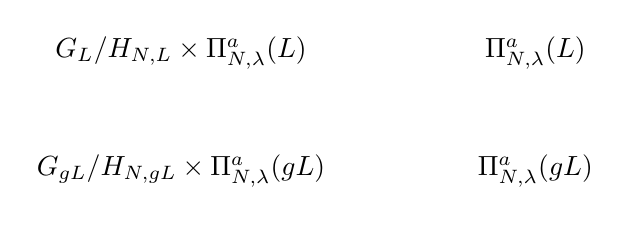
\begin{tikzpicture}[scale=1.5, baseline = -0.5ex]
\node (A) at (0,1) {$G_L/{H_{N,L}}\times\Pi_{N,\lambda}^a(L)$};
\node (B) at (3,1) {$\Pi_{N,\lambda}^a(L)$};
\node (C) at (0,0) {$G_{gL}/{H_{N,gL}}\times\Pi_{N,\lambda}^a(gL)$};
\node (D) at (3,0) {$\Pi_{N,\lambda}^a(gL)$};

\cdarrow (A) edge (B);
\cdarrow (A) edge (C);
\cdarrow (B) edge (D);
\cdarrow (C) edge (D);
\end{tikzpicture}
\end{equation*}

\subsection{Incidence in affine flag varieties}

Given $N,a,b,c\in\naturals$, $\lambda,\mu\in\compositions$, $L\in\flags$ and $i,j\in\integers$,
\begin{equation*}
\left\{(L',L'')\in\Pi_{N,\lambda}^a(L)\times\Pi_{N,\mu}^b(L): \dim\left(\frac{L_i'}{L_i'\cap L_j''}\right)\le c\right\}
\end{equation*}
is a closed set in $\Pi_{N,\lambda}^a(L)\times\Pi_{N,\mu}^b(L)$ since
\begin{equation*}
\dim\left(\frac{L_i'}{L_i'\cap L_j''}\right) = \dim\left(\frac{L_i'/{\epsilon^M L_0}}{L_i'/{\epsilon^M L_0}\cap L_j''/{\epsilon^M L_0}}\right).
\end{equation*}

\begin{lemma}\label{lemma:incidence-varieties-consequences}
Given $N,a,c\in\naturals$, $\lambda\in\compositions$, $L\in\flags$ and $i,j\in\integers$,
\begin{equation*}
\left\{L'\in\Pi_{N,\lambda}^a(L):\dim\left(\frac{L_i}{L_i\cap L_j'}\right)\le c\right\}
\end{equation*}
and
\begin{equation*}
\left\{L'\in\Pi_{N,\lambda}^a(L): \dim\left(\frac{L_j'}{L_i\cap L_j'}\right)\le c\right\}
\end{equation*}
are closed sets in $\Pi_{N,\lambda}^a(L)$.
\end{lemma}

\begin{proof}
This is a result of Lemma \ref{lemma:grassmannian-incidence-lemmas}, since
\begin{equation*}
\dim\left(\frac{L_i}{L_i\cap L_j'}\right) = \dim\left(\frac{L_i/{\epsilon^M L_0}}{L_i/{\epsilon^M L_0}\cap L_j'/{\epsilon^M L_0}}\right),
\end{equation*}
where $M\geq N$ is chosen so that $\epsilon^M L_0\subset L_i\subset\epsilon^{-M}L_0$ and $\epsilon^M L_0\subset L_j'\subset\epsilon^{-M}L_0$ for each $L'\in\Pi_{N,\lambda}^a(L)$.
\end{proof}


\section{Geometry of orbits}

Let $A\in\matrices$ and $L\in\flags_{\ro{A}}$ and write $\lambda=\co{A}$. Recall that
\begin{equation*}
\xprod[L]{A} = \{L'\in\flags_\lambda: (L,L')\in\orbit{A}\}.
\end{equation*}

\begin{lemma}\label{lemma:bounded-orbits}
There is $N\in\naturals$ such that $\xprod[L]{A}\subset\Pi_{N,\lambda}^a(L)$, where $a=d_{nN,0}{(A)}$.
\end{lemma}

\begin{proof}
There is $N\in\naturals$ so that $a_{i,j}=0$ whenever $|j-i|>nN$. If $(L,L')\in\orbit{A}$ then
\begin{equation*}
\dim\left(\frac{L_0'}{L_0'\cap\epsilon^{-N}L_0}\right) = \dim\left(\frac{L_0'}{L_0'\cap L_{nN}}\right) = \sum_{s>nN,t\le 0} a_{s,t} = 0,
\end{equation*}
so it follows $L_0'\subset\epsilon^{-N}L_0$. Similarly,
\begin{equation*}
\dim\left(\frac{\epsilon^N L_0}{\epsilon^N L_0\cap L_0'}\right) = \dim\left(\frac{L_{-nN}}{L_{-nN}\cap L_0'}\right) = \sum_{s\le -nN,t>0} a_{s,t} = 0,
\end{equation*}
which shows $\epsilon^N L_0\subset L_0'$. Moreover,
\begin{equation*}
\dim\left(\frac{\epsilon^{-N}L_0}{L_0'}\right) = \dim\left(\frac{\epsilon^{-N}L_0}{\epsilon^{-N}L_0\cap L_0'}\right) = \sum_{s\le nN,t>0}a_{s,t} = d_{nN,0}(A),
\end{equation*}
as a result of Lemma \ref{lemma:hook-codimension-formula}. 
\end{proof}

Assume $N\in\naturals$ is chosen so that $\xprod[L]{A}\subset\Pi_{N,\lambda}^a(L)$, where $a=d_{nN,0}{A}$, as in Lemma \ref{lemma:bounded-orbits}.

\begin{lemma}\label{lemma:orbits-are-quasiprojective}
$\xprod[L]{A}$ is a locally closed subset of $\Pi_{N,\lambda}^a(L)$. In particular, $\xprod[L]{A}$ is a quasiprojective variety.
\end{lemma}

\begin{proof}
If $L'\in\Pi_{N,\lambda}^a(L)$ then
\begin{equation*}
L_{-Nn}=\epsilon^N L_0\subset L_0'\subset L_1'\subset L_n'\subset \epsilon^{-1-N}L_0 = L_{(N+1)n}.
\end{equation*}
Therefore $\xprod[L]{A}$ is the subset of $\Pi_{N,\lambda}^a(L)$ defined by the conditions $\dim(L_i/{L_i\cap L_j'})=d_{i,j}{A}$ for $i:-Nn\le i<j$ and $\dim(L_j'/{L_i\cap L_j'})=\bar{d}_{i,j}{A}$ for $i:j<i\le(N+1)n$, for $j=1,\ldots,n$.

The set of $L'\in\Pi_{N,\lambda}^a(L)$ with $\dim(L_i/{L_i\cap L_j'})\le d_{i,j}{A}$ for $j=1,\ldots,n$ and $i:-Nn\le i<j$ and $\dim(L_j'/{L_i\cap L_j'})\le\bar{d}_{i,j}{A}$ for $j=1,\ldots,n$ and $i:j<i\le(N+1)n$ is a closed subset of $\Pi_{N,\lambda}^a(L)$, as a result of Lemma \ref{lemma:incidence-varieties-consequences}.

On the other hand, the set of $L'\in\Pi_{N,\lambda}^a(L)$ satisfying the conditions
\begin{equation*}
\dim(L_i/{L_i\cap L_j'})\geq d_{i,j}{A}
\end{equation*}
for $i<j$ and
\begin{equation*}
\dim(L_j'/{L_i\cap L_j'})\geq\bar{d}_{i,j}{A}
\end{equation*}
for $i>j$ is open in $\Pi_{N,\lambda}^a(L)$ since the complement is closed, as a result of Lemma \ref{lemma:incidence-varieties-consequences}.

Therefore $\xprod[L]{A}$ is the intersection of an open set and a closed set in $\Pi_{N,\lambda}^a(L)$, so $\xprod[L]{A}$ is locally closed. It follows that $\xprod[L]{A}$ is an open subset of the projective variety $\overline{\xprod[L]{A}}$, so is a quasiprojective variety as claimed.
\end{proof}

\begin{lemma}\label{lemma:orbits-are-irreducible}
$\xprod[L]{A}$ is irreducible.
\end{lemma}

\begin{proof}
For any $L'\in\xprod[L]{A}$, $\xprod[L]{A} = G_L/{H_{N,L}}\cdot L'$. Lemma \ref{lemma:connected-algebraic-group} shows that $G_L/{H_{N,L}}$ is a connected algebraic group which acts algebraically on $\Pi_{N,\lambda}^a(L)$. The image of $G_L/{H_{N,L}}$ under the morphism $g\mapsto gL'$ equals $\xprod[L]{A}$, which shows $\xprod[L]{A}$ is irreducible since $G_L/{H_{N,L}}$ is irreducible.
\end{proof}

Consequently, $\overline{\xprod[L]{A}}$ is an irreducible projective variety and the action of $G_L/{H_{N,L}}$ on $\Pi_{N,\lambda}^a(L)$ restricts to an algebraic group action on $\overline{\xprod[L]{A}}$ for which there are finitely many orbits. In particular, $\overline{\xprod[L]{A}}\setminus\xprod[L]{A}$ is a union of finitely many orbits which are so-called degenerations of the orbit $\xprod[L]{A}$.


\section{Geometry of orbit products}

Let $A,B\in\matrices$ with $\co{A}=\ro{B}$ and write $\lambda=\co{A}$ and $\mu=\co{B}$. Fix $L\in\flags_{\ro{A}}$. Recall
\begin{equation*}
\yprod[L]{A,B}=\{(L',L'')\in\flags_{\lambda}\times\flags_{\mu}: L'\in\xprod[L]{A}, L''\in\xprod[L']{B}\}
\end{equation*}
and
\begin{equation*}
\xprod[L]{A,B}=\{L''\in\flags_{\mu}: \exists L' \text{ with } (L',L'')\in\yprod[L]{A,B}\}.
\end{equation*}

\begin{lemma}\label{lemma:embedding-orbit-products}
There is $N\in\naturals$ such that
\begin{equation*}
\yprod[L]{A,B}\subset\Pi_{N,\lambda}^a(L)\times\Pi_{2N,\mu}^{a+b}(L),
\end{equation*}
where $a=d_{nN,0}{(A)}$ and $b=d_{nN,0}{(B)}$.
\end{lemma}

\begin{proof}
There is $N\in\naturals$ such that $\epsilon^N{L_0}\subset L_0'\subset\epsilon^{-N}L_0$ and $\epsilon^NL_0'\subset L_0''\subset\epsilon^{-N}L_0'$ for each $(L',L'')\in\yprod[L]{A,B}$, using Lemma \ref{lemma:bounded-orbits}. Set $a=d_{nN,0}{(A)}$ and $b=d_{nN,0}{(B)}$.

Then for any $(L',L'')\in\yprod[L]{A,B}$,
\begin{equation*}
\epsilon^{2N}L_0\subset\epsilon^NL_0'\subset L_0''\subset\epsilon^{-N}L_0'\subset\epsilon^{-2N}L_0
\end{equation*}
and
\begin{align*}
\dim\left(\frac{\epsilon^{-2N}L_0}{L_0''}\right)
&=\dim\left(\frac{\epsilon^{-N}L_0'}{L_0''}\right) + \dim\left(\frac{\epsilon^{-2N}L_0}{\epsilon^{-N}L_0'}\right)\\
&=\dim\left(\frac{\epsilon^{-N}L_0'}{L_0''}\right) + \dim\left(\frac{\epsilon^{-N}L_0}{L_0'}\right)\\
&= a+b,
\end{align*}
as a result of Lemma \ref{lemma:hook-codimension-formula}, so $(L',L'')\in\Pi_{N,\lambda}^a(L)\times\Pi_{2N,\mu}^{a+b}(L)$ as required.
\end{proof}

Now assume $N\in\naturals$ is chosen so that $\yprod[L]{A,B}\subset\Pi_{N,\lambda}^a(L)\times\Pi_{2N,\mu}^{a+b}(L)$, where $a=d_{nN,0}{(A)}$ and $b=d_{nN,0}{(B)}$, using Lemma \ref{lemma:embedding-orbit-products}.

\begin{lemma}\label{lemma:y-prod-is-quasiprojective}
$\yprod[L]{A,B}$ is a locally closed subset of $\Pi_{N,\lambda}^a(L)\times\Pi_{2N,\mu}^{a+b}(L)$. In particular, $\yprod[L]{A,B}$ is a quasiprojective variety.
\end{lemma}

\begin{proof}
$\yprod[L]{A,B}$ is the subset of $\Pi_{N,\lambda}^a(L)\times\Pi_{2N,\mu}^{a+b}(L)$ consisting of those $(L',L'')$ satisfying the following conditions: $\dim(L_i/{L_i\cap L_j'}) = d_{i,j}{(A)}$ for $i<j$, $\dim(L_j'/{L_i\cap L_j'})=\bar{d}_{i,j}{(A)}$ for $i>j$, $\dim(L_i'/{L_i'\cap L_j''})=d_{i,j}{(B)}$ for $i<j$ and $\dim(L_j''/{L_i'\cap L_j''})=\bar{d}_{i,j}{(B)}$. Only finitely many conditions are required to define $\yprod[L]{A,B}$ since there are only finitely many nonzero entries in $A$ and $B$ modulo the $(n,n)$-periodicity.

The conditions
\begin{align*}
\dim(L_i/{L_i\cap L_j'}) &\le d_{i,j}{(A)}\\
\dim(L_i'/{L_i'\cap L_j''}) &\le d_{i,j}{(B)}\\
\dim(L_j'/{L_i\cap L_j'}) &\le\bar{d}_{i,j}{(A)}\\
\dim(L_j''/{L_i'\cap L_j''}) &\le\bar{d}_{i,j}{(B)}
\end{align*}
define closed subsets of $\Pi_{N,\lambda}^a(L)\times\Pi_{2N,\mu}^{a+b}(L)$ for each $i,j\in\integers$, as a result of Lemma \ref{lemma:incidence-varieties-consequences}.

On the other hand, the conditions
\begin{align*}
\dim(L_i/{L_i\cap L_j'}) &\geq d_{i,j}{(A)}\\
\dim(L_i'/{L_i'\cap L_j''}) &\geq d_{i,j}{(B)}\\
\dim(L_j'/{L_i\cap L_j'}) &\geq \bar{d}_{i,j}{(A)}\\
\dim(L_j''/{L_i'\cap L_j''}) &\geq \bar{d}_{i,j}{(B)}
\end{align*}
define open subsets of $\Pi_{N,\lambda}^a(L)\times\Pi_{2N,\mu}^{a+b}(L)$ for each $i,j\in\integers$, using Lemma \ref{lemma:incidence-varieties-consequences}.

Therefore $\yprod[L]{A,B}$ is the intersection of finitely many open sets and finitely many closed sets in $\Pi_{N,\lambda}^a(L)\times\Pi_{2N,\mu}^{a+b}(L)$, so $\yprod[L]{A,B}$ is locally closed. In particular, $\yprod[L]{A,B}$ is a quasiprojective variety.
\end{proof}

\begin{lemma}\label{lemma:yprod-as-a-saturation}
For any $L'\in\xprod[L]{A}$,
\begin{equation*}
\yprod[L]{A,B} = G_L\cdot(\{L'\}\times\xprod[L']{B}).
\end{equation*}
\end{lemma}

\begin{proof}
Let $L'\in\xprod[L]{A}$, then $\{L'\}\times\xprod[L']{B}$ is contained in $\yprod[L]{A,B}$ and $G_L$ acts on $\yprod[L]{A,B}$, so $G_L\cdot(\{L'\}\times\xprod[L']{B})$ is contained in $\yprod[L]{A,B}$. If $(N',N'')\in\yprod[L]{A,B}$, then $N'=\sigma L'$ for some $\sigma\in G_L$, since $N'\in\xprod[L]{A}$. Then $(N',N'')=\sigma (L',\sigma^{-1}N'')$ and $\sigma^{-1}N''\in\xprod[\sigma^{-1}N']{B}=\xprod[L']{B}$, so $(N',N'')\in\sigma\cdot(\{L'\}\times\xprod[L']{B})$. Therefore $\yprod[L]{A,B}=G_L\cdot(\{L'\}\times\xprod[L']{B})$ as claimed.
\end{proof}

\begin{proposition}\label{prop:irreducible-y-prod}
$\yprod[L]{A,B}$ is irreducible.
\end{proposition}

\begin{proof}
Let $L'\in\xprod[L]{A}$. $G_L/{H_{2N,L}}$ is a connected algebraic group acting algebraically on $\Pi_{N,\lambda}^a(L)\times\Pi_{2N,\mu}^{a+b}(L)$ by Lemma \ref{lemma:connected-algebraic-group}. $\xprod[L']{B}$ is an irreducible locally closed subset of $\Pi_{2N,\mu}^{a+b}(L)$, so $\{L'\}\times\xprod[L']{B}$ is an irreducible locally closed set in $\Pi_{N,\lambda}^a(L)\times\Pi_{2N,\mu}^{a+b}(L)$. $\yprod[L]{A,B}=G_L\cdot (\{L'\}\times\xprod[L']{B}) = G_L/{H_{2N,L}}\cdot (\{L'\}\times\xprod[L']{B})$, by Lemma \ref{lemma:yprod-as-a-saturation}, so it follows that $\yprod[L]{A,B}$ is irreducible.
\end{proof}

Let $p_2$ be the projection onto the second factor $\Pi_{N,\lambda}^a(L)\times\Pi_{2N,\mu}^{a+b}(L)\to\Pi_{2N,\mu}^{a+b}(L)$. $p_2$ is a closed morphism since $\Pi_{N,\lambda}^a(L)$ is a projective variety and therefore complete, by Lemma \ref{lemma:projective-varieties-of-cyclic-flags}. Therefore $p_2(\overline{\yprod[L]{A,B}})=\overline{\xprod[L]{A,B}}$, since $p_2(\yprod[L]{A,B})=\xprod[L]{A,B}$.

\begin{lemma}\label{lemma:irreducible-x-prod}
$\xprod[L]{A,B}$ is irreducible and constructible.
\end{lemma}

\begin{proof}
Proposition \ref{prop:irreducible-y-prod} shows that $\yprod[L]{A,B}$ is irreducible and locally closed, so it follows $\xprod[L]{A,B}$ is irreducible and constructible, since $\xprod[L]{A,B}=p_2(\yprod[L]{A,B})$.
\end{proof}

\begin{proposition}\label{prop:open-orbit-x-prod}
There is a unique open $G_L$-orbit in $\xprod[L]{A,B}$.
\end{proposition}

\begin{proof}
$\xprod[L]{A,B}$ consists of finitely many $G_L$-orbits and is an irreducible topological space, by Lemma \ref{lemma:irreducible-x-prod}. Consequently, $\xprod[L]{C}$ is dense in $\xprod[L]{A,B}$ for some $C\in\matrices^{A,B}$. Lemma \ref{lemma:orbits-are-quasiprojective} shows that $\xprod[L]{C}$ is locally closed in $\xprod[L]{A,B}$, so $\xprod[L]{C}$ is open in $\overline{\xprod[L]{C}}=\xprod[L]{A,B}$. Irreducibility of $\xprod[L]{A,B}$ shows that there is a unique open $G_L$-orbit, since two nonempty open sets in $\xprod[L]{A,B}$ intersect nontrivially, thus any two open $G_L$ orbits in $\xprod[L]{A,B}$ coincide.
\end{proof}

Let $A\ast B\in\matrices$ denote the matrix corresponding to the dense open $G_L$-orbit in $\xprod[L]{A,B}$, so $\overline{\xprod[L]{A\ast B}}=\overline{\xprod[L]{A,B}}$.

\section{Degenerations of orbits and the combinatorial partial order}

\begin{proposition}\label{proposition:compare-partial-orders}
Let $A,B\in\matrices$ with $\ro{A}=\ro{B}$ and $\co{A}=\co{B}$. If $\xprod[L]{B}\subset\overline{\xprod[L]{A}}$ for some $L\in\flags_{\ro{A}}$ then $B\le A$ with respect to the hook order.
\end{proposition}

\begin{proof}
Let $\lambda=\co{A}$, $\mu=\ro{A}$ and fix $L\in\flags_\mu$. Assume $N\in\naturals$ is chosen so that $\xprod[L]{A}\subset\Pi_{N,\lambda}^a(L)$ and $\xprod[L]{B}\subset\Pi_{N,\lambda}^b(L)$, where $a=d_{nN,0}{(A)}$ and $b=d_{nN,0}{(B)}$. Then $\xprod[L]{A}$ is an open subset of the projective variety consisting of those $L'\in\Pi_{N,\lambda}^a(L)$ such that
\begin{equation*}
\dim\left(\frac{L_i}{L_i\cap L_j'}\right)\le d_{i,j}{(A)}
\end{equation*}
and
\begin{equation*}
\dim\left(\frac{L_j'}{L_i\cap L_j'}\right)\le\bar{d}_{i,j}{(A)},
\end{equation*}
for all $i,j\in\integers$.

Assume $\xprod[L]{B}\subset \overline{\xprod[L]{A}}$, then
\begin{equation*}
d_{i,j}{(B)} = \dim\left(\frac{L_i}{L_i\cap L_j'}\right) \le d_{i,j}{(A)}
\end{equation*}
and
\begin{equation*}
\bar{d}_{i,j}{(B)} = \dim\left(\frac{L_j'}{L_i\cap L_j'}\right) \le \bar{d}_{i,j}{(A)},
\end{equation*}
for each $i,j\in\integers$, for any $L'\in\xprod[L]{B}$. So $B\le A$ if $\xprod[L]{B}\le\overline{\xprod[L]{A}}$.
\end{proof}

\begin{remark}
In practice it seems that the converse of Proposition \ref{proposition:compare-partial-orders} is true, so that the closure order and the hook order are the same, although I have not been able to find a proof.
\end{remark}

\begin{corollary}
\begin{equation*}
A\ast B = \max\{C\in\matrices: g_{A,B,C}\neq 0\}
\end{equation*}
\end{corollary}


\section{Associativity of the generic product}

Let $A,B,C\in\matrices$ with $\co{A}=\ro{B}$ and $\co{B}=\ro{C}$ and fix $L\in\flags_{\ro{A}}$. Write $\lambda=\co{A}$, $\mu=\co{B}$ and $\nu=\co{C}$. Define
\begin{equation*}
\yprod[L]{A,B,C} = \left\{(L',L'',L''')\in\flags^3: L'\in\xprod[L]{A}, L''\in\xprod[L']{B}, L'''\in\xprod[L'']{C}\right\}
\end{equation*}
and
\begin{equation*}
\xprod[L]{A,B,C} = \left\{L'''\in\flags: \exists (L',L'')\in\flags^2 \text{ with } (L',L'',L''')\in\yprod[L]{A,B,C}\right\}.
\end{equation*}

\begin{lemma}\label{lemma:embedding-y-triple}
There is $N\in\naturals$ such that $\yprod[L]{A,B,C}$ is contained in
\begin{equation*}
\Pi_{N,\lambda}^a(L)\times\Pi_{2N,\mu}^{a+b}(L)\times\Pi_{3N,\nu}^{a+b+c}(L),
\end{equation*}
where $a=d_{nN,0}{(A)}$, $b=d_{nN,0}{(B)}$ and $c=d_{nN,0}{(C)}$.
\end{lemma}

\begin{proof}
Lemma \ref{lemma:bounded-orbits} shows that there is $N\in\naturals$ such that $\epsilon^N L_0\subset L_0'\subset\epsilon^{-N}L_0$, $\epsilon^N L_0'\subset L_0''\subset\epsilon^{-N}L_0'$ and $\epsilon^N L_0''\subset L_0'''\subset\epsilon^{-N}L_0''$ for each $(L',L'',L''')\in\yprod[L]{A,B,C}$. Using the proof of Lemma \ref{lemma:embedding-orbit-products}, it follows $L''\in\Pi_{2N,\mu}^{a+b}(L)$ and $L'''\in\Pi_{2N,\nu}^{b+c}(L')\subset\Pi_{3N,\nu}^{a+b+c}(L)$.
\end{proof}

Assume $N\in\naturals$ is chosen so that $\yprod[L]{A,B,C}\subset\Pi_{N,\lambda}^a(L)\times\Pi_{2N,\mu}^{a+b}(L)\times\Pi_{3N,\nu}^{a+b+c}(L)$, where $a=d_{nN,0}{(A)}$, $b=d_{nN,0}{(B)}$ and $c=d_{nN,0}{(C)}$, as in Lemma \ref{lemma:embedding-y-triple}.

\begin{lemma}\label{lemma:y-triple-is-quasiprojective}
$\yprod[L]{A,B,C}$ is a locally closed subset of $\Pi_{N,\lambda}^a(L)\times\Pi_{2N,\mu}^{a+b}(L)\times\Pi_{3N,\nu}^{a+b+c}(L)$. In particular, $\yprod[L]{A,B,C}$ is a quasiprojective variety.
\end{lemma}

\begin{proof}
Write $\Pi=\Pi_{N,\lambda}^a(L)\times\Pi_{2N,\mu}^{a+b}(L)\times\Pi_{3N,\nu}(L)$. Then $\yprod[L]{A,B,C}$ consists of those $(L',L'',L''')\in\Pi$ satisfying the following conditions:
\begin{align}
\dim\left(\frac{L_i}{L_i\cap L_j'}\right) &= d_{i,j}{(A)},\\
\dim\left(\frac{L_i'}{L_i'\cap L_j''}\right) &= d_{i,j}{(B)},\\
\dim\left(\frac{L_i''}{L_i''\cap L_j'''}\right) &= d_{i,j}{(C)},
\end{align}
for $(i,j)\in \{1,\ldots,n\}\times\integers$ with $i<j<(N+1)n$, and
\begin{align}
\dim\left(\frac{L_j'}{L_i\cap L_j'}\right) &= \bar{d}_{i,j}{(A)},\\
\dim\left(\frac{L_j''}{L_i'\cap L_j''}\right) &= \bar{d}_{i,j}{(B)},\\
\dim\left(\frac{L_j'''}{L_i''\cap L_j'''}\right) &= \bar{d}_{i,j}{(C)},
\end{align}
for $(i,j)\in \{1,\ldots,n\}\times\integers$ with $-Nn<j<i$.

For $i<j$, the conditions
\begin{align*}
\dim\left(\frac{L_i}{L_i\cap L_j'}\right) &\le d_{i,j}{(A)}\\
\dim\left(\frac{L_i'}{L_i'\cap L_j''}\right) &\le d_{i,j}{(B)}\\
\dim\left(\frac{L_i''}{L_i''\cap L_j'''}\right) &\le d_{i,j}{(C)}
\end{align*}
define closed subsets of $\Pi$.

For $i>j$, the conditions
\begin{align*}
\dim\left(\frac{L_j'}{L_i\cap L_j'}\right) &\le \bar{d}_{i,j}{(A)}\\
\dim\left(\frac{L_j''}{L_i'\cap L_j''}\right) &\le \bar{d}_{i,j}{(B)}\\
\dim\left(\frac{L_j'''}{L_i''\cap L_j'''}\right) &\le \bar{d}_{i,j}{(C)}
\end{align*}
also define closed subsets of $\Pi$.

On the other hand, the conditions
\begin{align*}
\dim\left(\frac{L_i}{L_i\cap L_j'}\right) &\geq d_{i,j}{(A)}\\
\dim\left(\frac{L_i'}{L_i'\cap L_j''}\right) &\geq d_{i,j}{(B)}\\
\dim\left(\frac{L_i''}{L_i''\cap L_j'''}\right) &\geq d_{i,j}{(C)}
\end{align*}
define open subsets of $\Pi$ for $i<j$. Similarly, the conditions
\begin{align*}
\dim\left(\frac{L_j'}{L_i\cap L_j'}\right) &\geq \bar{d}_{i,j}{(A)}\\
\dim\left(\frac{L_j''}{L_i'\cap L_j''}\right) &\geq \bar{d}_{i,j}{(B)}\\
\dim\left(\frac{L_j'''}{L_i''\cap L_j'''}\right) &\geq \bar{d}_{i,j}{(C)}
\end{align*}
define open subsets of $\Pi$ for $i>j$.

Therefore $\yprod[L]{A,B,C}$ is the intersection of finitely many closed sets in $\Pi$ with finitely many open subsets of $\Pi$, so $\yprod[L]{A,B,C}$ is locally closed. In particular, $\yprod[L]{A,B,C}$ is a quasiprojective variety.
\end{proof}

\begin{lemma}\label{lemma:y-triple-stabilisers}
For any $(L',L'',L''')\in\yprod[L]{A,B,C}$,
\begin{equation*}
\yprod[L]{A,B,C} = \left\{ \alpha\cdot (L',\beta L'',\beta\gamma L'''): \alpha\in G_L, \beta\in G_{L'}, \gamma\in G_{L''}\right\}.
\end{equation*}
In particular,
\begin{equation*}
\yprod[L]{A,B,C} = G_L\cdot\left(\{L'\}\times\yprod[L']{B,C}\right)
\end{equation*}
for each $L'\in\xprod[L]{A}$.
\end{lemma}

\begin{proof}
Let $(L',L'',L''')\in\yprod[L]{A,B,C}$. If $\alpha\in G_{L}$, $\beta\in G_{L'}$ and $\gamma\in G_{L''}$ then
\begin{equation*}
(\alpha L',\alpha\beta L'', \alpha\beta\gamma L''')\in\yprod[L]{A,B,C}
\end{equation*}
since
\begin{align*}
(L,\alpha L') &= \alpha (L,L')\in\orbit{A}\\
(\alpha L', \alpha\beta L'') &= \alpha\beta (L',L'')\in\orbit{B}\\
(\alpha\beta L'',\alpha\beta\gamma L''') &= \alpha\beta\gamma (L'',L''')\in\orbit{C}
\end{align*}

For each $(N',N'',N''')\yprod[L]{A,B,C}$ there exist $\sigma_1,\sigma_2,\sigma_3\in G$ with
\begin{align*}
(L,N') &= \sigma_1(L,L')\\
(N',N'') &= \sigma_2(L',L'')\\
(N'',N''') &= \sigma_3(L'',L''').
\end{align*}

Let $\alpha = \sigma_1$, $\beta = \sigma_1^{-1}\sigma_2$ and $\gamma = \sigma_2^{-1}\sigma_3$, so $\sigma_2=\alpha\beta$ and $\sigma_3=\alpha\beta\gamma$. It follows that
\begin{equation*}
(N',N'',N''') = (\alpha L',\alpha\beta L'', \alpha\beta\gamma L'''),
\end{equation*}
which proves the first claim. The second claim follows from the first since $(L'',L''')\in\yprod[L']{B,C}$ and therefore
\begin{equation*}
\yprod[L']{B,C} = \{(\beta L'',\beta\gamma L'''):\beta\in G_{L'}, \gamma\in G_{L''}\},
\end{equation*}
as required.
\end{proof}

\begin{proposition}\label{proposition:irreducible-y-triple}
$\yprod[L]{A,B,C}$ is irreducible.
\end{proposition}

\begin{proof}
Write
\begin{equation*}
\Pi=\Pi_{N,\lambda}^{a}(L)\times\Pi_{2N,\mu}^{a+b}(L)\times\Pi_{3N,\nu}^{a+b+c}(L).
\end{equation*}

Lemma $\ref{lemma:projective-varieties-of-cyclic-flags}$ shows that $\Pi$ is a projective algebraic variety and Lemma \ref{lemma:connected-algebraic-group} shows that $G_L/{H_{3N,L}}$ is a connected algebraic group acting algebraically on $\Pi$ by the diagonal action.

Let $L'\in\xprod[L]{A}$. As a result of Lemma \ref{lemma:y-triple-stabilisers} 
\begin{align*}
\yprod[L]{A,B,C}
&= G_L\cdot (\{L'\}\times\yprod[L']{B,C})\\
&= G_L/{H_{3N,L}}\cdot (\{L'\}\times\yprod[L']{B,C}).
\end{align*}

Proposition \ref{prop:irreducible-y-prod} shows that $\yprod[L']{B,C}$ is irreducible, so $\{L'\}\times\yprod[L']{B,C}$ is irreducible. The image of $\{L'\}\times\yprod[L']{B,C}$ under the action of $G_L/{H_{3N,L}}$ is irreducible, since $G_L/{H_{3N,L}}$ is connected and therefore irreducible. Therefore $\yprod[L]{A,B,C}$ is irreducible.
\end{proof}

Let $p_3$ be the projection of $\Pi_{N,\lambda}^a(L)\times\Pi_{2N,\mu}^{a+b}(L)\times\Pi_{3N,\nu}^{a+b+c}(L)$ onto the third factor. By the completeness property of projective varieties, $p_3$ is a closed morphism. The image of $\yprod[L]{A,B,C}$ under $p_3$ is $\xprod[L]{A,B,C}$, so $p_3(\overline{\yprod[L]{A,B,C}}) = \overline{\xprod[L]{A,B,C}}$.

\begin{lemma}\label{lemma:irreducible-x-triple}
$\xprod[L]{A,B,C}$ is irreducible and constructible.
\end{lemma}

\begin{proof}
Lemma \ref{lemma:y-triple-is-quasiprojective} and Proposition \ref{proposition:irreducible-y-triple} show that $\yprod[L]{A,B,C}$ is locally closed and irreducible. It follows $\xprod[L]{A,B}$ is irreducible and constructible, since $\xprod[L]{A,B,C}$ is the image of $\yprod[L]{A,B,C}$ under the morphism $p_3$.
\end{proof}

\begin{lemma}\label{lemma:generic-triple-product}
There is a unique open and dense $G_L$-orbit in $\xprod[L]{A,B,C}$.
\end{lemma}

\begin{proof}
There are only finitely many $G_L$-orbits in $\xprod[L]{A,B,C}$. In particular,
\begin{equation*}
\xprod[L]{A,B,C}=\bigcup_{D\in\matrices^{A,B}}\xprod[L]{D,C}=\bigcup_{D\in\matrices^{A,B}}\bigcup_{D'\in\matrices^{D,C}}\xprod[L]{D'}
\end{equation*}
and
\begin{equation*}
\overline{\xprod[L]{A,B,C}} = \bigcup_{D\in\matrices^{A,B}}\bigcup_{D'\in\matrices^{D,C}}\overline{\xprod[L]{D'}}.
\end{equation*}
There is $D\in\matrices$ such that $\overline{\xprod[L]{D}}=\overline{\xprod[L]{A,B,C}}$, since $\xprod[L]{A,B,C}$ is irreducible, by Lemma \ref{lemma:irreducible-x-triple}. By Lemma \ref{lemma:orbits-are-quasiprojective}, $\xprod[L]{D}$ is open in $\overline{\xprod[L]{D}}=\overline{\xprod[L]{A,B,C}}$, so $\xprod[L]{D}$ is open in $\xprod[L]{A,B,C}$.

If $\xprod[L]{D}$ and $\xprod[L]{D'}$ are open in $\xprod[L]{A,B,C}$, then $\xprod[L]{D}$ and $\xprod[L]{D'}$ have nonempty intersection since $\xprod[L]{A,B,C}$ is irreducible, then $\xprod[L]{D}=\xprod[L]{D'}$.
\end{proof}

\begin{lemma}\label{lemma:yprod-generic-A-B}
$p_3^{-1}(\xprod[L]{A\ast B,C})$ is open in $\overline{\yprod[L]{A,B,C}}$.
\end{lemma}

\begin{proof}
Projection onto the second component is a closed morphism of varieties $p_2\colon\overline{\yprod[L]{A,B,C}}\to\overline{\xprod[L]{A,B}}$ with $p_2(\yprod[L]{A,B,C})=\xprod[L]{A,B}$. It follows that $p_3^{-1}(\xprod[L]{A\ast B,C})$ is open in $\overline{\yprod[L]{A,B,C}}$ since $p_3^{-1}(\xprod[L]{A\ast B,C})=p_2^{-1}(\xprod[L]{A\ast B})$ and $\xprod[L]{A\ast B}$ is open in $\overline{\xprod[L]{A,B}}$.
\end{proof}

\begin{lemma}\label{lemma:yprod-generic-B-C}
$p_3^{-1}(\xprod[L]{A,B\ast C})$ is an open subset of $\overline{\yprod[L]{A,B,C}}$.
\end{lemma}

\begin{proof}
$p_3^{-1}(\xprod[L]{A,B\ast C})$ consists of those $(L',L'',L''')\in\overline{\yprod[L]{A,B,C}}$ such that
\begin{equation*}
\dim\left(\frac{L_i'}{L_i'\cap L_j'''}\right)\geq d_{i,j}(B\ast C)
\end{equation*}
for $i<j$ and
\begin{equation*}
\dim\left(\frac{L_j'''}{L_i'\cap L_j'''}\right)\geq\bar{d}_{i,j}(B\ast C)
\end{equation*}
for $i,j\in\integers$ with $i>j$. Each of these conditions defines an open subset of $\overline{\yprod[L]{A,B,C}}$and $p_3^{-1}(\xprod[L]{A,B\ast C})$ is determined by only finitely many of the conditions, so is the intersection of finitely many open sets in $\overline{\yprod[L]{A,B,C}}$, so $p_3^{-1}(\xprod[L]{A,B\ast C})$ is open in $\yprod[L]{A,B,C}$.
\end{proof}

\begin{theorem}\label{theorem:associativity}
\begin{equation*}
\xprod[L]{A\ast (B\ast C)} = \xprod[L]{(A\ast B)\ast C}.
\end{equation*}
\end{theorem}

\begin{proof}
The unique open $G_L$-orbit in $\xprod[L]{A\ast B, C}$ is $\xprod[L]{(A\ast B)\ast C}$, so $p_3^{-1}(\xprod[L]{(A\ast B)\ast C})$ is open in $p_3^{-1}(\xprod[L]{A\ast B,C})$ and Lemma \ref{lemma:yprod-generic-A-B} shows that $p_3^{-1}(\xprod[L]{A\ast B,C})$ is open in $\overline{\yprod[L]{A,B,C}}$, so $p_3^{-1}(\xprod[L]{(A\ast B)\ast C})$ is open in $\overline{\yprod[L]{A,B,C}}$.

Similarly, $\xprod[L]{A\ast (B\ast C)}$ is open in $\xprod[L]{A,B\ast C}$, so $p_3^{-1}(\xprod[L]{A\ast (B\ast C)})$ is open in $p_3^{-1}(\xprod[L]{A,B\ast C})$ and Lemma \ref{lemma:yprod-generic-B-C} shows that $p_3^{-1}(\xprod[L]{A,B\ast C})$ is open in $\overline{\yprod[L]{A,B,C}}$, so it follows that $p_3^{-1}(\xprod[L]{A\ast (B\ast C)})$ is open in $\overline{\yprod[L]{A,B,C}}$.

Therefore the intersection of $p_3^{-1}(\xprod[L]{A\ast (B\ast C)})$ with $p_3^{-1}(\xprod[L]{(A\ast B)\ast C})$ is nonempty since $\yprod[L]{A,B,C}$ is irreducible, by Proposition \ref{proposition:irreducible-y-triple}. It follows that the $G_L$-orbits $\xprod[L]{A\ast (B\ast C)}$ and $\xprod[L]{(A\ast B)\ast C}$ have nonempty intersection and therefore are the same orbit.
\end{proof}


\section{The generic affine algebra and a catagorical perspective}

The generic affine algebra of rank $r$ and period $n$, denoted by $\generic$, is a free $\integers$-module with basis $\{e_A:A\in\matrices\}$ and $\integers$-bilinear multiplication given by
\begin{equation*}
e_A\ast e_B = e_{A\ast B}
\end{equation*}
for $A,B\in\matrices$ with $\co{A}=\ro{B}$, and
\begin{equation*}
e_A\ast e_B = 0
\end{equation*}
for $A,B\in\matrices$ with $\co{A}\neq\ro{B}$.

\begin{theorem}\label{theorem:generic-algebra-associative}
The generic algebra $\generic$ is an associative $\integers$-algebra with $1$, with
\begin{equation*}
1=\sum_{\lambda\in\compositions} 1_\lambda
\end{equation*}
where
\begin{equation*}
1_\lambda = e_{\diag{\lambda}},
\end{equation*}
for each $\lambda\in\compositions$.
\end{theorem}

\begin{proof}
Let $A,B,C\in\matrices$. If $\co{A}\neq\ro{B}$ or $\co{B}\neq\ro{C}$, then
\begin{equation*}
(e_A\ast e_B)\ast e_C = 0 = e_A\ast (e_B\ast e_C),
\end{equation*}
so we may now suppose $\co{A}=\ro{B}$ and $\co{B}=\ro{C}$.

As a result of Theorem \ref{theorem:associativity},
\begin{align*}
(e_A\ast e_B)\ast e_C &= e_{(A\ast B)\ast C}\\
&= e_{A\ast (B\ast C)}\\
&= e_A\ast (e_B\ast e_C),
\end{align*}
so it follows $\generic$ is an associative $\integers$-algebra.

The expression for the multiplicative identity follows from Lemma \ref{lemma:product-with-diagonal-orbits}, since
\begin{equation*}
e_A\ast \left(\sum_{\lambda\in\compositions} 1_\lambda\right) = e_A\ast 1_{\co{A}} = e_A
\end{equation*}
and
\begin{equation*}
\left(\sum_{\lambda\in\compositions} 1_\lambda\right)\ast e_A = 1_{\ro{A}}\ast e_A = e_A,
\end{equation*} 
for each $A\in\matrices$.
\end{proof}

\begin{proposition}\label{prop:generic-category}
The following constitutes a small category: the set of objects is $\compositions$ and the set of morphisms is $\matrices$. Given compositions $\lambda,\mu\in\compositions$, the morphisms with source $\mu$ and target $\lambda$ are those matrices $A\in\matrices$ with $\co{A}=\mu$ and $\ro{A}=\lambda$. Given $\lambda,\mu,\nu\in\compositions$ and $A,B\in\matrices$ with $\co{B}=\nu$, $\ro{B}=\mu=\co{A}$ and $\ro{A}=\lambda$, their composition is $A\ast B$, with source $\co{A\ast B}=\co{B}=\nu$ and target $\ro{A\ast B}=\ro{A}=\lambda$.
\end{proposition}

\begin{proof}
Theorem \ref{theorem:associativity} shows that the generic product $\ast$ is associative. For each object $\lambda\in\compositions$, the identity morphism $\lambda\to\lambda$ is the diagonal matrix $\diag{\lambda}$.
\end{proof}

Then the generic affine algebra $\generic$ may be realised as the $\integers$-algebra of this category. Observe that there are only finitely many objects in this category and distinct objects are non-isomorphic, so the isomorphism classes in this category are in one to one correspondence with $\compositions$. The $\integers$-algebra of this category is the free $\integers$-module on $\matrices$ with $\integers$-bilinear multiplication given by the generic product $\ast$.



\chapter{Towards a realisation of affine zero Schur algebras}\label{chapter:affine-0-schur}

The purpose of this chapter is to study the link between the generic affine algebra $\generic$ and the affine $0$-Schur algebra $\zeroschur$.

The main result is the construction of an isomorphism of $\integers$-algebras from $\generic$ to $\zeroschur$ such that $E_i\mapsto E_i$, $F_i\mapsto F_i$ and $1_\lambda\mapsto 1_\lambda$, in the case that $n,r\geq 1$ with $r<n$.

\section{Preliminary results on the generic affine algebra}

Recall from Chapter \ref{chapter:generic-affine-algebra} that the generic affine algebra $\generic$ is an associative $\integers$-algebra which is a free $\integers$-module on $\{e_A:A\in\matrices\}$ with multiplication defined by
\begin{equation*}
e_A\ast e_B = \begin{cases}
e_{A\ast B} &: \co{A}=\ro{B}\\
0 &: \co{A}\neq\ro{B}
\end{cases}
\end{equation*}
for $A,B\in\matrices$.

For $i\in\modn$ and $\lambda\in\compositions$ such that $\lambda_{i+1}>0$, define
\begin{equation*}
E_{i,\lambda} = e_{\diag{\lambda} + \elem{i}{i+1} - \elem{i+1}{i+1}}
\end{equation*}
and let
\begin{equation*}
E_i = \sum_{\lambda\in\compositions:\lambda_{i+1}>0} E_{i,\lambda}
\end{equation*}
for each $i\in\modn$

For $i\in\modn$ and $\lambda\in\compositions$ such that $\lambda_i>0$, define
\begin{equation*}
F_{i,\lambda} = e_{\diag{\lambda} + \elem{i+1}{i} - \elem{i}{i}}
\end{equation*}
and let
\begin{equation*}
F_i = \sum_{\lambda\in\compositions:\lambda_i>0} F_{i,\lambda}
\end{equation*}
for each $i\in\modn$.

\begin{lemma}\label{lemma:fundamental-multiplication-rule-generic}
Let $i\in\modn$ and $A\in\matrices$ and write $\mu=\ro{A}$.

If $\mu_{i+1}=0$ then $E_i\ast e_A=0$. If $\mu_{i+1}>0$, then
\begin{equation*}
E_i\ast e_A = e_{A+\elem{i}{p}-\elem{i+1}{p}},
\end{equation*}
where
\begin{equation*}
p=\max\{j\in\integers:a_{i+1,j}>0\}.
\end{equation*}

If $\mu_i=0$ then $F_i\ast e_A=0$. If $\mu_i>0$ then
\begin{equation*}
F_i\ast e_A = e_{A+\elem{i+1}{p}-\elem{i}{p}},
\end{equation*}
where
\begin{equation*}
p=\min\{j\in\integers: a_{i,j}>0\}.
\end{equation*}
\end{lemma}

\begin{proof}
The corresponding product in the affine $q$-Schur algebra $\qschur$ is
\begin{equation*}
E_i\cdot e_A = \sum_{j\in\integers:a_{i+1,j}>0} q^{\sum_{t>j} a_{i,t}}\qint{a_{i,j}+1}e_{A+\elem{i}{j}-\elem{i+1}{j}},
\end{equation*}
by Lemma \ref{lemma:fundamental-multiplication-rule}.

If $\mu_{i+1}=0$ then $E_i\ast e_A=0$ by definition. Suppose $\mu_{i+1}>0$ and let
\begin{equation*}
p = \max\{j\in\integers: a_{i+1,J}>0\},
\end{equation*}
then
\begin{equation*}
A+\elem{i}{j}-\elem{i+1}{j} < A+\elem{i}{p}-\elem{i+1}{p}
\end{equation*}
when $j<p$, using Lemma \ref{lemma:numerical-degeneration}. Therefore
\begin{equation*}
E_i\ast e_A = e_{A+\elem{i}{p}-\elem{i+1}{p}}.
\end{equation*}

Similarly, the corresponding product in $\qschur$ for $F_i$ is
\begin{equation*}
F_i\cdot e_A = \sum_{j\in\integers:a_{i,j}>0} q^{\sum_{t<j} a_{i+1,t}}\qint{a_{i+1,j}+1} e_{A+\elem{i+1}{j}-\elem{i}{j}},
\end{equation*}
by Lemma \ref{lemma:fundamental-multiplication-rule}.

If $\mu_i=0$ then $F_i\ast e_A = 0$ by definition. Suppose $\mu_i>0$ and let
\begin{equation*}
p = \min\{j\in\integers:a_{i,j}>0\}
\end{equation*}
then
\begin{equation*}
A+\elem{i+1}{j}-\elem{i}{j} < A+\elem{i+1}{p}-\elem{i}{p}
\end{equation*}
for $j>p$, using Lemma \ref{lemma:numerical-degeneration}. Therefore
\begin{equation*}
F_i\ast e_A = e_{A+\elem{i+1}{p}-\elem{i}{p}}
\end{equation*}
\end{proof}

Let $S$ be the $\integers$-module automorphism of $\generic$ defined by
\begin{equation*}
\antipode{e_A}=e_{A^\transpose}
\end{equation*}
for each $A\in\matrices$.

\begin{lemma}\label{lemma:transpose-involution-generic}
The map $S$ is an idempotent $\integers$-algebra anti-automorphism of $\generic$. In particular,
\begin{equation*}
\antipode{e_A\ast e_B} = \antipode{e_B}\ast \antipode{e_A}
\end{equation*}
for each $A,B\in\matrices$ and $S\circ S$ is the identity morphism on $\generic$. Moreover,
\begin{align*}
\antipode{E_i} &= F_i\\
\antipode{F_i} &= E_i\\
\antipode{1_\lambda} &= 1_\lambda
\end{align*}
for $i\in\modn$ and $\lambda\in\compositions$.
\end{lemma}

\begin{proof}
Using Lemma \ref{lemma:transpose-involution}, the transpose defines a bijection
\begin{equation*}
\{C\in\matrices:g_{A,B,C}\neq 0\}\to\{D\in\matrices:g_{B^\transpose,A^\transpose,D}\neq 0\}
\end{equation*}
which preserves the hook order on $\matrices$, by Lemma \ref{lemma:numerical-degeneration}. Therefore
\begin{equation*}
(A\ast B)^\transpose = B^\transpose \ast A^\transpose.
\end{equation*}

The composition $S\circ S$ maps $e_A$ to $\antipode{e_{A^\transpose}}$, so $S\circ S$ is the identity morphism on $\generic$.

As in Lemma \ref{lemma:transpose-involution},
\begin{align*}
\antipode{E_{i,\lambda}} &= F_{i,\lambda+\alpha_i}\\
\antipode{F_{i,\lambda}} &= E_{i,\lambda-\alpha_i}\\
\antipode{1_\lambda} &= 1_\lambda
\end{align*}
for $i\in\modn$ and $\lambda\in\compositions$.
\end{proof}

\begin{lemma}\label{lemma:fundamental-multiplication-rule-generic-R}
Let $i\in\modn$ and $A\in\matrices$ and write $\lambda=\co{A}$.

If $\lambda_j=0$ then $e_A\ast E_j=0$. If $\lambda_j>0$ then
\begin{equation*}
e_A\ast E_j =e_{A+\elem{p}{j+1}-\elem{p}{j}},
\end{equation*}
where
\begin{equation*}
p=\min\{i\in\integers:a_{i,j}>0\}.
\end{equation*}

If $\lambda_{j+1}=0$ then $e_A\ast F_j=0$. If $\lambda_{j+1}>0$ then
\begin{equation*}
e_A\ast F_j = e_{A+\elem{p'}{j}-\elem{p'}{j+1}},
\end{equation*}
where
\begin{equation*}
p'=\max\{i\in\integers:a_{i,j+1}>0\}.
\end{equation*}
\end{lemma}

\begin{proof}
This follows immediately on applying the transpose involution to the formulas for the action of $E_i$ and $F_i$ on the left given in Lemma \ref{lemma:fundamental-multiplication-rule-generic}.

Equally, this result can be proven directly using the formulas for the action of $E_i$ and $F_i$ on the right in Lemma \ref{corollary:fundamental-right-multiplication-rules}, as in the proof of Lemma \ref{lemma:fundamental-multiplication-rule-generic}.
\end{proof}

For each $\lambda\in\compositions$, define
\begin{equation*}
R_\lambda = e_{[1]\diag{\lambda}} = e_{\lambda_1\elem{0}{1} + \cdots + \lambda_n\elem{n-1}{n}}
\end{equation*}
and set
\begin{equation*}
R=\sum_{\lambda\in\compositions} R_\lambda.
\end{equation*}

\begin{lemma}\label{lemma:action-of-R-generic}
For each $A\in\matrices$,
\begin{equation*}
R\ast e_A = e_{[1]A}
\end{equation*}
and
\begin{equation*}
e_A\ast R = e_{A[-1]}.
\end{equation*}
\end{lemma}

\begin{proof}
Lemma \ref{lemma:action-of-R} shows that the same formulas hold in $\qschur$, then the result follows for the generic multiplication $\ast$, since each product $R\ast e_A$ and $e_A \ast R$ is supported on one orbit, so the generic multiplication and the product on $\qschur$ are the same in this instance.
\end{proof} 

\begin{lemma}\label{lemma:R-is-a-unit-generic}
The element $R$ of $\generic$ is invertible, with
\begin{equation*}
R \ast\antipode{R} = 1 = \antipode{R}\ast R.
\end{equation*}
\end{lemma}

\begin{proof}
Observe that
\begin{equation*}
\antipode{R} = \sum_{\lambda\in\compositions} e_{[-1]\diag{\lambda}},
\end{equation*}
so
\begin{align*}
R\ast \antipode{R} &= \sum_{\lambda\in\compositions}R e_{[-1]\diag{\lambda}}\\
&= \sum_{\lambda\in\compositions} e_{\diag{\lambda}}\\
&= 1,
\end{align*}
using Lemma \ref{lemma:action-of-R-generic}.

Similarly,
\begin{align*}
\antipode{R}\ast R &= \sum_{\lambda\in\compositions} e_{\diag{\lambda} [1]}\ast R\\
&= \sum_{\lambda\in\compositions} e_{\diag{\lambda}}\\
&= 1.
\end{align*}
\end{proof}

Let $\rotation{}$ be the $\integers$-algebra automorphism of $\generic$ defined by
\begin{equation*}
\rotation{(e_A)}=R^{-1}e_A R
\end{equation*}
for each $A\in\matrices$. Observe that $\rotation{}$ is unipotent of order $n$, by the $(n,n)$-periodicity condition on $\matrices$.

It follows from Lemma \ref{lemma:action-of-R-generic} that
\begin{equation*}
\rotation{(E_{i,\lambda})} = E_{i-1,[1]\lambda}
\end{equation*}
for $i\in\{1,\ldots,r\}$ and $\lambda\in\compositions$ with $\lambda_{i+1}>0$,
\begin{equation*}
\rotation{(F_{i,\lambda})} = F_{i-1,[1]\lambda}
\end{equation*}
for $i\in\modn$ and $\lambda\in\compositions$ with $\lambda_i>0$, and
\begin{equation*}
\rotation{(1_\lambda)} = 1_{[1]\lambda}
\end{equation*}
for each $\lambda\in\compositions$, so
\begin{align*}
\rotation{(E_i)} &= E_{i-1}\\
\rotation{(F_i)} &= F_{i-1}
\end{align*}
for $i\in\{1,\ldots,r\}$.


\section{Multiplicative bases in affine zero Schur algebras: example}

Recall that the affine $0$-Schur algebra $\zeroschur$ is defined to be the associative $\integers$-algebra
\begin{equation*}
\zeroschur = {\integers[q]}/{(q)}\otimes_{\integers[q]} \qschur.
\end{equation*}

In particular, $\zeroschur$ has a $\integers$-basis
\begin{equation*}
\{e_A:A\in\matrices\}
\end{equation*}
with $\integers$-bilinear product given by
\begin{equation*}
e_A e_B = \sum_{C\in\matrices} \gamma_{A,B,C}(0) e_C
\end{equation*}
for $A,B,C\in\matrices$; where $\gamma_{A,B,C}\in\integers[q]$ are the structure polynomials of the affine $q$-Schur algebra $\qschur$ with respect to this distinguished basis.

The multiplicative identity in $\zeroschur$ is
\begin{equation*}
\sum_{\lambda\in\compositions} 1_\lambda.
\end{equation*}

The result of the shifting lemma, Lemma \ref{lemma:action-of-R}, also holds in $\zeroschur$. In particular,
\begin{equation*}
Re_A = e_{[1]A}
\end{equation*}
and
\begin{equation*}
e_A R = e_{A[-1]},
\end{equation*}
for each $A\in\matrices$.

Now assume $r=1$, so
\begin{equation*}
\matrices[(n,1)] = \{\elem{i}{j}:(i,j)\in\integers\times\{1,\ldots,n\}\}
\end{equation*}
and
\begin{equation*}
\compositions[(n,1)] = \{\epsilon_n,\ldots,\epsilon_1\}.
\end{equation*}

\begin{lemma}\label{lemma:multiplicative-basis-rank-1}
The distinguished basis $\{e_A:A\in\matrices[(n,1)]\}$ is a multiplicative basis of $\zeroschur[n,1]$. More precisely,
\begin{equation*}
e_{\elem{i}{j}}e_{\elem{j}{k}} = e_{\elem{i}{k}}
\end{equation*}
for $i,j,k\in\integers$, and
\begin{equation*}
e_{\elem{i}{j}} e_{\elem{k}{l}} = 0
\end{equation*}
for $i,j,k,l\in\integers$ with $j\neq k$ modulo $n$.
\end{lemma}

\begin{proof}
Let $i,j\in\integers$. Lemma \ref{lemma:action-of-R} shows that
\begin{equation*}
e_{\elem{i}{j}} = R^{j-i} 1_{\epsilon_j},
\end{equation*}
where the subscript of $\epsilon_j$ is taken modulo $n$.

If $i,j,k,l\in\integers$ with $j\neq k$ modulo $n$, then
\begin{equation*}
\co{\elem{i}{j}} = \epsilon_j \neq \epsilon_k = \ro{\elem{k}{l}},
\end{equation*}
so
\begin{equation*}
e_{\elem{i}{j}}e_{\elem{k}{l}} = 0.
\end{equation*}

Finally, let $i,j,k\in\integers$. Then
\begin{align*}
e_{\elem{i}{j}} e_{\elem{j}{k}} &= R^{j-i} 1_{\epsilon_j} R^{k-j} 1_{\epsilon_k}\\
&= R^{j-i}R^{k-j} 1_{\epsilon_k}\\
&= R^{k-i} 1_{\epsilon_k}\\
&= e_{\elem{i}{k}}.
\end{align*}

This proves that the basis $\{e_A:A\in\matrices[(n,1)]\}$ of $\zeroschur[n,1]$ is a multiplicative basis.
\end{proof}

This result also shows that the product in $\zeroschur[n,1]$ is the same as the generic product, since
\begin{equation*}
e_A e_B = e_{A\ast B}
\end{equation*}
if $\co{A}=\ro{B}$, and
\begin{equation*}
e_A e_B = 0
\end{equation*}
if $\co{A}\neq\ro{B}$, for $A,B\in\matrices[(n,1)]$.

\begin{corollary}\label{lemma:generic-zero-schur-same-in-rank-1}
For each integer $n\geq 1$,
\begin{equation*}
\zeroschur[n,1] = \generic[n,1].
\end{equation*}
\end{corollary}

\begin{proof}
This is a consequence of Lemma \ref{lemma:multiplicative-basis-rank-1} and the comment which follows the proof.
\end{proof}


\section{Aperiodicity in the generic affine algebra}


\begin{definition}\label{def:aperiodic}
An element $A\in\matrices$ is aperiodic if for each $l\in\integers\setminus\{0\}$ there exists $i\in\integers$ such that $a_{i,i+l}=0$.
\end{definition}

An element of $\generic$ is said to be aperiodic if it is a $\integers$-linear combination of basis elements $e_A$ corresponding to the aperiodic elements in $\matrices$. For example, the elements $1_\lambda$, $E_{i,\lambda}$ and $F_{i,\lambda}$ are all aperiodic.
When $r<n$, any element $A\in\matrices$ is aperiodic since there must be a zero row and a zero column in $A$.

\begin{lemma}\label{lemma:words-are-aperiodic}
Suppose $A\in\matrices$ is aperiodic and write $\mu=\ro{A}$. If $\mu_{i+1}>0$, then $E_i\ast e_A$ is aperiodic. If $\mu_i>0$, then $F_i\ast e_A$ is aperiodic.
\end{lemma}

\begin{proof}
Let $A\in\matrices$ be aperiodic and let $\mu=\ro{A}$.

Suppose $\mu_{i+1}>0$. There is $p\in\integers$ such that $a_{i+1,p}>0$ and $a_{i+1,p'}=0$ whenever $p'>p$. Lemma \ref{lemma:fundamental-multiplication-rule} shows that $E_i\ast e_A = e_B$, where $B=A+\elem{i}{p}-\elem{i+1}{p}$. Let $l\in\integers\setminus\{0\}$. If $l\notin\{p-i,p-i-1\}$, then $b_{s,s+l}=a_{s,s+l}$ for each $s\in\integers$, so there is $s\in\integers$ such that $b_{s,s+l}=a_{s,s+l}=0$, since $A$ is aperiodic. If $l=p-i$, then $b_{i+1,i+1+l} = b_{i+1,p+1}=a_{i+1,p+1}=0$, by maximality of $p$. If $l=p-i-1$, there is $s\neq i+1$ such that $a_{s,s+l}=0$, since $A$ is aperiodic and $a_{i+1,i+1+l}=a_{i+1,p}>0$, so $b_{s,s+l}=a_{s,s+l}=0$. Therefore, $B=A+\elem{i}{p}-\elem{i+1}{p}$ is aperiodic.

Suppose $\mu_i>0$. Lemma \ref{lemma:fundamental-multiplication-rule} shows that $F_i\ast e_A = e_C$ where $C=A+\elem{i+1}{p}-\elem{i}{p}$ and $p=\min\{p'\in\integers: a_{i,p'}>0\}$. Let $l\in\integers\setminus\{0\}$. If $l\notin\{p-i,p-i-1\}$ then $c_{s,s+l}=a_{s,s+l}$ for each $s\in\integers$, so there is $s\in\integers$ such that $c_{s,s+p}=a_{s,s+p}=0$, by aperiodicity of $A$. If $l=p-i$, then $a_{i,i+l}=a_{i,p}>0$, so there is $s\neq i$ such that $a_{s,s+l}=0$. Then $c_{s,s+l}=a_{s,s+l}=0$. Finally, if $l=p-i-1$, then $c_{i,i+l}=a_{i,p-1}=0$ by minimality of $p$. Thus $C$ is aperiodic as required.
\end{proof}

Suppose $\lambda\in\compositions$ and
\begin{equation*}
\omega = \omega_1\cdots\omega_m,
\end{equation*}
where
\begin{equation*}
\omega_1,\ldots,\omega_m\in\{E_1,\ldots,E_n\}\cup\{F_1,\ldots,F_n\}.
\end{equation*}

Either $\omega\ast 1_\lambda=0$ or $\omega\ast 1_\lambda = e_A$ for some $A\in\matrices$, where $A$ is aperiodic, as a result of Lemma \ref{lemma:words-are-aperiodic}.

The next step is to prove a converse of this result. It will be shown that each of the aperiodic basis elements $e_A$ in $\generic$ can be expressed in the form $\omega 1_\lambda$, where $\omega$ is a word in $E_1,\ldots E_n$ and $F_1,\ldots, F_n$ and $\lambda=\co{A}$. This will be proven by induction on the \emph{weight} of a matrix by showing how any aperiodic basis element can be written as the product of some $E_i$ or $F_i$ with an aperiodic basis element of strictly smaller weight.

\begin{definition}\label{def:weight-of-matrix}
For each $A\in\matrices$, define the \emph{weight of $A$} to be the non negative integer
\begin{equation*}
\weight{A} = \sum_{i\in\{1,\ldots,n\},j\in\integers} |j-i| a_{i,j}.
\end{equation*}
\end{definition}

Observe that
\begin{equation*}
\weight{A} = \sum_{[i,j]:i<j}(j-i)a_{i,j} + \sum_{[i,j]:i>j}(i-j)a_{i,j}.
\end{equation*}

Also write $\weight{e_A} = \weight{A}$. Then $1_\lambda$ has weight $0$, and $E_{i,\lambda}$ and $F_{i,\lambda}$ have weight $1$. In fact, the converse also holds: If $\weight{A}=0$ then $e_A=1_\lambda$ where $\lambda=\co{A}$, and if $\weight{A}=1$ then $e_A$ is $E_{i,\lambda}$ or $F_{i,\lambda}$ for some $i$, where $\lambda=\co{A}$.

\begin{lemma}\label{lemma:weight-change-E}
Let $A\in\matrices$ and write $\mu=\ro{A}$. Suppose $\mu_{i+1}>0$ and set
\begin{equation*}
p=\max\{p'\in\integers: a_{i+1,p'}>0\}.
\end{equation*}
If $p>i$ then
\begin{equation*}
\weight{E_i\ast e_A}=1+\weight{e_A}
\end{equation*}
and if $p\le i$ then
\begin{equation*}
\weight{E_i\ast e_A}=-1+\weight{e_A}.
\end{equation*}
\end{lemma}

\begin{proof}
Lemma \ref{lemma:fundamental-multiplication-rule-generic} shows that
\begin{equation*}
E_i\ast e_A = e_{A+\elem{i}{p}-\elem{i+1}{p}}
\end{equation*}
so
\begin{equation*}
\weight{E_i\ast e_A} - \weight{e_A} = |p-i| - |p-i-1|,
\end{equation*}
which equals $1$ if $p>i$ and equals $-1$ if $p\le i$.
\end{proof}

\begin{lemma}\label{lemma:weight-change-F}
Let $A\in\matrices$ and $\mu=\ro{A}$. Suppose $i\in\modn$ is such that $\mu_i>0$ and let
\begin{equation*}
q = \min\{q'\in\integers:a_{i,q'}>0\}.
\end{equation*}
If $q\le i$ then
\begin{equation*}
\weight{F_i\ast e_A} = \weight{e_A} + 1
\end{equation*}
and if $q>i$ then
\begin{equation*}
\weight{F_i\ast e_A} = \weight{e_A} - 1.
\end{equation*}
\end{lemma}

\begin{proof}
Again using Lemma \ref{lemma:fundamental-multiplication-rule-generic},
\begin{equation*}
F_i\ast e_A = e_{A + \elem{i+1}{q} - \elem{i}{q}},
\end{equation*}
so
\begin{equation*}
\weight{F_i\ast e_A} - \weight{e_A} = |q-i-1| - |q-i|,
\end{equation*}
which equals $-1$ if $q>i$ and equals $1$ if $q\le i$.
\end{proof}

\begin{lemma}\label{lemma:factorising-aperiodic-elements}
If $A\in\matrices$ is aperiodic, then
\begin{equation*}
e_A = \omega_1\cdots\omega_m 1_\lambda
\end{equation*}
for some
\begin{equation*}
\omega_1,\ldots,\omega_m\in\{E_1,\ldots,E_n\}\cup\{F_1,\ldots,F_n\},
\end{equation*}
where $\lambda=\co{A}$ and $m=\weight{A}$.
\end{lemma}

\begin{proof}
The proof uses induction on the weight of $A$.

If $\weight{A}=0$ then $A=\diag{\lambda}$, where $\lambda=\co{A}$, so
\begin{equation*}
e_A = 1_\lambda.
\end{equation*}

Assume $\weight{A}>0$. Then $A$ has at least one nonzero entry which is not on the diagonal.

Suppose the upper part of $A$ is nonzero and set
\begin{equation*}
h^+ = \max\{j-i:a_{i,j}\neq 0\}.
\end{equation*}

There is $i\in\{1,\ldots,n\}$ such that $a_{i,i+h^{+}}>0$ and $a_{i+1,i+1+h^{+}}=0$, using the aperiodicity property of $A$. Let $p$ be the smallest integer such that $p>i$, $a_{i,p}>0$ and $a_{i+1,j}=0$ for $j>p$.

Then
\begin{equation*}
e_A = E_i\ast e_B
\end{equation*}
where $B=A+\elem{i+1}{p} -\elem{i}{p}$. Moreover, $B$ is aperiodic and
\begin{equation*}
\weight{B} = \weight{A}-1,
\end{equation*}
using Lemma \ref{lemma:weight-change-E}.

Next suppose the lower part of $A$ is nonzero and set
\begin{equation*}
h^- = \max\{i-j:a_{i,j}>0\}.
\end{equation*}

There is $i\in\{1,\ldots,n\}$ such that $a_{i,i-h^{-}}=0$ and $a_{i+1,i+1-h^{-}}>0$, by the aperiodicity property of $A$. Let $q$ be the largest integer such that $q<i+1$, $a_{i+1,q}>0$ and $a_{i,j}=0$ for $j<q$. Then $q\geq i-h^{-}$ and
\begin{equation*}
e_A = F_i e_B,
\end{equation*}
where
\begin{equation*}
B = A + \elem{i}{q} - \elem{i+1}{q}.
\end{equation*}

Observe $B$ is aperiodic and
\begin{equation*}
\weight{B} = \weight{A}-1,
\end{equation*}
by Lemma \ref{lemma:weight-change-F}.

Therefore, if $\weight{A}>0$ there exists an aperiodic element $B\in\matrices$ with
\begin{equation*}
\weight{B} = \weight{A} - 1
\end{equation*}
and such that
\begin{equation*}
e_A = \omega e_B
\end{equation*}
for some $\omega\in\{E_1,\ldots,E_n\}\cup\{F_1,\ldots,F_n\}$.

It follows that any aperiodic basis element $e_A$ is the product of a word of length $\weight{A}$ in $E_1,\ldots,E_n$ and $F_1,\ldots,F_n$ with the idempotent $1_\lambda$, where $\lambda=\co{A}$.
\end{proof}

\begin{proposition}\label{proposition:generating-aperiodic-elements}
The subalgebra of $\generic$ generated by $E_i$ and $F_i$ for $i\in\modn$ and $1_\lambda$ for $\lambda\in\compositions$ has $\integers$-basis
\begin{equation*}
\{e_A:A\in\matrices\text{ is aperiodic.}\}.
\end{equation*}
\end{proposition}

\begin{proof}
By definition, this subalgebra is spanned by the nonzero products in $E_i$ and $F_i$ for $i\in\modn$ and $1_\lambda$ for $\lambda\in\compositions$, which are exactly the aperiodic basis elements, by Lemma \ref{lemma:words-are-aperiodic} and Lemma \ref{lemma:factorising-aperiodic-elements}.
\end{proof}

\begin{lemma}
In the case $r<n$, $\generic$ is generated by $E_i$ and $F_i$ for $i\in\modn$ and $1_\lambda$ for $\lambda\in\compositions$.
\end{lemma}

\begin{proof}
When $r<n$, any $A\in\matrices$ is aperiodic since $\co{A}$ has a zero entry, so $A$ has a column of zero entries. Therefore each of the basis elements $e_A$ in $\generic$ may be written as a product of the $E_i$, $F_i$ and $1_\lambda$, using Proposition \ref{proposition:generating-aperiodic-elements}.
\end{proof}


\section{Quiver presentation of the generic affine algebra.}

Let $n$ and $r$ be integers with $n\geq 3$ and $r\geq 1$. Let $\Gamma=\presentationquiver$ be the quiver associated to the affine $q$-Schur algebra $\qschur$, as defined in Section \ref{section:q-quiver}. 

Recall that $\Gamma$ is the quiver with set of vertices $\compositions$ and arrows
\begin{equation*}
e_{i,\lambda}\colon\lambda\to\lambda+\alpha_i \text{ for } (i,\lambda)\in\modn\times\compositions \text{ with } \lambda_{i+1}>0,
\end{equation*}
and
\begin{equation*}
f_{i,\lambda}\colon\lambda\to\lambda-\alpha_i \text{ for } (i,\lambda)\in\modn\times\compositions \text{ with } \lambda_i>0.
\end{equation*}

Recall that the path $\integers$-algebra of $\Gamma$ is an associative $\integers$-algebra with a $\integers$-basis consisting of the paths in $\Gamma$ and with multiplication defined by concatenation of paths. If $p$ and $q$ are paths in $\Gamma$ then the product $pq$ is the path $q$ followed by $p$ if the target of $q$ equals the source of $p$, otherwise $pq$ equals zero.

For each $i\in\modn$, define
\begin{equation*}
e_i = \sum_{\lambda\in\compositions:\lambda_{i+1}>0} e_{i,\lambda}
\end{equation*}
and
\begin{equation*}
f_i = \sum_{\lambda\in\compositions:\lambda_i>0} f_{i,\lambda}.
\end{equation*}

Let $\zerorelations$ be the ideal in $\integers\Gamma$ generated by the following expressions, which are obtained from the relations in the $q$-Schur algebra by setting $q$ equal to $0$:
\begin{align*}
e_ie_j &- e_je_i,\\
f_if_j &- f_jf_i
\end{align*}
for $i,j\in\modn$ with $j\neq i\pm 1$;
\begin{align*}
e_i e_{i+1}^2 &- e_{i+1}e_ie_{i+1},\\
e_i^2e_{i+1} &- e_ie_{i+1}e_i,\\
f_{i+1}^2f_i &- f_{i+1}f_i f_{i+1},\\
f_{i+1}f_i^2 &- f_i f_{i+1} f_i
\end{align*}
for $i\in\modn$;
\begin{equation*}
e_if_j -f_je_i
\end{equation*}
for $i,j\in\modn$ with $i\neq j$;
\begin{equation*}
e_if_i - f_ie_i -\sum_{\lambda\in\compositions}c_{i,\lambda}k_\lambda
\end{equation*}
for $i\in\modn$, where
\begin{equation*}
c_{i,\lambda} = \begin{cases}
1 &:\text{ if } \lambda_{i+1}=0,\lambda_i>0\\
0 &:\text{ if } \lambda_i>0, \lambda_{i+1}>0\\
-1 &:\text{ if } \lambda_i=0, \lambda_{i+1}>0.
\end{cases}
\end{equation*}

Multiplying each expression above with the idempotents $k_\lambda$ for $\lambda\in\compositions$ gives a relation involving paths with common source and target vertices, thus $\zerorelations$ is an ideal of $\integers$-linear relations in $\Gamma$.

The ideal $\zerorelations$ in $\integers\Gamma$ is generated by the following set of relations:
\begin{align*}
e_{i,\lambda+\alpha_j}e_{j,\lambda} &- e_{j,\lambda+\alpha_i}e_{i,\lambda},\\
f_{i,\lambda-\alpha_j}f_{j,\lambda} &- f_{j,\lambda-\alpha_i}f_{i,\lambda},
\end{align*}
for $i,j\in\{1,\ldots,n\}$ with $j\neq i\pm 1$;
\begin{align*}
e_{i,\lambda+2\alpha_{i+1}}e_{i+1,\lambda+\alpha_{i+1}}e_{i+1,\lambda} &- e_{i+1,\lambda+\alpha_i+\alpha_{i+1}}e_{i,\lambda+\alpha_{i+1}}e_{i+1,\lambda},\\
e_{i,\lambda+\alpha_i+\alpha_{i+1}}e_{i,\lambda+\alpha_{i+1}}e_{i+1,\lambda} &- e_{i,\lambda+\alpha_i+\alpha_{i+1}}e_{i+1,\lambda+\alpha_i}e_{i,\lambda},\\
f_{i+1,\lambda-\alpha_i-\alpha_{i+1}}f_{i+1,\lambda-\alpha_i}f_{i,\lambda} &- f_{i+1,\lambda-\alpha_i-\alpha_{i+1}}f_{i,\lambda-\alpha_{i+1}}f_{i+1,\lambda},\\
f_{i+1,\lambda-2\alpha_i}f_{i,\lambda-\alpha_i}f_{i,\lambda} &- f_{i,\lambda-\alpha_i-\alpha_{i+1}}f_{i+1,\lambda-\alpha_i}f_{i,\lambda},
\end{align*}
for $i\in\{1,\ldots,n\}$;
\begin{equation*}
e_{i,\lambda-\alpha_j}f_{j,\lambda} - f_{j,\lambda+\alpha_i}e_{i,\lambda}
\end{equation*}
for $i,j\in\modn$ with $i\neq j$;
\begin{equation*}
e_{i,\lambda-\alpha_i}f_{i,\lambda} - f_{i,\lambda+\alpha_i}e_{i,\lambda}
\end{equation*}
for $i\in\modn$ and $\lambda\in\compositions$ with $\lambda_i>0$ and $\lambda_{i+1}>0$;
\begin{equation*}
e_{i,\lambda-\alpha_i}f_{i,\lambda} - k_\lambda
\end{equation*}
for $i\in\modn$ and $\lambda\in\compositions$ such that $\lambda_i>0$ and $\lambda_{i+1}=0$;
\begin{equation*}
f_{i,\lambda+\alpha_i}e_{i,\lambda} - k_\lambda
\end{equation*}
for $i\in\modn$ and $\lambda\in\compositions$ with $\lambda_i=0$ and $\lambda_{i+1}>0$.


\begin{lemma}\label{lemma:generic-algebra-relations}
The following identities hold in the generic affine algebra $\generic$:
\begin{align*}
E_iE_j&=E_jE_i\\
F_iF_j&=F_jF_i
\end{align*}
for $i,j\in\modn$ with $j\neq i\pm 1$;
\begin{align*}
E_iE_{i+1}^2 &= E_{i+1}E_iE_{i+1}\\
E_i^2E_{i+1} &= E_iE_{i+1}E_i\\
F_{i+1}^2F_i &= F_{i+1}F_iF_{i+1}\\
F_{i+1}F_i^2 &= F_iF_{i+1}F_i
\end{align*}
for $i\in\modn$;
\begin{equation*}
E_iF_j=F_jE_i
\end{equation*}
for $i,j\in\modn$ with $i\neq j$;
\begin{equation*}
E_iF_i-F_iE_i = \sum_{\lambda\in\compositions} c_{i,\lambda}1_\lambda
\end{equation*}
for $i\in\modn$.
\end{lemma}

\begin{proof}
Suppose $i,j\in\modn$ with $j>i+1$, so $\{i,i+1\}$ and $\{j,j+1\}$ are disjoint, then
\begin{align*}
E_iE_j &= \sum_{\lambda\in\compositions} E_i\left[ \diag{\lambda}+\elem{j}{j+1}-\elem{j+1}{j+1}\right]\\
&= \sum_{\lambda\in\compositions} \left[ \diag{\lambda}+\elem{i}{i+1}-\elem{i+1}{i+1}+\elem{j}{j+1}-\elem{j+1}{j+1}\right]\\
&= E_jE_i
\end{align*}

Then applying the transpose involution yields the second equation:
\begin{equation*}
F_iF_j-F_jF_i = -\antipode{\left[E_i,E_j\right]} = 0.
\end{equation*}

Using the fundamental multiplication rules \ref{lemma:fundamental-multiplication-rule-generic} and \ref{lemma:fundamental-multiplication-rule-generic-R}, for each $i\modn$,
\begin{align*}
E_iE_{i+1}^2 &= \sum_{\lambda\in\compositions} E_i\left[\diag{\lambda} +2\elem{i+1}{i+2} -2\elem{i+2}{i+2}\right]\\
&= \sum_{\lambda\in\compositions} \left[\diag{\lambda} +2\elem{i+1}{i+2} -2\elem{i+2}{i+2} +\elem{i}{i+2} -\elem{i+1}{i+2}\right]\\
&= \sum_{\lambda\in\compositions} \left[\diag{\lambda} +\elem{i}{i+2} +\elem{i+1}{i+2} -2\elem{i+2}{i+2}\right]
\end{align*}
and
\begin{align*}
E_{i+1}E_iE_{i+1} &= \sum_{\lambda\in\compositions} E_{i+1}\left[\diag{\lambda} +\elem{i}{i+2}-\elem{i+2}{i+2}\right]\\
&= \sum_{\lambda\in\compositions} \left[\diag{\lambda}+\elem{i}{i+2}+\elem{i+1}{i+2}-2\elem{i+2}{i+2}\right],
\end{align*}
so $E_iE_{i+1}^2 = E_{i+1}E_iE_{i+1}$.

\begin{align*}
E_i^2E_{i+1} &= \sum_{\mu\in\compositions} \left[\diag{\mu}+2\elem{i}{i+1}-2\elem{i}{i}\right]E_{i+1}\\
&= \sum_{\mu\in\compositions} \left[\diag{\mu}+\elem{i}{i+2}+\elem{i}{i+1}-2\elem{i}{i}\right]
\end{align*}
and
\begin{align*}
E_iE_{i+1}E_i &= \sum_{\mu\in\compositions} \left[\diag{\mu}+\elem{i}{i+2}-\elem{i}{i}\right]E_i\\
&= \sum_{\mu\in\compositions} \left[\diag{\mu}+\elem{i}{i+2}+\elem{i}{i+1}-2\elem{i}{i}\right],
\end{align*}
so $E_i^2E_{i+1}=E_iE_{i+1}E_i$.

The relations between $F_i$ and $F_{i+1}$ may be deduced using the transpose involution as follows:
\begin{align*}
F_{i+1}^2F_i
&= \antipode{E_iE_{i+1}^2}\\
&= \antipode{E_{i+1}E_iE_{i+1}}\\
&= F_{i+1}F_iF_{i+1}
\end{align*}
and
\begin{align*}
F_{i+1}F_i^2
&= \antipode{E_i^2E_{i+1}}\\
&= \antipode{E_iE_{i+1}E_i}
&= F_iF_{i+1}F_i.
\end{align*}

Suppose $i,j\in\modn$ with $i\neq j$. Then
\begin{align*}
E_iF_j &= \sum_{\lambda\in\compositions} E_i\left[\diag{\lambda}+\elem{j+1}{j}-\elem{j}{j}\right]\\
&= \sum_{\lambda\in\compositions} \left[\diag{\lambda}+\elem{j+1}{j}-\elem{j}{j}+\elem{i}{i+1}-\elem{i+1}{i+1}\right]
\end{align*}
and
\begin{align*}
F_jE_i &= \sum_{\lambda\in\compositions} F_j\left[\diag{\lambda}+\elem{i}{i+1}-\elem{i+1}{i+1}\right]\\
&= \sum_{\lambda\in\compositions} \left[\diag{\lambda}+\elem{i}{i+1}-\elem{i+1}{i+1}+\elem{j+1}{j}-\elem{j}{j}\right],
\end{align*}
so $E_iF_j=F_jE_i$.

Finally, for $i\in\modn$,
\begin{equation*}
E_iF_i = \sum_{\lambda:\lambda_i>0,\lambda_{i+1}=0}1_\lambda +\sum_{\lambda:\lambda_i>0,\lambda_{i+1}>0}\left[\diag{\lambda}+\elem{i}{i+1}-\elem{i+1}{i+1}+\elem{i+1}{i}-\elem{i}{i}\right]
\end{equation*}
and
\begin{equation*}
F_iE_i = \sum_{\lambda:\lambda_i=0,\lambda_{i+1}>0}1_\lambda +\sum_{\lambda:\lambda_i>0,\lambda_{i+1}>0}\left[\diag{\lambda}+\elem{i}{i+1}-\elem{i+1}{i+1}+\elem{i+1}{i}-\elem{i}{i}\right],
\end{equation*}
so
\begin{align*}
E_iF_i-F_iE_i &= \sum_{\lambda:\lambda_i>0,\lambda_{i+1}=0}1_\lambda -\sum_{\lambda:\lambda_i=0,\lambda_{i+1}>0}1_\lambda\\
&= \sum_{\lambda\in\compositions} c_{i,\lambda}1_\lambda.
\end{align*}
\end{proof}

Lemma \ref{lemma:generic-algebra-relations} shows that there is a homomorphism of $\integers$-algebras
\begin{equation*}
\rho\colon\integers\Gamma/{\zerorelations}\to\generic
\end{equation*}
defined by
\begin{align*}
\rho(k_\lambda +\zerorelations) &= 1_\lambda\\
\rho(e_{i,\lambda} +\zerorelations) &= E_{i,\lambda}\\
\rho(f_{i,\lambda} +\zerorelations) &= F_{i,\lambda},
\end{align*}
for all $i\in\modn$ and $\lambda\in\compositions$. Thus $\generic$ may also be regarded as an algebra over $\integers\Gamma$ where the action of a path $p$ is given by
\begin{equation*}
e_A\cdot p = e_A\rho(p+\zerorelations)
\end{equation*}
for all $A\in\matrices$.

\begin{proposition}\label{proposition:image-of-quiver-algebra-generic}
The image of $\rho$ is spanned by the aperiodic basis elements. If $r<n$ then $\rho$ is surjective.
\end{proposition}

\begin{proof}
The image of $\rho$ is the subalgebra of $\generic$ generated by $E_i$ and $F_i$ for $i\in\modn$ and $1_\lambda$ for $\lambda\in\compositions$, which has $\integers$-basis
\begin{equation*}
\{e_A:A\in\matrices, A\text{ is aperiodic.}\},
\end{equation*}
using Proposition \ref{proposition:generating-aperiodic-elements}. If $r<n$ then every $A\in\matrices$ is aperiodic, since $A$ must contain a zero row or column. Therefore $\rho$ is surjective when $r<n$.
\end{proof}

Recall the definition of standard paths in $\Gamma$, from Definition \ref{def:standard-paths}. There is a bijection between the set of standard paths in $\Gamma$ and the standard monomial basis in $\generic$ indexed by $\matrices$, using Lemma \ref{lemma:correspondence-std-paths-to-basis}.

The expression for the standard path of $A$ is derived by contracting the rows of $A$ so that each step produces zero entries on the highest or lowest diagonal, yielding the element $\diag{\lambda}$ where $\lambda=\ro{A}$ after finitely many steps. Computing the image of a standard path in $\generic$ by computing the segments from left to right constructs $e_A$ slice by slice. The segment $p_{s+1}^+$ produces the diagonal at level $s$ while the segment $p_{s+1}^-$ produces the diagonal at level $-s$. In order to describe this process precisely we now give some notation for the row contractions of $A$.

Given $A\in\matrices$ and $s\geq 1$ define elements $(s)A$ and $A(s)$ in $\matrices$ by
\begin{equation*}
\left((s)A\right)_{i,j} = \begin{cases}
a_{i,j} &\text{ if } i-j>s,\\
0 &\text{ if } i-j<s,\\
\sum_{t\le j} a_{i,t} &\text{ if } i-j=s
\end{cases}
\end{equation*}
and
\begin{equation*}
\left(A(s)\right)_{i,j} = \begin{cases}
a_{i,j} &\text{ if } j-i<s,\\
0 &\text{ if } j-i>s,\\
\sum_{t\geq j} a_{i,t} &\text{ if } j-i=s
\end{cases}
\end{equation*}
for $i,j\in\integers$. Observe that $(0)A(0)=\diag{\lambda}$ where $\lambda=\ro{A}$; $(0)A$ is upper triangular and coincides with $A$ above the diagonal; $A(0)$ is lower triangular and coincides with $A$ below the diagonal; $\ro{(s)A}=\ro{A}$ and $\ro{A(s)}=\ro{A}$. Also define the \emph{height} of $A$ as
\begin{equation*}
\height{A} = \max\{|j-i|:i,j\in\integers, a_{i,j}>0\}
\end{equation*}
so that $(h)A=A$ and $A(h)=A$ for $h\geq\height{A}$.

\begin{lemma}\label{lemma:slice-by-slice}
Let $A\in\matrices$ and let $p=k_\lambda p_1^+ \cdots p_h^+ p_1^-\cdots p_h^-$ be the standard path for $A$. Then
\begin{equation*}
e_{A(s-1)}\cdot p_s^+ = e_{A(s)}
\end{equation*}
and
\begin{equation*}
e_{(s-1)A}\cdot p_s^- = e_{(s)A}
\end{equation*}
for each $s\in\{1,\ldots,h\}$.
\end{lemma}

\begin{proof}
Let $B=A(s-1)\cdot p_s^+$. Using the fundamental multiplication rules in $\generic$, Lemma \ref{lemma:fundamental-multiplication-rule-generic-R}, it follows that
\begin{equation*}
B = A(s-1) + \sum_{i\in\{1,\ldots,n\}} \alpha_{i,s}(\elem{i}{i+s} -\elem{i}{i+s-1}).
\end{equation*}

So $b_{i,j}=a_{i,j}$ if $j-i<s-1$,
\begin{align*}
b_{i,i+s-1}
&= \alpha_{i,s-1}-\alpha_{i,s}\\
&= a_{i,i+s-1}
\end{align*}
and
\begin{equation*}
b_{i,i+s} = \alpha_{i,s},
\end{equation*}
which proves that $B=A(s)$.

Similarly, let $B=(s-1)A\cdot p_s^-$. Using Lemma \ref{lemma:fundamental-multiplication-rule-generic-R} it follows that
\begin{equation*}
B = (s-1)A + \sum_{i\in\{1,\ldots,n\}} \beta_{i-1,s}(\elem{i}{i-s} - \elem{i}{i-s+1}).
\end{equation*}

So $b_{i,j}=a_{i,j}$ if $i-j<s-1$,
\begin{align*}
b_{i,i-s+1}
&= \beta_{i-1,s-1} - \beta_{i-1,s}\\
&= a_{i,i-s+1}
\end{align*}
and
\begin{equation*}
b_{i,i-s} = \beta_{i-1,s},
\end{equation*}
which proves $B=(s)A$.
\end{proof}

\begin{lemma}\label{lemma:image-of-standard-path-generic}
Let $A\in\matrices$ and let $p$ be the standard path for $A$. Then
\begin{equation*}
\rho(p+\zerorelations) = e_A.
\end{equation*}
\end{lemma}

\begin{proof}
Let $A\in\matrices$, $\lambda=\ro{A}$, $\mu=\co{A}$, $h=\height{A}$ and let
\begin{equation*}
p=k_\lambda p_1^+\cdots p_h^+ p_1^-\cdots p_h^- k_\mu
\end{equation*}
be the standard path for $A$.

The standard path for $(0)A$ is $k_\lambda p_1^+\cdots p_h^+$, by Lemma \ref{lemma:pos-neg-path-to-matrix}, so
\begin{align*}
e_{(0)A}
&= e_{(0)A(h)}\\
&= e_{(0)A(0)}\cdot p_1^+\cdots p_h^+
\end{align*}
by repeatedly applying Lemma \ref{lemma:slice-by-slice}. Similarly,
\begin{align*}
e_A
&= e_{(h)A}\\
&= e_{(0)A}\cdot p_1^-\cdots p_h^-,
\end{align*}
since $p$ is the standard path for $A$. Therefore
\begin{align*}
e_A
&= e_{(0)A(0)}\cdot p_1^+\cdots p_h^+ p_1^-\cdots p_h^-\\
&= e_{\diag{\lambda}}\cdot p\\
&= \rho(p+\zerorelations).
\end{align*}
\end{proof}

\begin{remark}
The result of Lemma \ref{lemma:image-of-standard-path-generic} gives another way to see that the homomorphism $\rho$ from the quiver algebra to $\generic$ is surjective provided $r<n$. When $r\geq n$, the image of the quiver algebra in $\generic$ is spanned by the aperiodic basis elements, by Proposition \ref{proposition:image-of-quiver-algebra-generic}.
\end{remark}

Recall the definition of the positive and negative parts $A^+$ and $A^-$ of a matrix $A\in\matrices$, as in Definition \ref{def:matrix-pos-neg-parts}.

\begin{lemma}
Let $A\in\matrices$. Then
\begin{equation*}
e_A = e_{A^+}e_{A^-}
\end{equation*}
and in terms of $G$-orbits,
\begin{equation*}
[L,L']=[L,L\cap L'][L\cap L',L'].
\end{equation*}
\end{lemma}

\begin{proof}
Let
\begin{equation*}
p=k_\lambda p^+ k_\mu p^-
\end{equation*}
be the standard path for $A$. Then $k_\lambda p^+$ is the standard path for $A^+$ and $k_\mu p^-$ is the standard path for $A^-$, by Lemma \ref{lemma:pos-neg-path-to-matrix}. Then Lemma \ref{lemma:image-of-standard-path-generic} proves that
\begin{align*}
e_A
&= \rho(p+\zerorelations)\\
&= \rho(k_\lambda p^+ +\zerorelations)\rho(k_\mu p^- +\zerorelations)\\
&= e_{A^+}e_{A^-}.
\end{align*}

The second part then follows from Lemma \ref{lemma:pos-neg-orbits} which states that
\begin{align*}
\orbit{A^+} &= [L,L\cap L']\\
\orbit{A^-} &= [L\cap L',L']
\end{align*}
for any $(L,L')\in\orbit{A}$.
\end{proof}

\begin{definition}\label{def:reduced-path}
A path is said to be \emph{reduced} if it is not equivalent to a shorter path.
\end{definition}

\begin{lemma}\label{lemma:standard-path-reduced}
A standard path is reduced.
\end{lemma}

\begin{proof}
If $p$ is a standard positive or negative path then $p$ is reduced, since the relations only involving the edges $e_i:i\in\modn$ or $f_i:i\in\modn$ are homogeneous polynomials, so any equivalent path is of the same length.

Now suppose $p=k_\lambda p^+p^- k_\mu$ is a standard path for a standard positive path $k_\lambda p^+$ and a standard negative path $p^- k_\mu$. The number of arrows in $p$ is
\begin{equation*}
l=\sum_{i\in\{1,\ldots,n\},s\geq 1} \alpha_{i,s} + \beta_{i,s}.
\end{equation*}

Let $A$ be the matrix corresponding to the standard path $p$, so that $p=p_A$ as in Lemma \ref{lemma:correspondence-std-paths-to-basis}. The minimum number of $E_i$ and $F_i$ in an expression for $e_A$ in $\generic$ is
\begin{equation*}
\weight{A} = \sum_{i\in\{1,\ldots,n\},j\in\integers} |j-i|a_{i,j},
\end{equation*}
using Lemma \ref{lemma:factorising-aperiodic-elements}, so $l\geq \weight{A}$.

Recall that
\begin{equation*}
\alpha_{i,s} = \sum_{t\geq s} a_{i,i+t}
\end{equation*}
and
\begin{equation*}
\beta_{i-1,s} = \sum_{t\geq s} a_{i,i-s},
\end{equation*}
so
\begin{equation*}
\sum_{s\geq 1} \alpha_{i,s} = \sum_{s\geq 1} sa_{i,i+s}
\end{equation*}
and
\begin{equation*}
\sum_{s\geq 1} \beta_{i-1,s} = \sum_{s\geq 1} sa_{i,i-s}.
\end{equation*}

Therefore
\begin{align*}
l &= \sum_{i\in\{1,\ldots,n\},s\geq 1} \alpha_{i,s} + \beta_{i,s}\\
&= \sum_{i\in\{1,\ldots,n\},s\geq 1} s(a_{i,i+s} + a_{i,i-s})\\
&= \weight{A},
\end{align*}
which proves that $p$ is reduced.
\end{proof}

The next result gives a more general form of the $0$-Serre relations in the quiver algebra for $\generic$, which will be useful in transforming a path into a standard path.

\begin{lemma}\label{lemma:higher-Serre-relations-plus}
Let $t>s\geq 0$ be integers. Then
\begin{align}
e_i^s e_{i+1}^s e_i - e_i^{s+1}e_{i+1}^s &= 0 \label{eq:higher-serre-1}\\
e_i^s e_{i+1}^t - e_{i+1}^{t-s} e_i^s e_{i+1}^s &= 0 \label{eq:higher-serre-2}
\end{align}
in $\integers\Gamma/{\zerorelations}$, for each $i\in\modn$.
\end{lemma}

\begin{proof}
First we prove \ref{eq:higher-serre-1}. If $s=0$ the result is a tautology and if $s=1$ this is the usual $0$-Serre relation. Suppose $s>1$ and equation \ref{eq:higher-serre-1} holds for smaller values. By repeatedly using the $0$-Serre relations
\begin{equation*}
e_i^2e_{i+1} - e_ie_{i+1}e_i = 0
\end{equation*}
it follows that
\begin{equation}
e_i^se_{i+1} = e_i e_{i+1} e_i^{s-1} \label{eq:iterated-serre-1}
\end{equation}
and so
\begin{align*}
e_i^se_{i+1}^se_i
&= e_ie_{i+1}e_i^{s-1}e_{i+1}^{s-1}e_i \quad\text{ (by \ref{eq:iterated-serre-1}.)}\\
&= e_ie_{i+1}e_i^s e_{i+1}^{s-1} \quad\text{ (by induction.)}\\
&= e_i^{s+1}e_{i+1}e_{i+1}^{s-1} \quad\text{ (by \ref{eq:iterated-serre-1}.})\\
&= e_i^{s+1}e_{i+1}^s.
\end{align*}

Now we prove \ref{eq:higher-serre-2}. If $s=0$ the result is clear. Suppose $s>0$ and the result of \ref{eq:higher-serre-2} holds for smaller values. Using the $0$-Serre relations repeatedly gives
\begin{equation}
e_ie_{i+1}^t = e_{i+1}^{t-1}e_ie_{i+1} \label{eq:iterated-serre-2}
\end{equation}
and so
\begin{align*}
e_i^se_{i+1}^t
&= e_i^{s-1}e_{i+1}^{t-1}e_ie_{i+1} \quad\text{ (by \ref{eq:iterated-serre-2}.)}\\
&= e_{i+1}^{t-s}e_i^{s-1}e_{i+1}^{s-1}e_ie_{i+1} \quad\text{ (by induction.)}\\
&= e_{i+1}^{t-s}e_i^se_{i+1}^{s-1}e_{i+1} \quad\text{ (by \ref{eq:higher-serre-1}.)}\\
&= e_{i+1}^{t-s} e_i^se_{i+1}^s.
\end{align*}
\end{proof}

\begin{corollary}\label{corollary:higher-Serre-relations-minus}
Let $t>s\geq 0$ be integers. Then
\begin{equation*}
f_{i+1}^s f_i^{s+1} - f_i f_{i+1}^s f_i^s = 0
\end{equation*}
and
\begin{equation*}
f_{i+1}^s f_i^s f_{i+1}^{t-s} - f_{i+1}^t f_i^s = 0
\end{equation*}
in $\integers\Gamma/{\zerorelations}$, for each $i\in\modn$.
\end{corollary}

\begin{proof}
Applying the transpose involution to the relations in Lemma \ref{lemma:higher-Serre-relations-plus} yields these relations, since $e_i$ is mapped to $f_i$ and the order of multiplication is reversed.
\end{proof}

\begin{lemma}\label{lemma:breaking-the-cycle}
Assume that $r<n$ and let $p$ be a nonzero path. Then $p$ does not contain a cyclic section
\begin{equation*}
c = e_i^{a_i}e_{i-1}^{a_{i-1}}\cdots e_{i+1}^{e_{i+1}}
\end{equation*}
with the sum of the exponents $\sum_{j\neq i} a_j >r$.
\end{lemma}

\begin{proof}
Suppose $p$ contains such a cyclic section $c$ and write $p=p'k_\lambda c k_\mu p''$. As $p$ is nonzero it follows that
\begin{equation*}
\mu = \lambda +a_i(\epsilon_{i+1}-\epsilon_i) +a_{i-1}(\epsilon_i -\epsilon_{i-1})+\cdots +a_{i+1}(\epsilon_{i+2}-\epsilon_{i+1})
\end{equation*}
so $a_j\le \lambda_j$ for $j\neq i+1$ and $a_{i+1}\le\lambda_{i+1} +a_i$. Then
\begin{equation*}
\sum_{j\neq i} a_j \le \sum_{j} \lambda_j = r,
\end{equation*}
contradicting the hypothesis that such a cyclic section exists.
\end{proof}

\begin{conjecture}\label{conjecture:extending-standard-paths}
Let $p$ be a standard path in $\Gamma$. If $q$ is a path in $\Gamma$ with $q=pe_i$ or $q=pf_i$ for some $i\in\modn$, then $q$ is congruent to a standard path modulo $\zerorelations$.
\end{conjecture}

\begin{proof}[Idea of proof.]
First suppose $p$ is a positive standard path
\begin{equation*}
p=k_\mu p_1\cdots p_{h^+}k_\lambda,
\end{equation*}
where
\begin{equation*}
p_s = e_{i_0 +s-1}^{\alpha_{i_0,s}}\cdots e_{i_0+s-n+1}^{\alpha_{i_0-n+2,s}}
\end{equation*}
for $s=1,\ldots,h^+$, such that $\alpha_{i,s}\geq \alpha_{i,s+1}$ for each $i,s$ and $\alpha_{i_0+1,s}=0$ for all $s$.

The index $i$ in $e_i$ and $\alpha_{i,s}$ is taken modulo $n$. Observe that $\alpha_{i,s}$ is the exponent of $e_{i+s-1}$ in $p_s$ and so the exponent of $e_i$ in $p_s$ is $\alpha_{i-s+1,s}$. Even when $p$ is a positive path there are many cases to consider.

For the first case, if the exponent of $e_{j-1}$ in $p_{h^+}$, which is $\alpha_{j-h^+,h^+}$, is nonzero then $q=pe_j$ is a standard path.

For the second case, suppose the exponent of $e_{j-1}$ in $p_{h^+}$ is zero and the exponent of $e_j$ in $p_{h^+}$ is strictly less than the exponent of $e_{j-1}$ in $p_{h^+-1}$. [continue...]

For the third case, suppose the exponent of $e_{j-1}$ in $p_{h^+}$ is zero and the exponent of $e_j$ in $p_{h^+}$ equals the exponent of $e_{j-1}$ in $p_{h^+-1}$. [continue...][I'm stuck on this case.]

\end{proof}

\begin{conjecture}\label{conjecture:std-paths-span-quiver-algebra}
When $r<n$, any path in $\Gamma$ is congruent to a standard path modulo $\zerorelations$.
\end{conjecture}

\begin{proof}[Idea of proof.]
Let $p$ be a path in $\Gamma$ and proceed by induction on the length of $p$. If $p$ has length zero then $p=k_\mu$ for some $\mu\in\compositions$, so $p$ is a standard path. If $p$ has length one then $p=k_\mu e_i$ or $p=k_\mu f_i$ for some $\mu\in\compositions$ and $i\in\modn$.

Suppose $p$ has length at least two and that any strictly shorter path is congruent to a standard path. Pulling out the first arrow, write $p=p'e_i$ or $p=p'f_i$ for some $i\in\{1,\ldots,n\}$. Using the inductive hypothesis we may assume $p'$ is a standard path, so it will follow from Conjecture \ref{conjecture:extending-standard-paths} that $p$ is congruent to a standard path.
\end{proof}

\begin{conjecture}\label{conjecture:presentation-generic-algebra}
If $r<n$ then $\rho$ is a $\integers$-algebra isomorphism. Thus $\generic$ admits a presentation by the quiver $\Gamma$ and the ideal of relations $\zerorelations$ in $\integers\Gamma$.
\end{conjecture}

\begin{proof}[Idea of proof.]
Under the assumption $r<n$, $\rho$ is a surjective homomorphism of $\integers$-algebras, by Proposition \ref{proposition:image-of-quiver-algebra-generic}.

Once Conjecture \ref{conjecture:std-paths-span-quiver-algebra} has been proven, injectivty of $\rho$ will follow. If $p$ and $p'$ are paths in $\Gamma$ with
\begin{equation*}
\rho(p+\zerorelations) = \rho(p'+\zerorelations) = e_A,
\end{equation*}
then assuming the result of Conjecture \ref{conjecture:std-paths-span-quiver-algebra}, $p$ and $p'$ are both congruent to the standard path corresponding to $A$ modulo $\zerorelations$. It follows that $\rho$ is injective, so is an isomorphism of $\integers$-algebras.
\end{proof}


\section{The isomorphism result}

Fix integers $n,r\geq 1$ with $r<n$. This section aims to give a realisation of the affine $0$-Schur algebra by the generic affine algebra in the case that $r<n$. Recall that the affine $0$-Schur algebra $\zeroschur$ is defined to be the $\integers$-algebra
\begin{equation*}
\zeroschur = \integers[q]/{(q)}\otimes_\integers[q]\qschur.
\end{equation*}

The inclusion of $\integers[q]$ into $\qfrac$ sending $f$ to $f/1$ gives an isomorphism of $\integers$ algebras
\begin{equation*}
\integers[q]/{q\integers[q]}\to\qfrac/{q\qfrac}: a + q\integers[q] \mapsto a + q\qfrac,
\end{equation*}
and both are isomorphic to $\integers$ itself. Therefore
\begin{equation*}
\zeroschur = \qfrac/{q\qfrac}\otimes_\qfrac \Qqschur.
\end{equation*}

Recall that there is a homomorphism of $\integers[q]$-algebras
\begin{equation*}
\phi\colon\integers[q]\Gamma/\qrelations \to\qschur
\end{equation*}
defined by
\begin{align*}
\phi(e_{i,\lambda} +\qrelations)&= E_{i,\lambda}\\
\phi(f_{i,\lambda} +\qrelations)&= F_{i,\lambda}\\
\phi(k_\lambda +\qrelations)&= 1_\lambda,
\end{align*}
for $i\in\modn$ and $\lambda\in\compositions$. Let $\phi_0$ be the $\integers$-algebra homomorphism
\begin{equation*}
\phi_0 = \qfrac/{(q)}\otimes_\qfrac \phi_\qfrac \colon \integers\Gamma/{\zerorelations}\to\zeroschur.
\end{equation*}

Let $\rho$ be surjective $\integers$-algebra homomorphism
\begin{equation*}
\rho\colon \integers\Gamma/{\zerorelations}\to\generic
\end{equation*}
from Proposition \ref{proposition:image-of-quiver-algebra-generic}.

Let $\Psi$ be the $\integers$-algebra homomorphism
\begin{equation}\label{equation:transfer-map}
\Psi=\phi_0\circ \rho^{-1}\colon\generic\to\zeroschur
\end{equation}
with
\begin{align*}
\Psi(E_{i,\lambda})&= E_{i,\lambda}\\
\Psi(F_{i,\lambda})&= F_{i,\lambda}\\
\Psi(1_\lambda)&= 1_\lambda,
\end{align*}
for $i\in\modn$ and $\lambda\in\compositions$.

\begin{proposition}\label{proposition:transfer-map-surjective}
The map $\Psi$ is surjective.
\end{proposition}

\begin{proof}
Proposition \ref{proposition:q-schur-presentation} shows that
\begin{equation*}
\phi_\qfrac\colon \qfrac\Gamma/{\qfrac\qrelations}\to\Qqschur
\end{equation*}
is a surjective $\qfrac$-algebra homomorphism, so
\begin{equation*}
\phi_0 = \qfrac/{(q)}\otimes_\qfrac\phi_\qfrac \colon \integers\Gamma/{\zerorelations}\to\zeroschur
\end{equation*}
is a surjective $\integers$-algebra homomorphism, using right exactness of tensor products. It follows that $\Psi$ is surjective since $\Psi\circ\rho=\phi_0$ and $\rho$ is an isomorphism of $\integers$-algebras.
\end{proof}

\begin{lemma}\label{lemma:transfer-map-leading-term}
For each $A\in\matrices$,
\begin{equation*}
\Psi(e_A) = e_A +\sum_{B:B<A} c_B e_B
\end{equation*}
for some $c_B\in\naturals$.
\end{lemma}

\begin{proof}
Fix $A\in\matrices$ and let $p$ be the standard path for $A$ as in Definition \ref{def:std-path-for-matrix}, so that
\begin{equation*}
\rho(p+\zerorelations)=e_A,
\end{equation*}
using Lemma \ref{lemma:image-of-standard-path-generic}.

Then
\begin{align*}
\Psi(e_A)
&= \phi_0(p+\zerorelations)\\
&= \sum_{B\in\matrices:B\le A} g_B(0) e_B,
\end{align*}
for some $g_B\in\integers[q]$, where
\begin{align*}
g_A(0)
&= \left(\prod_{i\in\{1,\ldots,n\},s\geq 1} \qfact{\alpha_{i,s}}\qfact{\beta_{i,s}}\right)_{q=0}\\
&= 1,
\end{align*}
by Proposition \ref{proposition:image-of-standard-path}.
\end{proof}

\begin{conjecture}
When $r<n$, the map
\begin{equation*}
\Psi\colon\generic\to\zeroschur
\end{equation*}
is an isomorphism of $\integers$-algebras.
\end{conjecture}

\begin{proof}
Proposition \ref{proposition:transfer-map-surjective} shows that $\Psi$ is a surjective $\integers$-algebra homomorphism.

To prove that $\Psi$ is injective, suppose $x$ is a nonzero element of $\generic$ and write
\begin{equation*}
x = \sum_{A\in\lambda_1} c_Ae_A
\end{equation*}
and let $\Xi=\{A\in\matrices:c_A\neq 0\}$. Fix a maximal element $D$ in $\Xi$, which exists since $\Xi$ is nonempty and finite. Then
\begin{align*}
\Psi(x)
&= \sum_{A\in\Xi} c_A\Psi(e_A)\\
&= \sum_{A\in\Xi} \left(c_Ae_A + \sum_{B\in\Xi:B<A} c_{A,B}e_B\right)\\
&= c_De_D + \sum_{A\in\Xi:A\neq D} c_A' e_A\\
\end{align*}
by Lemma \ref{lemma:transfer-map-leading-term}, so $\Psi(x)\neq 0$, which proves that $\Psi$ is injective and therefore $\Psi$ is an isomorphism of $\integers$-algebras. 
\end{proof}


\section{The period 2 case}

In the case $n=2$ the quiver $\Gamma=\presentationquiver[2,r]$ associated to $\generic[2,r]$ consists of $r+1$ vertices (totally ordered) with two pairs of edges between adjacent vertices, $(e_1,f_1)$ and $(e_2,f_2)$.

The following identities are a $q=0$ form of the $q$-Serre relations in Lemma \ref{lemma:period-2-q-relations}:

\begin{lemma}\label{lemma:period-2-0-relations}
The following identities hold in $\generic[2,r]$, for $i\in\modn[2]$:
\begin{align*}
E_iE_{i+1}E_i^2 &= E_i^2E_{i+1}E_i\\
F_iF_{i+1}F_i^2 &= F_i^2F_{i+1}F_i.
\end{align*}
\end{lemma}

\begin{proof}
\begin{align*}
E_1E_2E_1^2 &= \sum_{\mu\in\compositions} \left[\diag{\mu}+\elem{1}{3}-\elem{1}{1}\right]E_1^2\\
&= \sum_{\mu\in\compositions} \left[\diag{\mu}+\elem{1}{4}-\elem{1}{1}\right]E_1\\
&= \sum_{\mu\in\compositions} \left[\diag{\mu}+\elem{1}{4}+\elem{1}{2}-2\elem{1}{1}\right]
\end{align*}
and
\begin{align*}
E_1^2E_2E_1 &= \sum_{\mu\in\compositions} \left[\diag{\mu}+2\elem{1}{2}-2\elem{1}{1}\right]E_2E_1\\
&= \sum_{\mu\in\compositions} \left[\diag{\mu}+\elem{1}{3}+\elem{1}{2}-2\elem{1}{1}\right]E_1\\
&= \sum_{\mu\in\compositions} \left[\diag{\mu}+\elem{1}{4}+\elem{1}{2}-2\elem{1}{1}\right],
\end{align*}
so $E_1E_2E_1^2 = E_1^2E_2E_1$.

Recall that conjugation by $R$ defines an automorphism $\rotation{}$ of $\generic$ of degree $2$, with $\rotation{(E_1)}=E_2$ and $\rotation{(E_2)}=E_1$, so
\begin{equation*}
E_2E_1E_2^2 - E_2^2E_1E_2 = \rotation{(E_1E_2E_1^2-E_1^2E_2E_1)} = 0.
\end{equation*}

Finally, the identities involving $F_i$ and $F_{i+1}$ follow by applying the transpose involution, since
\begin{align*}
F_iF_{i+1}F_i^2 - F_i^2F_{i+1}F_i
&= \antipode{(E_i^2E_{i+1}E_i-E_iE_{i+1}E_i^2)}\\
&= 0
\end{align*}
for $i\in\modn[2]$.
\end{proof}



\chapter{Conclusion}\label{chapter:conclusion}

\section{The case of large r}

When $r\geq n$ extra relations are needed in order to transform any path to a standard path using the relations, thus proving injectivity of the quiver presentation. These are thought to be of the form
\begin{equation*}
e_i^2e_{i-1}\cdots e_{i+1}e_i = e_ie_{i-1}\cdots e_{i+1}e_i^2
\end{equation*}
and
\begin{equation*}
f_i^2f_{i+1}\cdots f_{i-1}f_i = f_if_{i+1}\cdots f_{i-1}f_i^2
\end{equation*}
for $i\in\modn$ and there are likely to be more general relations with arbitrary exponents for $e_{i-1},\ldots,e_{i+1}$ and $f_{i+1},\ldots,f_{i-1}$ respectively.

Further research could focus on the relation between the generic affine algebra $\generic$ and the affine zero Schur algebra $\zeroschur$ when $r\geq n$. The case where $n\le r <2n$ appears to be tractable by including the shifting element $R$ in the set of generators for each algebra and in this case I still expect the two algebras to be isomorphic, though the case of general $r$ seems to be very difficult.


\section{Further results on affine zero Schur algebras}

Investigate link between this generic product and the generic extension of representations. Shifting to the non-negative subalgebra to do computations purely in terms of generic extensions of quiver representations.


This map $\rotation{}$ is related to the Auslander-Reiten translation on the isomorphism classes of nilpotent representations of the cyclic quiver on $n$ vertices. The result that $\rotation{(E_i)}=  E_{i+1}$ is consistent with the fact the A.R translation sends the simple representation at vertex $i$ to the simple representation at vertex $i-1$. More generally in terms of nilpotent representations...


\section{Combinatorial characterisation of degenerations}

The degeneration order on orbits in $\dblflags$ implies the hook order on $\matrices$. Through examples it seems that these two orders are in fact equivalent, but a proof has so far been elusive.

\nocite{*}
\printbibliography
\end{document}